%%%%%%%%%%%%%%%%%%%%%%%%%%%%%%%%%%%%%%%%
% datoteka diploma-vzorec.tex
%
% vzorčna datoteka za pisanje diplomskega dela v formatu LaTeX
% na UL Fakulteti za računalništvo in informatiko
%
% vkup spravil Gašper Fijavž, december 2010
% 
%
%
% verzija 12. februar 2014 (besedilo teme, seznam kratic, popravki Gašper Fijavž)
% verzija 10. marec 2014 (redakcijski popravki Zoran Bosnić)
% verzija 11. marec 2014 (redakcijski popravki Gašper Fijavž)
% verzija 15. april 2014 (pdf/a 1b compliance, not really - just claiming, Damjan Cvetan, Gašper Fijavž)
% verzija 23. april 2014 (privzeto cc licenca)
% verzija 16. september 2014 (odmiki strain od roba)
% verzija 28. oktober 2014 (odstranil vpisno številko)
% verija 5. februar 2015 (Literatura v kazalu, online literatura)

\documentclass[a4paper, 12pt]{book}

\usepackage[utf8x]{inputenc}   % omogoča uporabo slovenskih črk kodiranih v formatu UTF-8
\usepackage[slovene,english]{babel}    % naloži, med drugim, slovenske delilne vzorce
\usepackage[pdftex]{graphicx}  % omogoča vlaganje slik različnih formatov
\usepackage{fancyhdr}          % poskrbi, na primer, za glave strani
\usepackage{amssymb}           % dodatni simboli
\usepackage{amsmath}           % eqref, npr.
%\usepackage{hyperxmp}
\usepackage[pdftex, colorlinks=true,
						citecolor=black, filecolor=black, 
						linkcolor=black, urlcolor=black,
						pagebackref=false, 
						pdfproducer={LaTeX}, pdfcreator={LaTeX}, hidelinks]{hyperref}
\usepackage{url}
\usepackage{cite}
\usepackage{float}
\usepackage{listings}
\usepackage[]{algorithm2e}
%\raggedbottom
\graphicspath{ {slike/} }

\usepackage{caption}
\usepackage{subcaption}
%%%%%%%%%%%%%%%%%%%%%%%%%%%%%%%%%%%%%%%%
%	DIPLOMA INFO
%%%%%%%%%%%%%%%%%%%%%%%%%%%%%%%%%%%%%%%%
\newcommand{\ttitle}{Večkamerni sistem za lokalizacijo objekta v prostoru}
\newcommand{\ttitleEn}{Multi-camera system for object localization in space}
\newcommand{\tsubject}{\ttitle}
\newcommand{\tsubjectEn}{\ttitleEn}
\newcommand{\tauthor}{Ernest Beličič}
\newcommand{\tkeywords}{lokalizacija, triangulacija, večkamerni sistem, računalniški vid, kalibracija kamer, DLT, SVD}
\newcommand{\tkeywordsEn}{localization, triangulation, multi-camera system, computer vision, camera calibration, DLT, SVD}



\usepackage{hyperref}
%%%%%%%%%%%%%%%%%%%%%%%%%%%%%%%%%%%%%%%%
%	HYPERREF SETUP
%%%%%%%%%%%%%%%%%%%%%%%%%%%%%%%%%%%%%%%%
\hypersetup{pdftitle={\ttitle}}
\hypersetup{pdfsubject=\ttitleEn}
\hypersetup{pdfauthor={\tauthor, ernest.belicic@gmail.com}}
\hypersetup{pdfkeywords=\tkeywordsEn}


 


%%%%%%%%%%%%%%%%%%%%%%%%%%%%%%%%%%%%%%%%
% postavitev strani
%%%%%%%%%%%%%%%%%%%%%%%%%%%%%%%%%%%%%%%%  

\addtolength{\marginparwidth}{-20pt} % robovi za tisk
\addtolength{\oddsidemargin}{40pt}
\addtolength{\evensidemargin}{-40pt}

\renewcommand{\baselinestretch}{1.3} % ustrezen razmik med vrsticami
\setlength{\headheight}{15pt}        % potreben prostor na vrhu
\renewcommand{\chaptermark}[1]%
{\markboth{\MakeUppercase{\thechapter.\ #1}}{}} \renewcommand{\sectionmark}[1]%
{\markright{\MakeUppercase{\thesection.\ #1}}} \renewcommand{\headrulewidth}{0.5pt} \renewcommand{\footrulewidth}{0pt}
\fancyhf{}
\fancyhead[LE,RO]{\sl \thepage} \fancyhead[LO]{\sl \rightmark} \fancyhead[RE]{\sl \leftmark}



\newcommand{\BibTeX}{{\sc Bib}\TeX}

%%%%%%%%%%%%%%%%%%%%%%%%%%%%%%%%%%%%%%%%
% naslovi
%%%%%%%%%%%%%%%%%%%%%%%%%%%%%%%%%%%%%%%%  


\newcommand{\autfont}{\Large}
\newcommand{\titfont}{\LARGE\bf}
\newcommand{\clearemptydoublepage}{\newpage{\pagestyle{empty}\cleardoublepage}}
\setcounter{tocdepth}{1}	      % globina kazala

%%%%%%%%%%%%%%%%%%%%%%%%%%%%%%%%%%%%%%%%
% konstrukti
%%%%%%%%%%%%%%%%%%%%%%%%%%%%%%%%%%%%%%%%  
\newtheorem{izrek}{Izrek}[chapter]
\newtheorem{trditev}{Trditev}[izrek]
\newenvironment{dokaz}{\emph{Dokaz.}\ }{\hspace{\fill}{$\Box$}}

%%%%%%%%%%%%%%%%%%%%%%%%%%%%%%%%%%%%%%%%%%%%%%%%%%%%%%%%%%%%%%%%%%%%%%%%%%%%%%%
%% PDF-A
%%%%%%%%%%%%%%%%%%%%%%%%%%%%%%%%%%%%%%%%%%%%%%%%%%%%%%%%%%%%%%%%%%%%%%%%%%%%%%%

%%%%%%%%%%%%%%%%%%%%%%%%%%%%%%%%%%%%%%%% 
% define medatata
%%%%%%%%%%%%%%%%%%%%%%%%%%%%%%%%%%%%%%%% 
\def\Title{\ttitle}
\def\Author{\tauthor, ernest.belicic@gmail.com}
\def\Subject{\ttitleEn}
\def\Keywords{\tkeywordsEn}

%%%%%%%%%%%%%%%%%%%%%%%%%%%%%%%%%%%%%%%% 
% \convertDate converts D:20080419103507+02'00' to 2008-04-19T10:35:07+02:00
%%%%%%%%%%%%%%%%%%%%%%%%%%%%%%%%%%%%%%%% 
\def\convertDate{%
    \getYear
}

{\catcode`\D=12
 \gdef\getYear D:#1#2#3#4{\edef\xYear{#1#2#3#4}\getMonth}
}
\def\getMonth#1#2{\edef\xMonth{#1#2}\getDay}
\def\getDay#1#2{\edef\xDay{#1#2}\getHour}
\def\getHour#1#2{\edef\xHour{#1#2}\getMin}
\def\getMin#1#2{\edef\xMin{#1#2}\getSec}
\def\getSec#1#2{\edef\xSec{#1#2}\getTZh}
\def\getTZh +#1#2{\edef\xTZh{#1#2}\getTZm}
\def\getTZm '#1#2'{%
    \edef\xTZm{#1#2}%
    \edef\convDate{\xYear-\xMonth-\xDay T\xHour:\xMin:\xSec+\xTZh:\xTZm}%
}

\expandafter\convertDate\pdfcreationdate 

%%%%%%%%%%%%%%%%%%%%%%%%%%%%%%%%%%%%%%%%
% get pdftex version string
%%%%%%%%%%%%%%%%%%%%%%%%%%%%%%%%%%%%%%%% 
\newcount\countA
\countA=\pdftexversion
\advance \countA by -100
\def\pdftexVersionStr{pdfTeX-1.\the\countA.\pdftexrevision}


%%%%%%%%%%%%%%%%%%%%%%%%%%%%%%%%%%%%%%%%
% XMP data
%%%%%%%%%%%%%%%%%%%%%%%%%%%%%%%%%%%%%%%%  
\usepackage{xmpincl}
\includexmp{pdfa-1b}

%%%%%%%%%%%%%%%%%%%%%%%%%%%%%%%%%%%%%%%%
% pdfInfo
%%%%%%%%%%%%%%%%%%%%%%%%%%%%%%%%%%%%%%%%  
\pdfinfo{%
    /Title    (\ttitle)
    /Author   (\tauthor, ernest.belicic@gmail.com)
    /Subject  (\ttitleEn)
    /Keywords (\tkeywordsEn)
    /ModDate  (\pdfcreationdate)
    /Trapped  /False
}


%%%%%%%%%%%%%%%%%%%%%%%%%%%%%%%%%%%%%%%%%%%%%%%%%%%%%%%%%%%%%%%%%%%%%%%%%%%%%%%
%%%%%%%%%%%%%%%%%%%%%%%%%%%%%%%%%%%%%%%%%%%%%%%%%%%%%%%%%%%%%%%%%%%%%%%%%%%%%%%

\begin{document}
\selectlanguage{slovene}
\frontmatter
\setcounter{page}{1} %
\renewcommand{\thepage}{}       % preprecimo težave s številkami strani v kazalu

%%%%%%%%%%%%%%%%%%%%%%%%%%%%%%%%%%%%%%%%
%naslovnica
 \thispagestyle{empty}%
   \begin{center}
    {\large\sc Univerza v Ljubljani\\%
      Fakulteta za računalništvo in informatiko}%
    \vskip 10em%
    {\autfont \tauthor\par}%
    {\titfont \ttitle \par}%
    {\vskip 2em \textsc{DIPLOMSKO DELO\\[2mm]
    UNIVERZITETNI ŠTUDIJSKI PROGRAM PRVE STOPNJE RAČUNALNIŠTVO IN INFORMATIKA}\par}%
    \vfill\null%
    {\large \textsc{Mentor}: doc.\ dr.  Danijel Skočaj\par}%
    {\vskip 2em \large Ljubljana 2015 \par}%
\end{center}
% prazna stran
\clearemptydoublepage

%%%%%%%%%%%%%%%%%%%%%%%%%%%%%%%%%%%%%%%%
%copyright stran
\thispagestyle{empty}
\vspace*{8cm}
Rezultati diplomskega dela so intelektualna lastnina avtorja. Za objavljanje ali izkoriščanje rezultatov diplomskega dela je potrebno pisno soglasje avtorja, Fakultete za računalništvo in informatiko ter mentorja.

\begin{center}
\mbox{}\vfill
\emph{Besedilo je oblikovano z urejevalnikom besedil \LaTeX.}
\end{center}
% prazna stran
\clearemptydoublepage

%%%%%%%%%%%%%%%%%%%%%%%%%%%%%%%%%%%%%%%%
% stran 3 med uvodnimi listi
\thispagestyle{empty}
\vspace*{4cm}

\noindent
Fakulteta za računalništvo in informatiko izdaja naslednjo nalogo:
\medskip
\begin{tabbing}
\hspace{32mm}\= \hspace{6cm} \= \kill




Tematika naloge:
\end{tabbing}
Lokalizacija predmeta ali osebe v prostoru je zelo pomembna naloga v veliko aplikacijah. Eden izmed pristopov k ugotavljanju pozicije predmeta v prostoru uporablja v ta namen sistem kamer. Izdelajte večkamerni sistem, ki bo sposoben detektirati okrogel predmet v prostoru ter določiti njegovo pozicijo v 3-dimenzionalnem koordinatnem sistemu, določenim s kalibracijo kamer v skupni koordinatni sistem. Tako izdelan sistem naj deluje v realnem času. Izvedite ustrezne eksperimente in evalvirajte natančnost dobljenega sistema.
\vspace{15mm}






\vspace{2cm}

% prazna stran
\clearemptydoublepage

%%%%%%%%%%%%%%%%%%%%%%%%%%%%%%%%%%%%%%%%
% izjava o avtorstvu
\vspace*{1cm}
\begin{center}
{\Large \textbf{\sc Izjava o avtorstvu diplomskega dela}}
\end{center}

\vspace{1cm}
\noindent Spodaj podpisani Ernest Beličič sem avtor  diplomskega dela z naslovom:

\vspace{0.5cm}
\emph{Večkamerni sistem za lokalizacijo objekta v prostoru}

\vspace{1.5cm}
\noindent S svojim podpisom zagotavljam, da:
\begin{itemize}
	\item sem diplomsko delo izdelal samostojno pod mentorstvom
		doc.\ dr.\ Danijela Skočaja,

	\item	so elektronska oblika diplomskega dela, naslov (slov., angl.), povzetek (slov., angl.) ter ključne besede (slov., angl.) identični s tiskano obliko diplomskega dela,
	\item soglašam z javno objavo elektronske oblike diplomskega dela na svetovnem spletu preko univerzitetnega spletnega arhiva.	
\end{itemize}

\vspace{1cm}
\noindent V Ljubljani, dne 14. september 2015 \hfill Podpis avtorja:

% prazna stran
\clearemptydoublepage

%%%%%%%%%%%%%%%%%%%%%%%%%%%%%%%%%%%%%%%%
% zahvala
\thispagestyle{empty}\mbox{}\vfill\null\it%
Rad bi se zahvalil vsem, ki ste ali pa še boste del mojega življenja. Posebna zahvala gre Veroniki, ki mi je priskrbela čas za študij, z opravljanjem nekaterih mojih obveznosti. 

Najlepša hvala mentorju doc. dr. Danijelu Skočaju, ki je v svojem zasedenem urniku vedno našel čas za konzultacije in popravke diplomskega dela. Nasvete za pisanje strokovnega dela si bom zapomnil in jih s pridom uporabljal v bodočih delih.

Hvala družini (mama, oče, brat, sestra, polbrat, babi, dedi, teta, stric in ostali), ki je potihem moja velika motivacija za uspeh in pa hvala vsem prijateljem za nepozabne dogodiščine.

Posebno mesto v zahvali si zaslužijo Leneja, Veronika, Milutin, Jure, Nina, Darja, Aleksandar, Iztok, Gregor, Matic, Luka, Eva, Žiga, Simon, Daisy, Matevž, Žan, Lan, David, Nejc, Sabina, Urban, Nataša, Filip, Lara, Jasmina in Borut (vrsti red ne določa prioritete). Zaradi vas imam v življenju zabavo, smeh, motivacijo in smisel.

Zahvala za naj lektorico gre Juliji, saj je v le nekaj urah pregledala in popravila veliko slovničnih napak.

Opravičujem se tistemu, ki ga v zahvali nisem eksplicitno omenil pa meni, da bi ga moral.
\rm\normalfont

% prazna stran
\clearemptydoublepage

%%%%%%%%%%%%%%%%%%%%%%%%%%%%%%%%%%%%%%%%
% posvetilo
\thispagestyle{empty}\mbox{}{\vskip0.20\textheight}\mbox{}\hfill\begin{minipage}{0.55\textwidth}%
Hčerki Leneji.
\normalfont\end{minipage}

% prazna stran
\clearemptydoublepage

%%%%%%%%%%%%%%%%%%%%%%%%%%%%%%%%%%%%%%%%
% kazalo
\def\thepage{}% preprecimo tezave s stevilkami strani v kazalu
\tableofcontents{}


% prazna stran
\clearemptydoublepage

%%%%%%%%%%%%%%%%%%%%%%%%%%%%%%%%%%%%%%%%
% seznam kratic

\chapter*{Seznam uporabljenih kratic}

\begin{tabular}{l|l|l}
  {\bf kratica} & {\bf angleško} & {\bf slovensko} \\ \hline
  % after \\: \hline or \cline{col1-col2} \cline{col3-col4} ...
  {\bf GPS} & global positioning system & sistem za globalno pozicioniranje \\
  %{\bf SLAM} & simultaneous localization & hkratno lokaliziranje in kartiranje \\
  %          & and mapping & \\
  {\bf IPS} & indoor positioning system & sistem za pozicioniranje v \\
  			& 							& notranjih prostorih \\
  {\bf TDOA} & time difference of arrival & časovna razlika prihoda \\
  {\bf CCD} & charge-coupled device & nabojno povezana naprava \\
  {\bf DLT} & direct linear transformation & neposredna linearna transformacija \\
  {\bf SVD} & singular value decomposition & razcep na singularne vrednosti \\
  {\bf RGB} & red, green, blue & rdeča, zelena, morda \\
  {\bf HSV} & hue, saturation, value & ton, nasičenost, intenziteta \\
  {\bf HSL} & hue, saturation, lightness & ton, nasičenost, svetlost \\
  {\bf CGI} & common gateway interface & vmesnik za skupni dostop \\
  {\bf IP} & internet protocol & internetni protokol \\
  {\bf HTTP} & hypertext transfer protocol & protokol za prenos hiperteksta \\
  {\bf LED} & light-emitting diode & svetleča dioda \\
  {\bf PTZ} & pan, tilt, zoom & obrat, nagib, povečava \\
\end{tabular}



% prazna stran
\clearemptydoublepage

%%%%%%%%%%%%%%%%%%%%%%%%%%%%%%%%%%%%%%%%
% povzetek
\addcontentsline{toc}{chapter}{Povzetek}
\chapter*{Povzetek}
Lokalizacija igra pomembno vlogo v avtonomni robotiki. Vsak avtonomni sistem mora namreč vedeti, kje v prostoru se nahaja, da lahko pravilno in učinkovito načrtuje svoje akcije. 
V diplomskem delu implementiramo postopek lokalizacije v prostoru s pomočjo kamer. Objekt, ki ga lokaliziramo, je okrogel svetleči barvni označevalnik. Kameram določimo notranje in zunanje parametre ter jih tako umestimo v prostor, pri čemer notranje parametre določimo z MATLAB-ovim orodjem za kalibracijo kamer, zunanje pa izračunamo s pomočjo metode DLT in SVD. V realnem času zaznavamo označevalnik na slikah in s postopkom triangulacije določimo njegov položaj v prostoru. Sistem tudi ustrezno evalviramo in ocenimo napake lokalizacije.
\bigskip

\noindent\textbf{Ključne besede:} \tkeywords.
% prazna stran
\clearemptydoublepage

%%%%%%%%%%%%%%%%%%%%%%%%%%%%%%%%%%%%%%%%
% abstract
\selectlanguage{english}
\addcontentsline{toc}{chapter}{Abstract}
\chapter*{Abstract}
Localization plays a big role in autonomous robotics. Every autonomous system has to know its location in space to be able to accurately and efficiently plan its actions.
In this thesis we implement localization procedure using cameras. Localization object is a light emitting spherical color marker. We compute cameras intrinsic and extrinsic parameters effectively fitting camera in space. Intrinsic parameters are determined using MATLAB camera calibration tool. Extrinsic parameters are calculated using DLT and SVD methods. From images we detect marker in real time and use triangulation to determine its position in space. We properly evaluate the system and measure localization accuracy.
\bigskip

\noindent\textbf{Keywords:} \tkeywordsEn.
\selectlanguage{slovene}
% prazna stran
\clearemptydoublepage

%%%%%%%%%%%%%%%%%%%%%%%%%%%%%%%%%%%%%%%%
\mainmatter
\setcounter{page}{1}
\pagestyle{fancy}

\chapter{Uvod}
\section{Motivacija}
Vsi avtonomni roboti morajo imeti neko vrsto lokalizacije. Lokacija jim pomaga pri načrtovanju in izvedbi akcij, zato je pomembna zanesljivost, hitrost in natančnost lokaliziranja. Poleg robotike še veliko drugih področij za svoje aplikacije izkorišča lokaliziranje (npr. sledenje ljudi v javnosti).
Lokaliziranje je že dolgo znan problem in zanj je bilo razvitih že veliko rešitev, ki pa se razlikujejo po natančnosti, težavnosti in ceni implementacije. Najbolj poznan sistem za globalno lokaliziranje (pozicioniranje) je GPS (\emph{angl. Global Positioning System}). Namenjen je globalnemu določanju položaja, zato se najpogosteje uporablja pri navigaciji v transportu. V uporabi je že od leta 1978 \cite{wiki:gps}, zato deluje robustno, ima pa tudi pomanjkljivosti. Za največjo natančnost mora signal iz satelitov neovirano prispeti do GPS sprejemnika. Običajna natančnost lokaliziranja z GPS sistemom je okoli $5-20 \ m$. Obstajajo še drugi sistemi, ki za lokaliziranje uporabljajo ultrazvok, Bluetooth, radijske in svetlobne signale ter kamere.

Glavna motivacija za temo diplomskega dela je sistem kvadrokopterjev, ki so ga razvili na ETH Zürich pod okriljem prof. Raffaella D’Andree \cite{fma}. Za lokalizacijo kvadrokopterjev uporabljajo enega od sistemov za zaznavanje gibanja (\emph{angl. motion capture system}), ki pa je zelo drag. Ti sistemi so namenjeni lokalizaciji v notranjem prostoru (\emph{angl. IPS - Indoor Positioning System}), zato morajo biti zelo natančni in hitri. 

\begin{figure}[H]
\centering
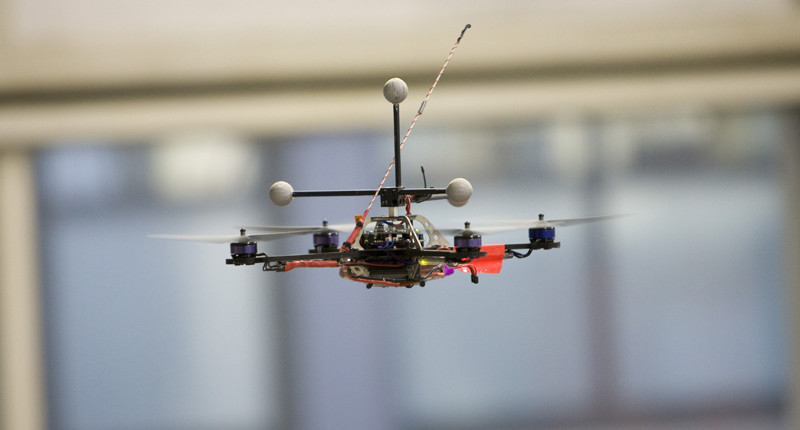
\includegraphics[width=\textwidth,height=\textheight,keepaspectratio]{flying_machine_arena.jpg}
\caption{Kvadrokopter s tremi odbojnimi označevalniki. Povzeto po \cite{fma}.}
\end{figure}

Narediti želimo podoben sistem za lokaliziranje objekta v notranjem prostoru, vendar z uporabo veliko cenejših kamer.

\section{Pregled področja}
Lokacija se večinoma določa s pomočjo triangulacije \cite{wiki:triangulation}, trilateracije \cite{wiki:trilateration} ali multilateracije \cite{wiki:multilateration}. Pri triangulaciji moramo poznati kot objekta na znano lokacijo (sidro), pri trilateraciji razdaljo od objekta do sidra, pri multilateraciji pa razliko razdalje od objekta do sidra v različnih časih. Sidra so lahko ultrazvočni in radijski oddajniki ali sprejemniki, mikrofoni, označevalniki, kamere itd. Le-ti služijo kot referenčne točke v prostoru, s katerimi se izračuna lokacija objekta.

Na Univerzi v Kaliforniji so razvili sistem, ki izračuna lokacijo s pomočjo zvoka \cite{mandal2005beep}. Za sidra so uporabili mikrofone, objekt pa je bil mobilni telefon. V $97$ \% poskusov so položaj izmerili do $50 \ cm$ natančno. Na Univerzi v Yorku so naredili podobno z Wi-Fi signali in znanim modelom zaprtega prostora \cite{chan2013dynamic}. Na Univerzi v Parani pa so za merjenje razdalje uporabili ultrazvočni signal \cite{auer20033d}. Natančnost njihovega sistema je nekaj desetink milimetra v $7\times7\times7 \ m^3$ velikem prostoru.

Zgoraj opisana dela za lokalizacijo ne uporabljajo kamer. V nadaljevanju se bomo osredotočili na dela, ki jih. Slika iz navadne kamere sama po sebi ne pove razdalje do neke točke na sliki, ampak le smer žarka, ki pa implicitno določa kot, ki ga uporabimo pri triangulaciji za določanje lokacije. Za triangulacijo potrebujemo vsaj dve sliki, ki opazujeta isti objekt iz različnih zornih kotov.

Na Univerzi v Xi’an Jiaotongu so razvili stereo sistem za določanje položaja planarne tarče \cite{li2008development}. Uporabili so dve CCD (\emph{angl. Charge-coupled Device}) \cite{wiki:ccd} kameri, ki hkrati zajameta sliko ploskve in nato iz dobjenih točk triangulirata pozicijo ploskve v prostoru. Na Tehnični univerzi v Madridu so uporabili večkamerni sistem za določanje položaja ljudi v prostoru \cite{mohedano2008robust}. Najprej segmentirajo vse premikajoče se dele slike od statičnih, saj predpostavljajo, da se bodo ljudje po prostoru premikali. Nato na teh segmentih zaznajo, kje se nahajajo ljudje. Največji problem predstavlja okluzija. Pri tem jim pomaga ravno večkamerni sistem, ki zajema slike ljudi iz različnih zornih kotov. Ko določijo, kje na slikah se nahaja glava človeka, pa lahko izračunajo njegov položaj v prostoru. Na Državni univerzi v Ohiju pa so naredili sistem \cite{lee2013real}, ki je od opisanih najbolj soroden diplomskemu delu. V prostor so postavili štiri visokoločljive omrežne kamere, ki so med seboj kalibrirane. Od štirih morata vsaj dve kameri zaznati objekt (v njihovem primeru vrtalnik), da se lahko določi njegovo lokacijo. Ko kamere prvič zaznajo objekt z ujemanjem predlog, mu pričnejo slediti. S sledenjem oz. zaznavanjem izračunajo približno sredino objekta, ki jo z večimi kamerami izpopolnijo.

\section{Cilji}
Glavni cilj diplomskega dela je ustvariti večkamerni sistem za določanje položaja objekta v prostoru. Ker se lahko zgodi, da bo pri zaznavanju prihajalo do okluzij, morata vsaj dve kameri v nekem trenutku zaznati objekt. Za obdelavo slik se bo uporabil centralni računalnik, ki bo s kamerami povezan v lokalno omrežje. Zaradi lažjega zaznavanja, bo objekt barvni označevalnik. Napaka sistema mora biti v povprečju manjša od $5 \ cm$. Določanje položaja bo delovalo v realnem času z vsaj $10$ meritvami na sekundo. Glavna omejitev sistema bo ta, da bo deloval ob predpostavki, da se v prostoru nahaja le en objekt, kar onemogoča določanje orientacije. To omejitev pa se bo lahko v prihodnosti odstranilo in bo sistem zmožen hkrati določiti položaj veliko točkam v prostoru.

\begin{figure}[H]
\centering
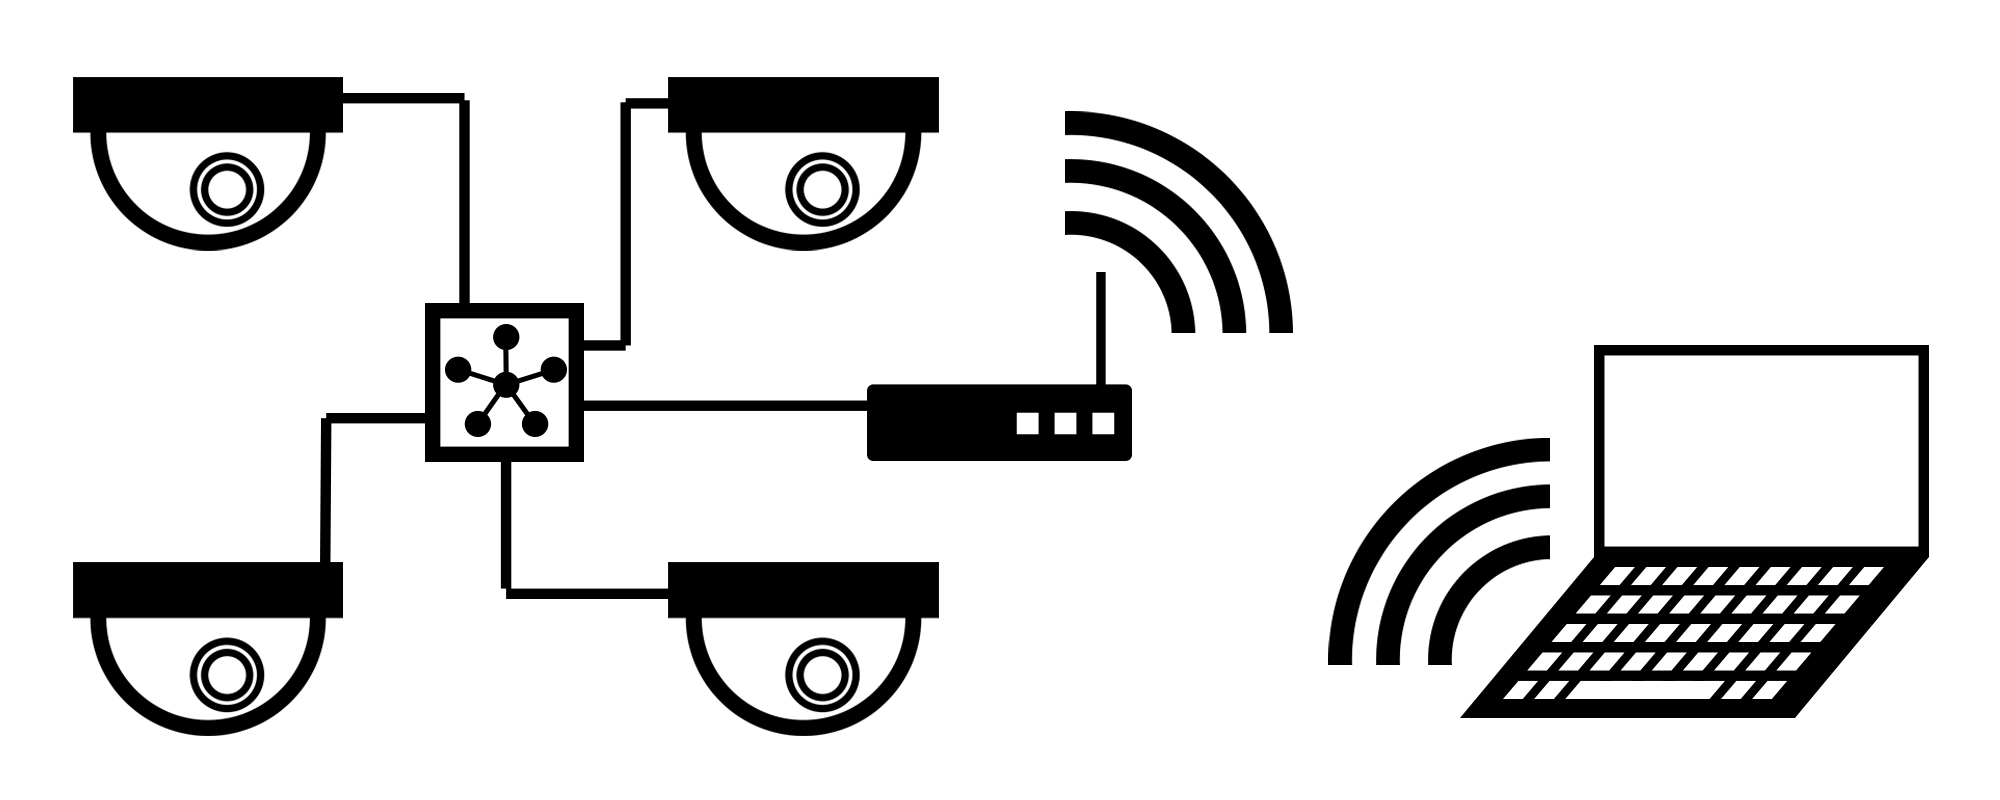
\includegraphics[height=5cm]{topology.png}
\caption{Oris večkamernega sistema.}
\label{topologyimg}
\end{figure}

\section{Struktura diplome}
Diplomsko delo je razdeljeno na pet poglavij. V uvodu je predstavljena motivacija, pregled področja in cilji dela. Drugo poglavje zajema teoretično podlago, ki je nujna za kasnejšo implementacijo rešitve. Dejansko implementacijo rešitve in konkretno uporabo prej opisane teorije opisuje tretje poglavje. V četrtem poglavju so predstavljeni rezultati dela, v zadnjem pa so poleg zaključka naslovljene tudi možne izboljšave sistema.

\chapter{Teoretična podlaga}
\section{Parametri kamere}\label{parametri}
Ugotoviti moramo, kakšen matematični model najbolj ustreza današnjim kameram. Večino kamer lahko modeliramo z modelom kamere z odprtino (\emph{angl. pinhole camera}) \cite{Hartley2004, zhang2000flexible, zhang1995robust}. Model opisuje kako se točka v svetu preslika v točko na sliki. Opišemo ga lahko s t.i. notranjimi in zunanjimi parametri kamere. V grobem, notranji parametri opisujejo interne lastnosti kamere, kot je goriščna razdalja, principalna točka, faktor poševnosti slikovnih pik itd., zunanji pa položaj kamere v prostoru.

\subsection{Notranji parametri}
Na sliki \ref{similar1} je ponazorjena preslikava točke v svetu v točko na sliki. Ugotovitve, ki smo jih pridobili v eni dimenziji lahko apliciramo tudi na drugo dimenzijo. 

\begin{figure}[H]
\centering
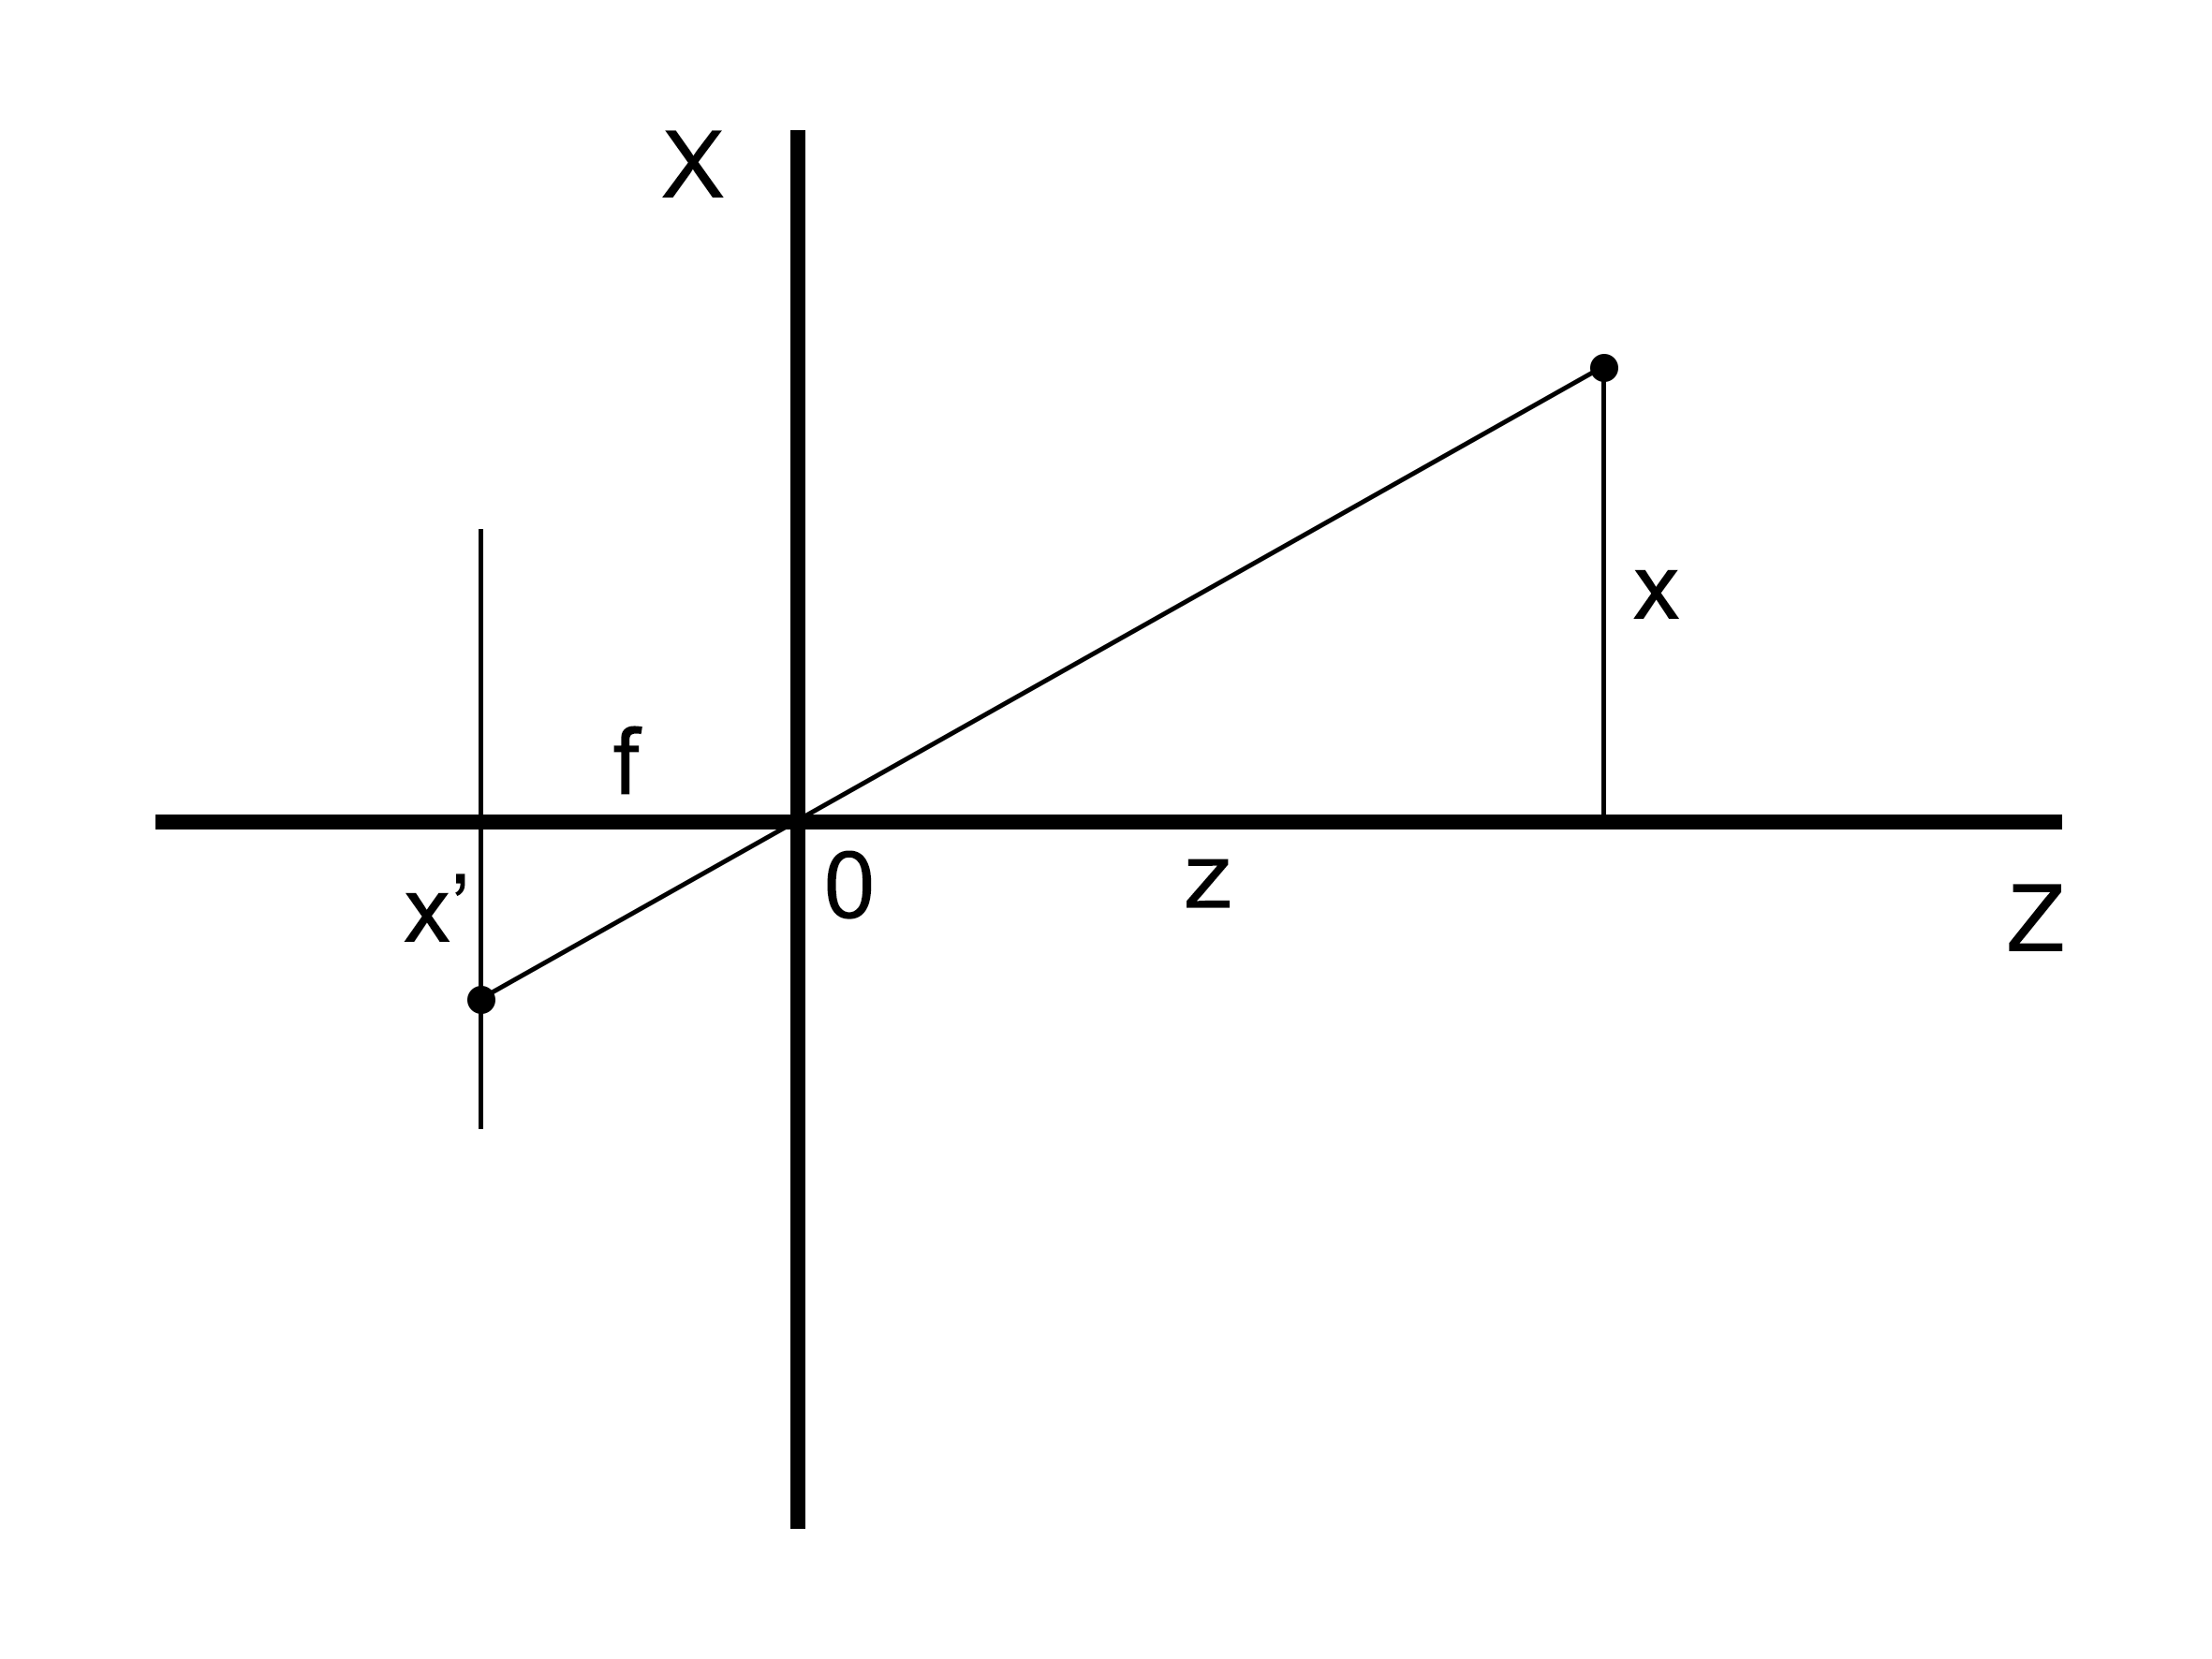
\includegraphics[width=\textwidth,height=\textheight,keepaspectratio]{similar_triangles_1.png}
\caption{Točka v svetu se preslika na slikovno ploskev $\pi$.}
\label{similar1}
\end{figure}

Koordinatno izhodišče na sliki \ref{similar1} predstavlja odprtino kamere. Višina točke v svetu je predstavljena z $x$, oddaljenost od kamere pa z $z$. Višina točke na sliki je označena z $x’$, goriščna razdalja pa s $f$. Točka v svetu se preko odprtine (koordinatnega izhodišča) prezrcali na slikovno ploskev $\pi$. Za lažje računanje pa lahko vpeljemo navidezno slikovno ploskev, kar je ponazorjeno na sliki \ref{similar2}.

\begin{figure}[H]
\centering
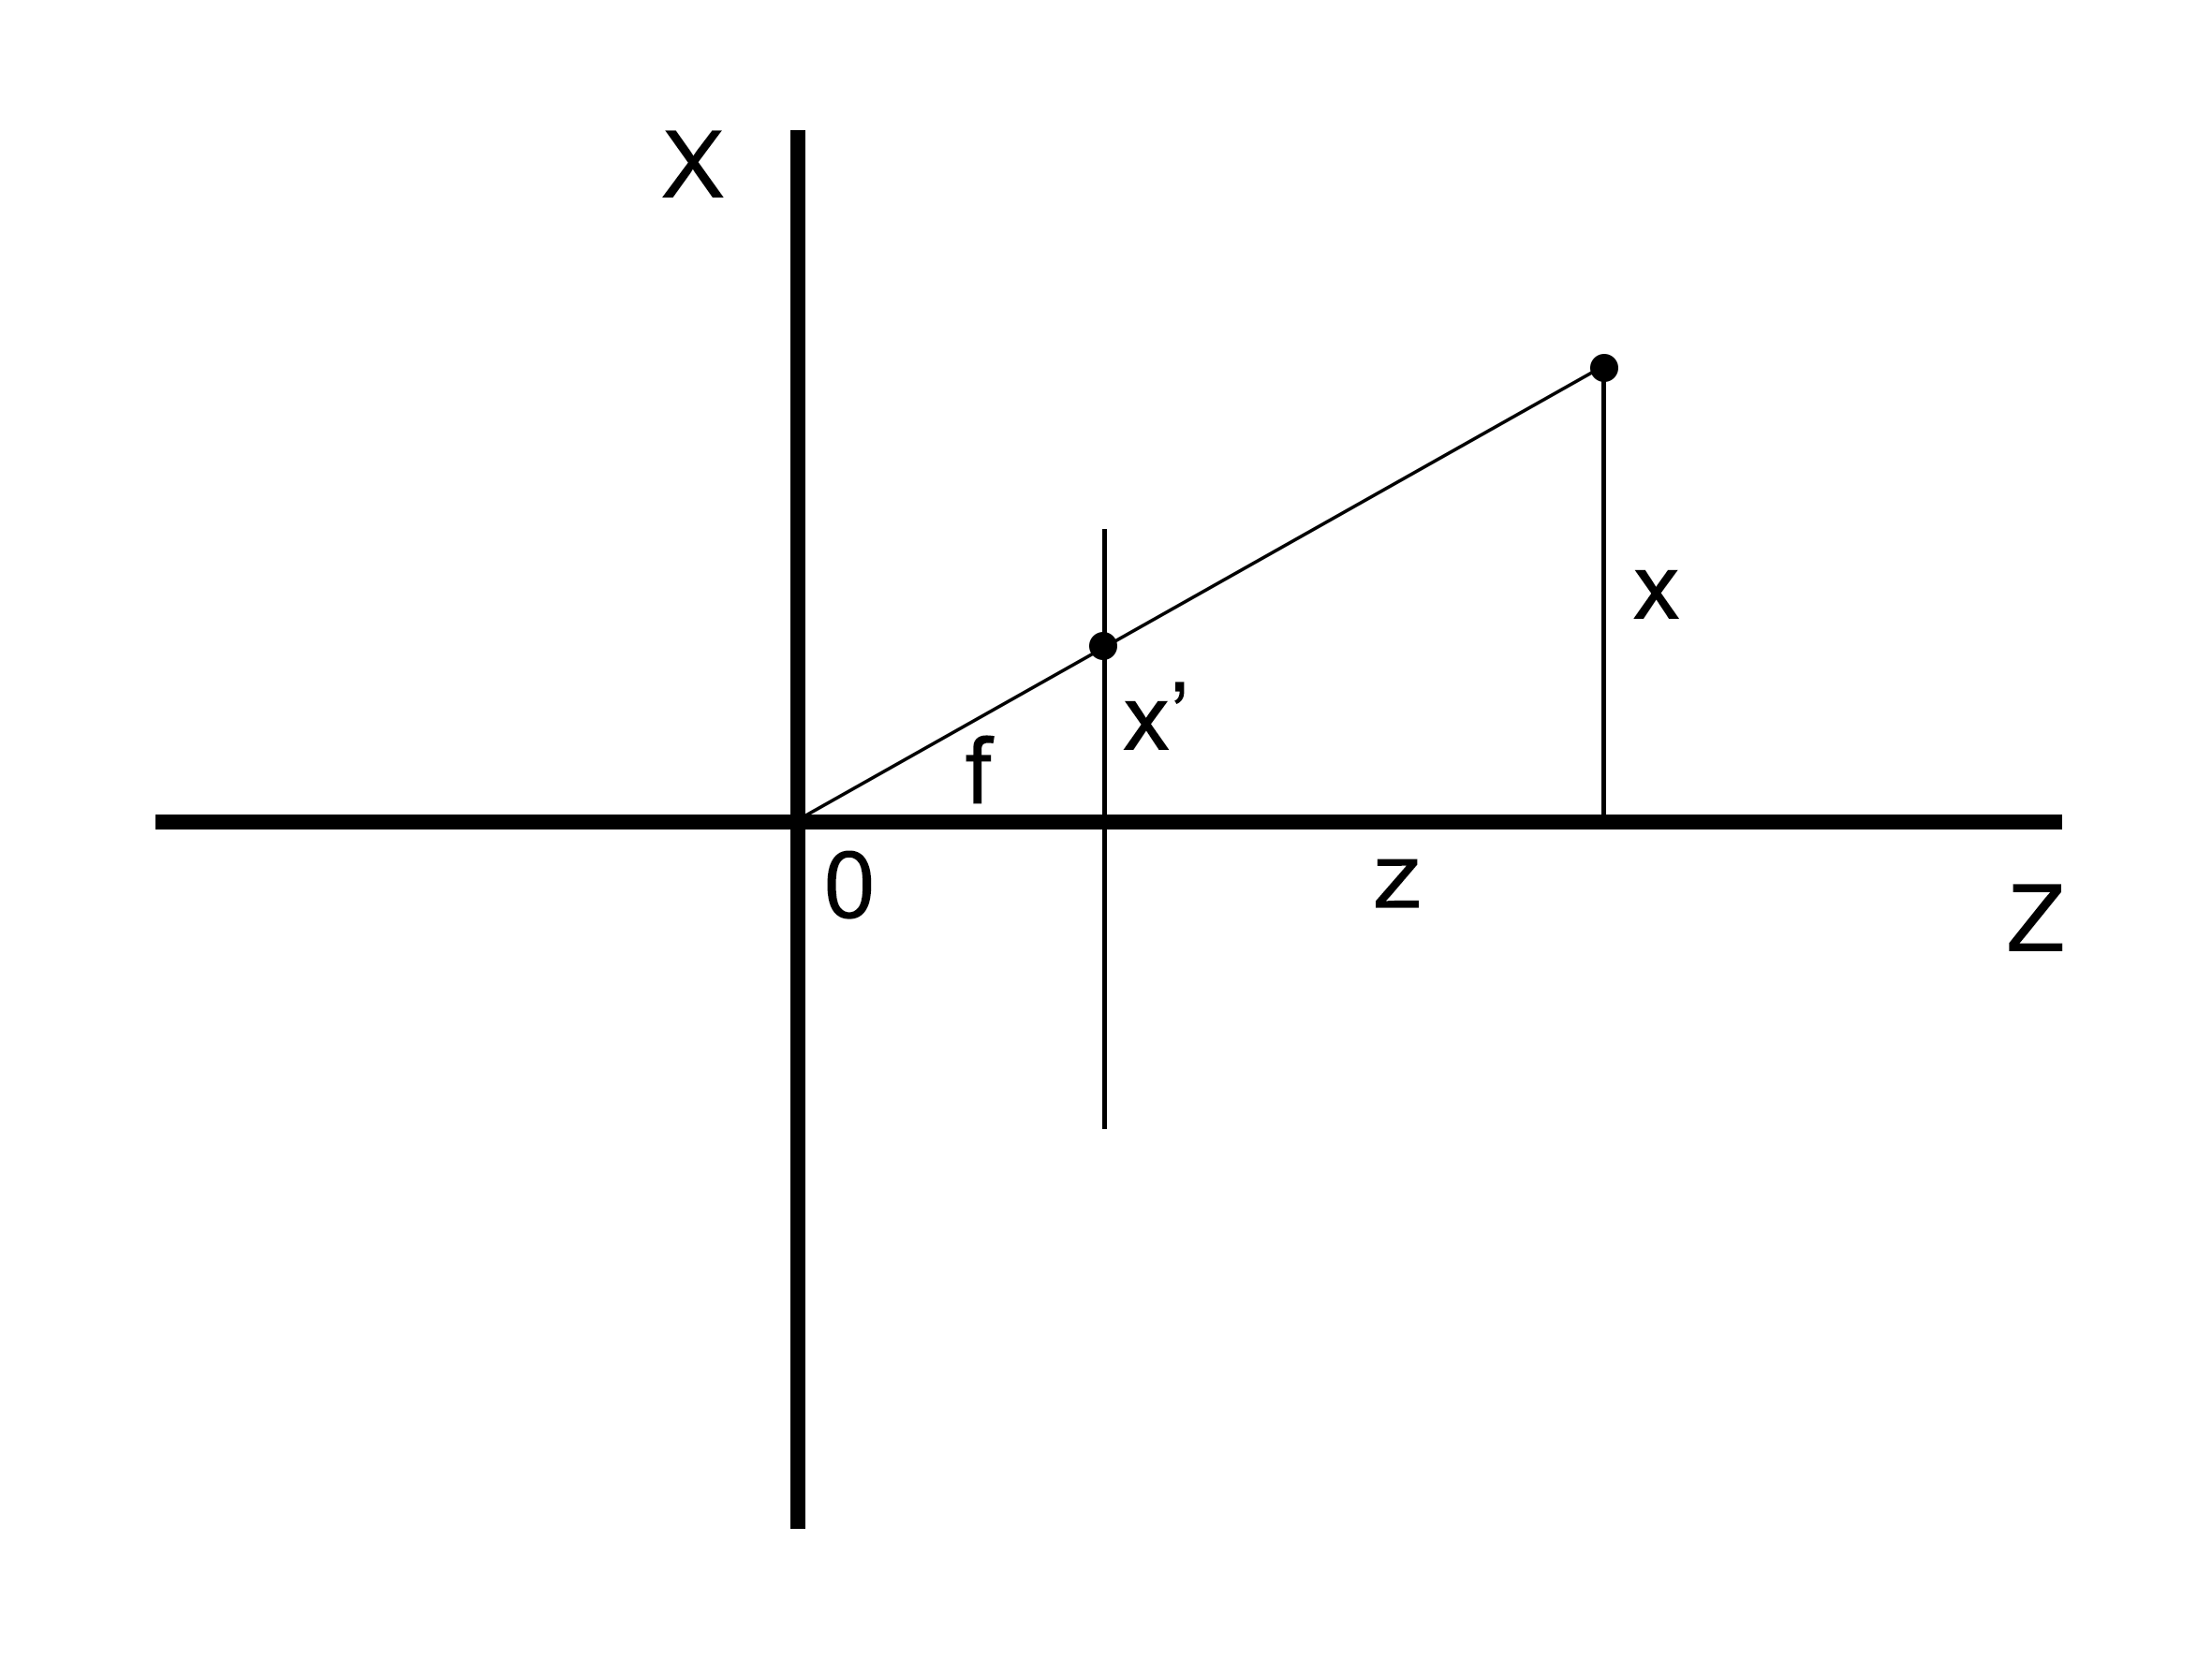
\includegraphics[width=\textwidth,height=\textheight,keepaspectratio]{similar_triangles_2.png}
\caption{Na sliki se jasno vidita dva podobna pravokotna trikotnika.}
\label{similar2}
\end{figure}

Hitro opazimo, da je preslikava iz sveta na sliko linearna operacija. Na sliki \ref{similar2} vidimo podobna pravokotna trikotnika, ki ju določa točka v svetu in točka na sliki. Vzpostavimo lahko relacijo:
\begin{align}
\frac{x'}{f} &= \frac{x}{z} \\
x' &= f \frac{x}{z}.
\end{align}
Če formulo posplošimo na obe koordinatni osi, dobimo
\begin{align}
\begin{bmatrix}
x' \\
y'
\end{bmatrix}
&= \frac{f}{z}
\begin{bmatrix}
x \\
y
\end{bmatrix}.
\label{simplemodeleq}
\end{align}

Enačba \eqref{simplemodeleq} predstavlja najpreprostejši model kamere z luknjico. Ima seveda veliko pomanjkljivosti, ki pa jih bomo postopoma odpravili. Enačbo \eqref{simplemodeleq} se da preprosteje zapisati z uvedbo homogenih koordinat.
\begin{align}
\begin{bmatrix}
x' \\
y' \\
1
\end{bmatrix}
&\sim 
\begin{bmatrix}
fx \\
fy \\
z
\end{bmatrix}
\end{align}

Točka v homogenih koordinatah ni enolično določena z vrednostmi točke, saj za homogeno točko $x$ velja $x \sim \lambda x$, kjer $\lambda \neq 0$. Homogeno točko preslikamo nazaj v evklidski prostor tako, da vse koordinate delimo z zadnjo vrednostjo točke. 

Pri predstavitvi digitalnih slik je izhodišče običajno v levem zgornjem kotu. Zgornji model pa predpostavlja izhodišče v sredini slike. V model moramo vpeljati dve konstanti $u$ in $v$, ki bosta prestavili izhodišče koordinatnega sistema slike. To se lahko kompaktno zapiše kot množenje točke v svetu z matriko \cite{Hartley2004, zhang2000flexible}.
\begin{align}
\begin{bmatrix}
x' \\
y' \\
1
\end{bmatrix}
&\sim
\begin{bmatrix}
f & 0 & u \\
0 & f & v \\
0 & 0 & 1
\end{bmatrix}
\begin{bmatrix}
x \\
y \\
z
\end{bmatrix}
\end{align}

Zgornji model predpostavlja, da so pike na senzorju kamere kvadratne. Dandanes za veliko kamer to tudi drži. Ker pa se pravokotne ali celo poševne pike lahko enostavno vključi v obstoječi model, bomo to naredili.
\begin{align}
\begin{bmatrix}
x' \\
y' \\
1
\end{bmatrix}
&\sim
\begin{bmatrix}
fm_x & s & u \\
0 & fm_y & v \\
0 & 0 & 1
\end{bmatrix}
\begin{bmatrix}
x \\
y \\
z
\end{bmatrix}
\label{internaleq}
\end{align}

Enačba \eqref{internaleq} predstavlja notranji model kamere. Goriščna razdalja je označena s $f$, $m_x$ in $m_y$ predstavljata velikost, $s$ poševnost pike, $u$ in $v$ pa določata principalno točko. Vektor $[x \ y \ z]^T$ določa točko v svetu, $[x' \ y' \ 1]^T$ pa kam se ta točka preslika na sliko.

Slike iz kamer so lahko tudi popačene. Obstajata dve vrsti popačenosti, ki ju prej opisani model ne more modelirati, in sicer radialna in tangencialna popačenost. Radialno popačenost povzroči oblika leče, poznamo pa dve glavni različici:
\begin{enumerate}
\itemsep0em
\item sodčasto, ki spominja na obliko soda in
\item blazinasto, ki spominja na obliko blazine.
\end{enumerate}
Obstaja še kombinacija obeh, ki se imenuje brkato popačenje (ker spominja na obliko brkov).

\begin{figure}[H]
\centering
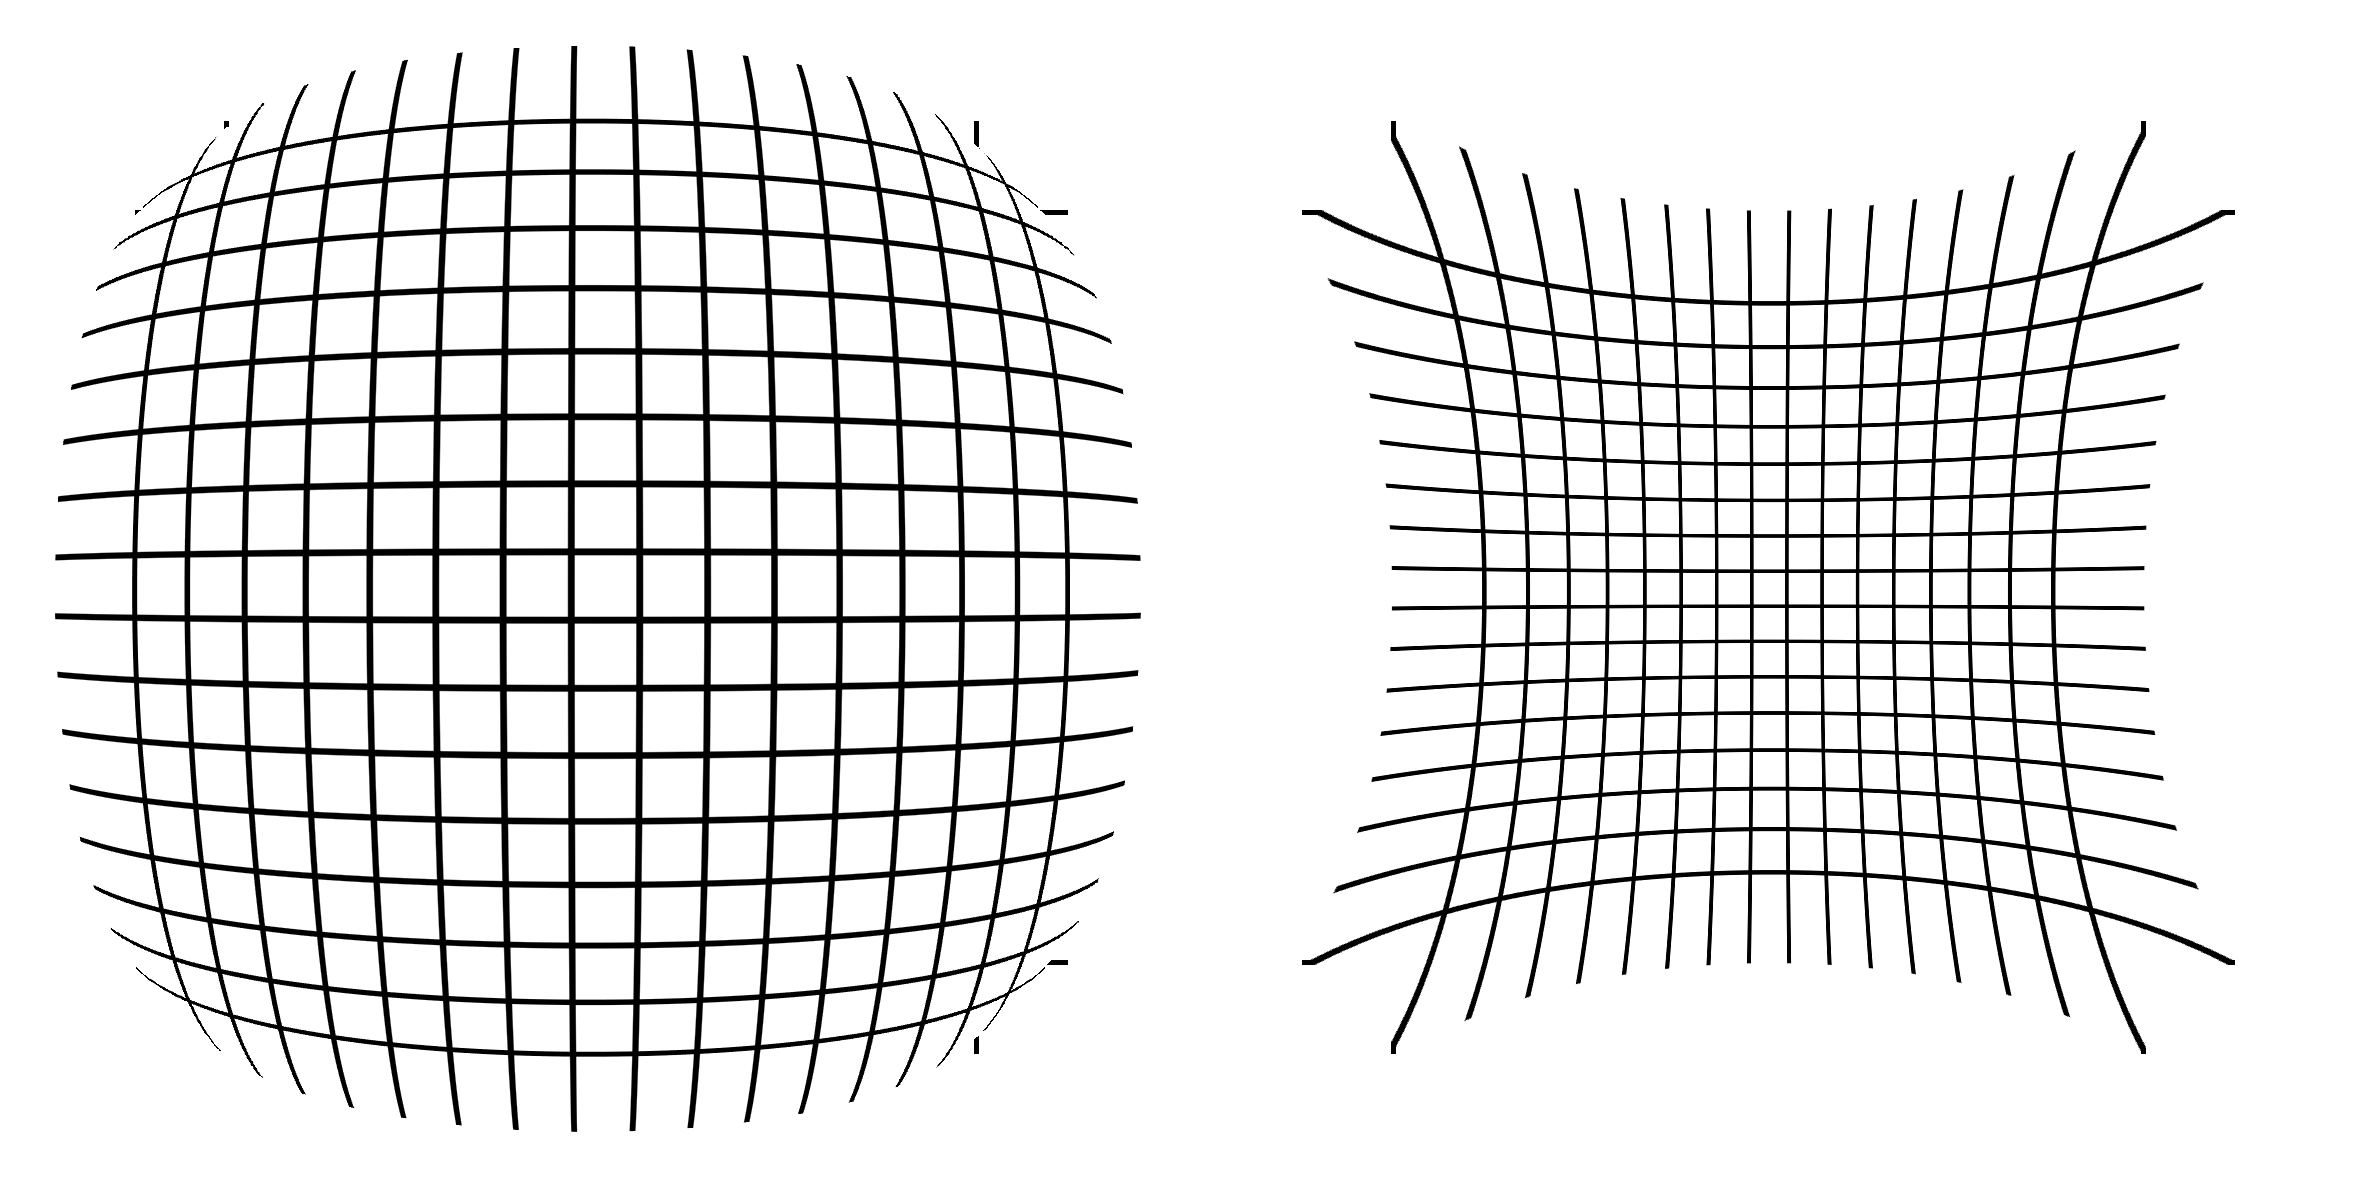
\includegraphics[width=\textwidth,height=\textheight,keepaspectratio]{distorsion.png}
\caption{Sodčasta popačenost (levo), blazinasta popačenost (desno).}
\end{figure}

Moč radialne popačenosti slikovne točke je odvisna od razdalje do principalne točke. Modeliramo jo lahko z vsotami polinomov sodih stopenj. Za večino radialnih popačenj zadoščajo trije koeficienti \cite{ Hartley2004, zhang2000flexible, brown1966decentering}. 
\begin{align}
r &= \sqrt{x^2 + y^2} \\ 
x_{popaceno} &= x(1 + k_1r^2 + k_2r^4 + k_3r^6) \\
y_{popaceno} &= y(1 + k_1r^2 + k_2r^4 + k_3r^6) \label{radialdisteq}
\end{align}

Druga popačenost, ki jo poznamo, pa je tangencialna in nastane zaradi slabe poravnanosti leč in senzorja.

\begin{figure}[H]
\centering
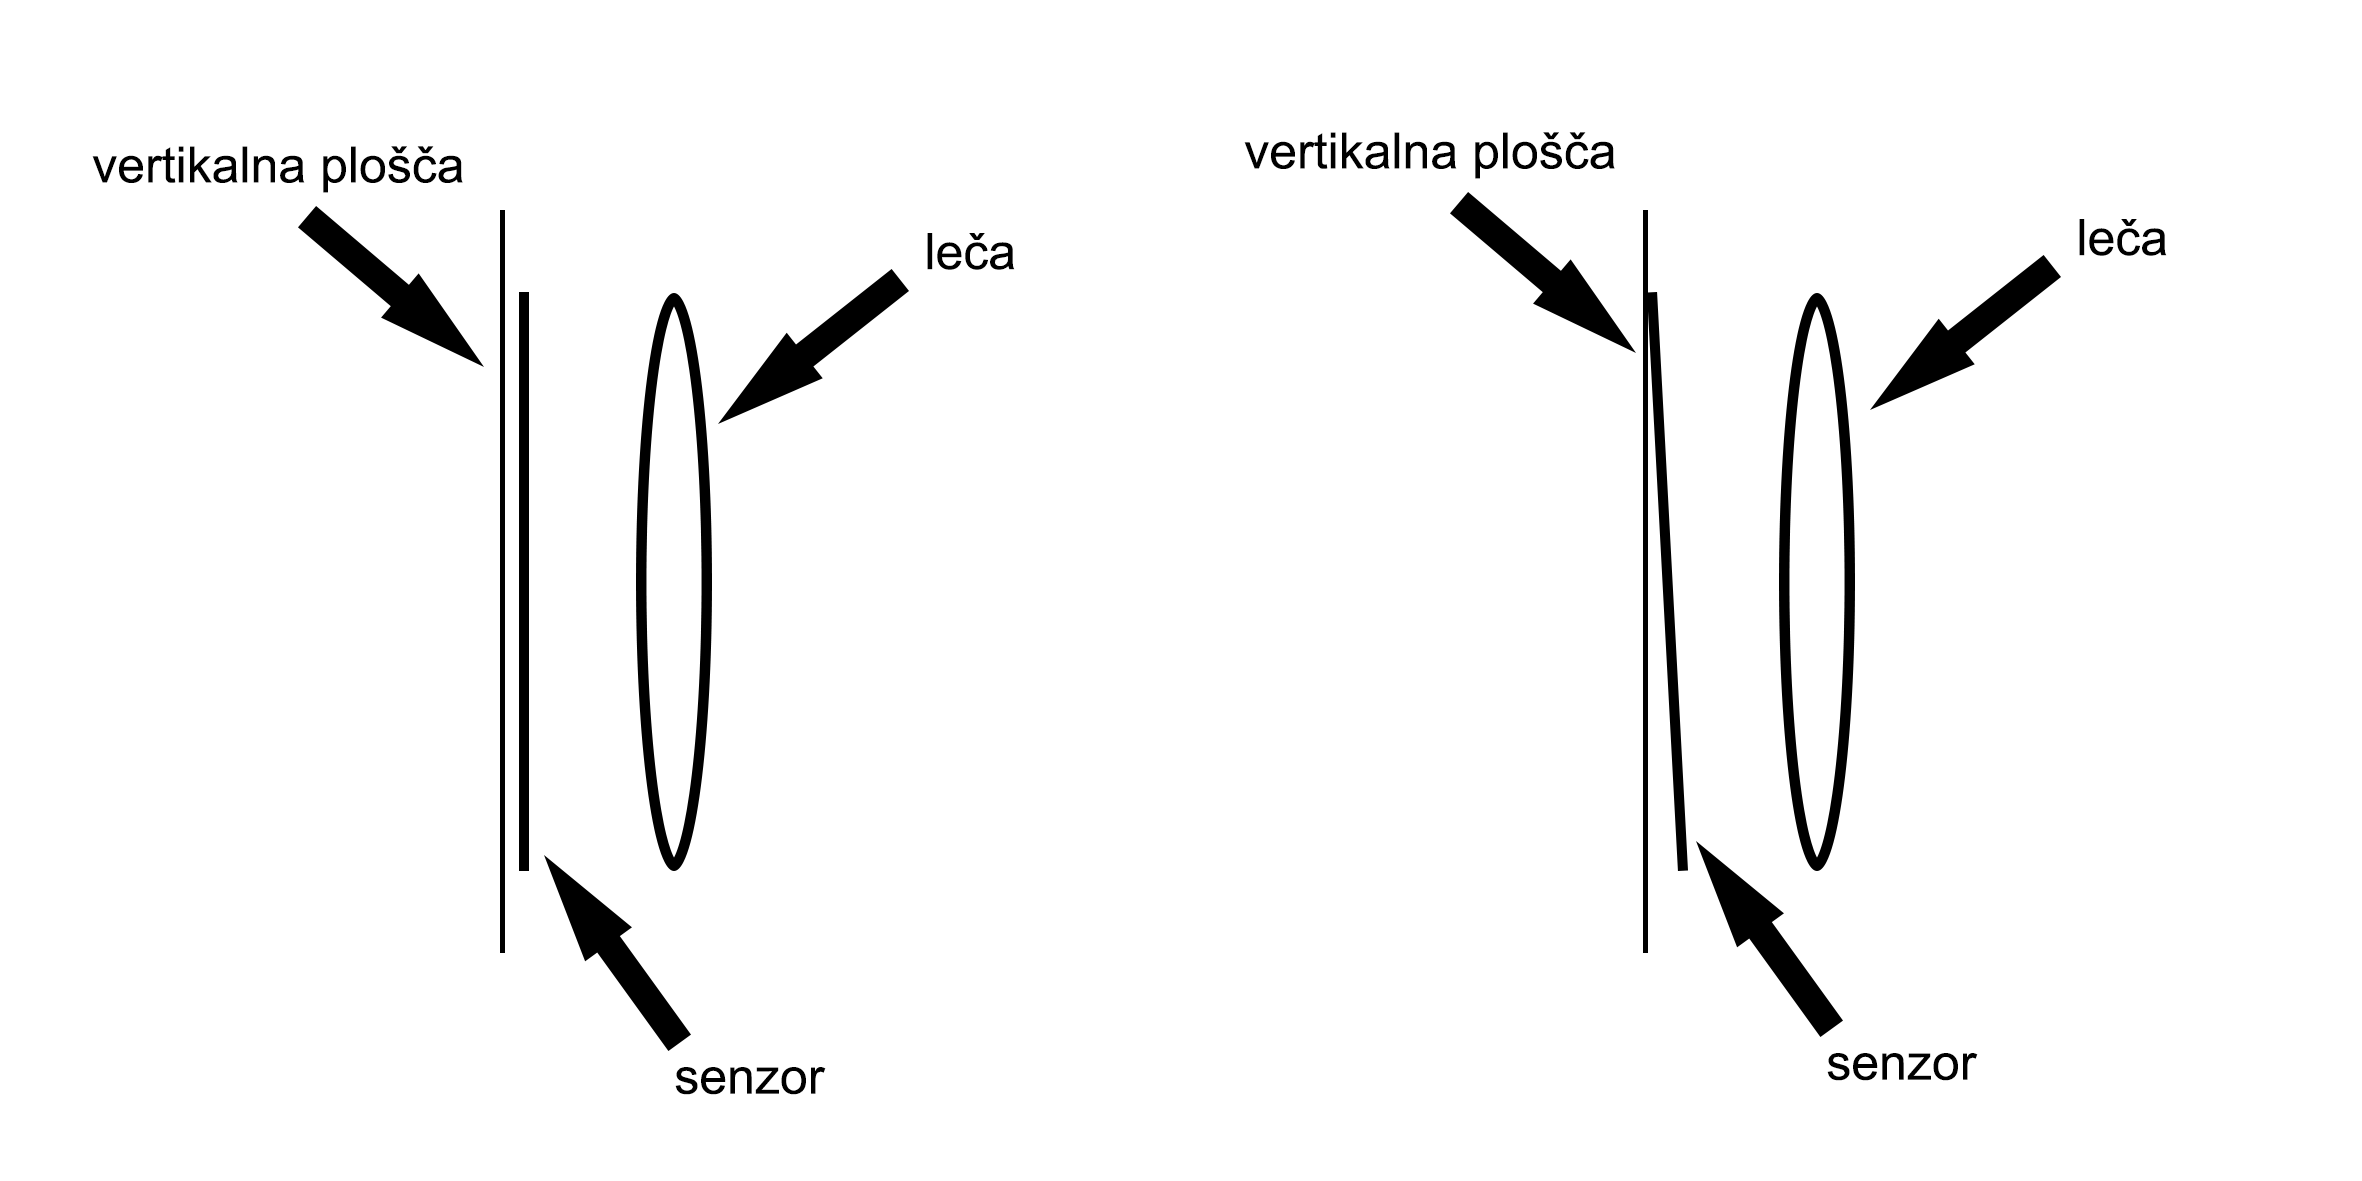
\includegraphics[width=\textwidth,height=\textheight,keepaspectratio]{tangential.png}
\caption{Leva ilustracija prikazuje kamero brez tangencialne popačenosti. Na desni ilustraciji senzor ni vzporeden leči, kar povzroči tangencialno popačenost.}
\end{figure}

Modeliramo jo lahko kot \cite{brown1966decentering}:
\begin{align}
r &= \sqrt{x^2 + y^2} \\ 
x_{popaceno} &= x + (2p_1xy + p_2(r^2 + 2x^2)) \\
y_{popaceno} &= y + (p_1(r^2 + 2y^2) + 2p_2xy). \label{tangentialdisteq}
\end{align}

Če povzamemo, notranje parametre kamere določa matrika A in koeficienti popačenja. Koeficiente se lahko predstavi z vektorjem $\vec{r}$, ki določa radialno popačenost in z vektorjem $\vec{t}$, ki določa tangencialno popačenost.
\begin{align*}
A &= 
\begin{bmatrix}
fm_x & s & u \\
0 & fm_y & v \\
0 & 0 & 1
\end{bmatrix} \\
\vec{r} &= [k_1 \ k_2 \ k_3] \\
\vec{t} &= [p_1 \ p_2]
\end{align*}

\subsection{Zunanji parametri}
Do sedaj smo predpostavljali, da je koordinatno izhodišče sveta kamera. Uporabno bi bilo, če bi lahko poljubno določili koordinatni sistem sveta in vanj postavili kamere. Ravno temu so namenjeni zunanji parametri kamere. Med različnimi koordinatnimi sistemi lahko enolično prehajamo z rotacijo in translacijo. Če napišemo malo drugače: iz enega koordinatnega sistema lahko dobimo kateri koli drug koordinatni sistem (z enakim številom dimenzij) tako, da izhodišči poravnamo s translacijo in nato rotiramo osi, da sovpadajo. 

Rotacijo v treh dimenzijah lahko predstavimo z množenjem matrike $R$, velikosti $3 \times 3$. Translacija pa je vsota točke v svetu $\vec{X}$ in translacijskega vektorja $\vec{T}$.
\begin{equation}
\vec{X}_{premaknjen} = R \vec{X} + \vec{T} = 
\begin{bmatrix}
r_{11} & r_{12} & r_{13} \\
r_{21} & r_{22} & r_{23} \\
r_{31} & r_{32} & r_{33}
\end{bmatrix}
\begin{bmatrix}
x \\
y \\
z 
\end{bmatrix}
+
\begin{bmatrix}
x_t \\
y_t \\
z_t 
\end{bmatrix}
\label{coordeq}
\end{equation}

Izkaže se, da če točko v svetu predstavimo s homogenimi koordinatami, lahko enačbo \eqref{coordeq} zapišemo kot množenje matrike $[R | \vec{T}]$ z vektorjem $\vec{X}$.
\begin{equation}
\vec{X}_{premaknjen} = [R|\vec{T}] \vec{X} = 
\begin{bmatrix}
r_{11} & r_{12} & r_{13} & x_t\\
r_{21} & r_{22} & r_{23} & y_t\\
r_{31} & r_{32} & r_{33} & z_t
\end{bmatrix}
\begin{bmatrix}
x \\
y \\
z \\
1
\end{bmatrix}
\label{coordeq}
\end{equation}
Zavedati se moramo, da rotacijska matrika $R$ in translacijski vektor $\vec{T}$ ne predstavljata rotacije in pozicije kamere v svetu, ampak rotacijo in pozicijo sveta relativno na kamero. Rotacijo kamere lahko dobimo z $R^{-1} = R^T$, pozicijo v svetu pa z $-R^{-1} \vec{T} = -R^T \vec{T}$.

\subsection{Model kamere}

Model \eqref{internaleq} lahko dopolnimo z zunanjimi parametri in tako dobimo popoln model kamere.
\begin{align}
\label{totalmodel}
\vec{X}' &\sim A[R | \vec{T}] \vec{X} \\
\begin{bmatrix}
x' \\
y' \\
1
\end{bmatrix}
&\sim
\begin{bmatrix}
fm_x & s & u \\
0 & fm_y & v \\
0 & 0 & 1
\end{bmatrix}
\begin{bmatrix}
r_{11} & r_{12} & r_{13} & x_t\\
r_{21} & r_{22} & r_{23} & y_t\\
r_{31} & r_{32} & r_{33} & z_t
\end{bmatrix}
\begin{bmatrix}
x \\
y \\
z \\
1
\end{bmatrix} \\
\vec{r} &= [k_1 \ k_2 \ k_3 \dots] \\
\vec{t} &= [p_1 \ p_2]
\end{align}

\section{Ocenjevanje parametrov}
V poglavju \ref{parametri} je opisan model kamere. Kamero določajo razni parametri, ki pa so za vsako kamero različni. V tem poglavju bomo opisali, kako oceniti posamezne parametre kamere, da bo model postal uporaben.

\subsection{Ocenjevanje notranjih parametrov}
Za ocenjevanje notranjih parametrov kamere obstaja veliko algoritmov, ki se razlikujejo po hitrosti, težavnosti in natančnosti. Dve popularni metodi sta Tsaijev kalibracijski algoritem \cite{horn2000tsai} in Zhangova fleksibilna tehnika za kalibracijo kamer \cite{zhang2000flexible}. V nalogi smo za kalibracijo notranjih parametrov uporabil MATLAB-ov kalibrator kamere \cite{matlabcalib}, ki uporablja variacijo Zhangove tehnike. Več o samem postopku kalibracije je opisano v poglavju \ref{camcalsec}. 

\subsection{Ocenjevanje zunanjih parametrov}\label{externalparamssection}
Zunanji parametri kamere določajo kje v prostoru se kamera nahaja. Zgoraj omenjena Zhangova metoda poleg notranjih vrne tudi zunanje parametre, ki pa za namen diplomskega dela niso uporabni, saj bi morali kamere kalibrirati z vsaj eno sliko ploskve, ki jo v celoti vidijo vse kamere in bi morala biti dovolj velika. Sistem mora delovati tudi, če imajo nekatere kamere med seboj minimalno ali celo prazno prekrivanje vidnega polja. V nadaljevanju bomo opisali teoretično podlago metode, ki smo jo uporabili za ocenjevanje zunanjih parametrov. Doseči želimo, da kameram določimo skupni koordinatni sistem sveta.

Metoda predpostavlja, da imamo za neko kamero že izračunane notranje parametre. Za oceno zunanjih parametrov je dovolj le ena slika iz kamere, ki pa ne sme biti popačena, zato moramo popačeno sliko najprej popraviti. Enačbi \eqref{radialdisteq} in \eqref{tangentialdisteq} določata neposredno preslikavo med popačenimi in nepopačenimi točkami. 

Zunanje parametre določa rotacijska matrika $R$ in translacijski vektor $\vec{T}$, kar je v enačbi \eqref{cammodeleq} kompaktno predstavljeno z matriko $[R | \vec{T}]$. Za oceno teh parametrov moramo poznati notranje parametre $A$, točko v svetu $X$ in njeno projekcijo na sliko $X'$. Matriko $[R | \vec{T}]$ lahko ocenimo z metodo DLT (\emph{angl. Direct Linear Transformation}) \cite{Hartley2004}. Ker računamo s homogenimi koordinatami, sta si leva in desna stran enačbe enaki do poljubnega neničelnega faktorja $\lambda$.
\begin{align}
\vec{X}' &\sim A[R | \vec{T}] \vec{X} \label{cammodeleq} \\
\lambda \vec{X}' &= A[R | \vec{T}] \vec{X} \label{lambdaeq}
\end{align}

Z eno znano točko (na sliki in v svetu) dobimo tri enačbe, vendar pa je ena linearna kombinacija drugih dveh, zato nam pri ocenjevanju zunanjih parametrov ne pomaga. Oceniti moramo torej $12$ neznank (ker je matrika $[R | \vec{T}]$ velika $3 \times 4$) z eno točko pa dobimo dve neodvisni enačbi, kar pomeni, da potrebujemo najmanj šest točk, za katere poznamo svetovne koordinate in njihove projekcije na sliko. Dobimo torej sistem enačb,

\begin{align*}
\lambda_1 \vec{X}_1' &= A[R | \vec{T}] \vec{X_1} \\
\lambda_2 \vec{X}_2' &= A[R | \vec{T}] \vec{X_2} \\
\lambda_3 \vec{X}_3' &= A[R | \vec{T}] \vec{X_3} \\
&\vdots
\end{align*}

Problem predstavljajo neničelni faktorji na levi strani enačb, saj jih ne poznamo in so odvisni od zunanjih parametrov kamere. Metoda DLT reši ravno tak sistem enačb. Leva stran je pravzaprav 3-dimenzionalni vektor za katerega vemo, da je vedno enak nič, če ga vektorsko pomnožimo s samim seboj. Vektorsko množenje pa lahko predstavimo z matričnim množenjem.
\begin{align}
\vec{a} &= 
\begin{bmatrix}
a_1 \\
a_2 \\
a_3
\end{bmatrix} \\
\vec{a} \times \vec{a} = [\vec{a}]_{\times} \vec{a} &= 
\begin{bmatrix}
0 & -a_3 & a_2 \\
a_3 & 0 & -a_1 \\
-a_2 & a_1 & 0
\end{bmatrix}
\begin{bmatrix}
a_1 \\
a_2 \\
a_3
\end{bmatrix} = 0
\end{align}

Obe strani enačbe \eqref{lambdaeq} lahko pomnožimo z leve z $[\vec{X}']_{\times}$.
\begin{align}
\lambda [\vec{X}']_{\times} \vec{X}' &= [\vec{X}']_{\times} A[R | \vec{T}] \vec{X} \\
0 &= [\vec{X}']_{\times} A[R | \vec{T}] \vec{X}
\end{align}

S tem korakom smo se znebili neznanega parametra $\lambda$, vendar iz take oblike enačbe težko najdemo rešitev sistema. Za lažjo izpeljavo bomo enačbo \eqref{lambdaeq} z leve pomnožili z inverzom matrike $A$.

\begin{align}
\label{uvw}
A^{-1} \vec{X}' &=
\begin{bmatrix}
u \\
v \\
w
\end{bmatrix} \\
[A^{-1} \vec{X}']_{\times} &=
\begin{bmatrix}
0 & -w & v \\
w & 0 & -u \\
-v & u & 0
\end{bmatrix} \\[5ex]
\lambda A^{-1} \vec{X}' &= [R | \vec{T}] \vec{X} \\
0 &= [A^{-1} \vec{X}']_{\times} [R | \vec{T}] \vec{X}\\
0 &= 
\begin{bmatrix}
0 & -w & v \\
w & 0 & -u \\
-v & u & 0
\end{bmatrix}
\begin{bmatrix}
p_1 & p_2 & p_3 & p_4 \\
p_5 & p_6 & p_7 & p_8 \\
p_9 & p_{10} & p_{11} & p_{12}
\end{bmatrix}
\begin{bmatrix}
x \\
y \\
z \\
1
\end{bmatrix} \\
0 &= 
\begin{bmatrix}
x(-wp_5 + vp_9) + y(-wp_6 + vp_{10}) + z(-wp_7 + vp_{11}) + (-wp_8 + vp_{12}) \\
x(wp_1 - up_9) + y(wp_2 - up_{10}) + z(wp_3 - up_{11}) + (wp_4 - up_{12}) \\
x(-vp_1 + up_5) + y(-vp_2 + up_6) + z(-vp_3 + up_7) + (-vp_4 + up_8)
\end{bmatrix}
\label{longeq}
\end{align}

\setcounter{MaxMatrixCols}{20}
Sistem enačb \eqref{longeq} lahko zapišemo v obliki $B \vec{p} = 0$, kjer
\begin{align}
\vec{p} &= [p_1 \ p_2 \ p_3 \ p_4 \ p_5 \ p_6 \ p_7 \ p_8 \ p_9 \ p_{10} \ p_{11} \ p_{12}]^T \\
B &=
\begin{bmatrix}
0 & 0 & 0 & 0 & -xw & -yw & -zw & -w & xv & yv & zv & v \\
xw & yw & zw & w & 0 & 0 & 0 & 0 & -xu & -yu & -zu & -u \\
-xv & -yv & -zv & -v & xu & yu & zu & u & 0 & 0 & 0 & 0
\end{bmatrix}.
\label{bmatrix}
\end{align}

Zadnja vrstica v matriki $B$ je linearna kombinacija prvih dveh. Za vsak par točk (v svetu in na sliki) generiramo prvi dve vrstici matrike $B$ in vse vrstice združimo v skupno matriko $B$ velikosti $2n \times 12$, kjer je $n$ število parov točk. Sistem enačb lahko sedaj rešimo z razcepom na singularne vrednosti (\emph{angl. SVD - Singular Value Decomposition}). SVD razcepi matriko $B$ na $U \Sigma V^T$, kjer je $U$ matrika levih lastnih vektorjev, $\Sigma$ matrika singularnih vrednosti in $V$ matrika desnih lastnih vektorjev. Po definiciji za leve lastne vektorje matrike $B$ velja $B \vec{v} = \lambda \vec{v}$, kjer je $\lambda$ lastna vrednost. Če iz matrike $V$ vzamemo vektor, ki ustreza najmanjši lastni vrednosti v matriki $\Sigma$, smo tako dobili netrivialno rešitev, ki najbolje zadošča pogoju $B \vec{p} = 0$. Rešitev je potrebno le še preoblikovati v $3 \times 4$ matriko zunanjih parametrov. V poglavju \ref{camcalsec} naslovimo problem, ki nastane, če matrika $B$ nima ranga $12$, kar se zgodi, če ocenjujemo parametre s koplanarnimi točkami v prostoru.

\section{Triangulacija}

Iz modela \eqref{totalmodel} želimo oceniti $\vec{X}$. Uporabimo lahko podoben postopek kot pri ocenjevanju zunanjih parametrov.

\begin{align}
\lambda \vec{X}' &= A[R | \vec{T}] \vec{X} \\
0 &= [\vec{X}']_{\times} A[R | \vec{T}] \vec{X} \\
B &= [\vec{X}']_{\times} A[R | \vec{T}] \\
B \vec{X} &= 0
\end{align}

Rang matrike $B$ mora biti štiri, saj ocenjujemo štiri parametre, ki določajo $X$. Ena točka na sliki nam poda dve linearno neodvisni enačbi. Potrebujemo torej vsaj dve različni točki iz dveh različnih slik, ki predstavljata projekcijo iste točke v prostoru na sliko. Sistem zopet rešimo z razcepom na singularne vrednosti, kot smo to naredili v prejšnjem poglavju.

\chapter{Implementacija}

\section{Strojna oprema}

\subsection{Računalnik}
Vsa obdelava podatkov se odvija na enem prenosnem računalniku, zajemanje slik pa poteka sočasno v ločenih procesih. Računalnik, ki ima dve fizični procesni jedri in štiri niti, je v lokalno omrežje je povezan preko brezžične povezave. 

\begin{table}[H]
\centering
\begin{tabular}{| r | l |}
\hline
CPE & Intel i7-4510U 2.6 GHz \\
Pomnilnik & 8 GB \\
Št. jeder/niti & 2 / 4 \\
Arhitektura & 64-bit \\
OS & Windows 8.1 Pro \\
\hline
\end{tabular}
\caption{Specifikacije računalnika.}
\end{table}

\subsection{Kamere}
V nalogi uporabljamo štiri Axis 215 PTZ omrežne kamere. To so varnostne IP kamere, primarno namenjene nadzoru okolja. Kamere so povezane v zvezdišče na omrežju ethernet, zvezdišče pa je povezano z brezžičnim usmerjevalnikom (slika \ref{topologyimg}).  Kamere so zmožne v realnem času preko lokalnega omrežja posredovati do 30 slik na sekundo pri ločljivosti $704 \times 576$. Vseeno pa varnostne kamere niso namenjene sinhroniziranemu zajemanju slik in ne podpirajo skupnega prožilca. Največja ločljivost je $704 \times 576$, kar je relativno malo za pozicioniranje objekta v $7,5 \times 7,5 \times 3 \ m^3$ velikem prostoru.
\begin{figure}[H]
\centering
\includegraphics[width=\textwidth,height=\textheight,keepaspectratio]{axis_215_ptz.png}
\caption{Axis 215 PTZ kamera.}
\end{figure}

\begin{table}[H]
\centering
\begin{tabular}{| r | l |}
\hline
Tip kamere & varnostna IP \\
Hitrost zajemanja & 30 FPS \\
Formati pretoka & MPEG-4, MJPEG \\
Največja ločljivost & 704 $\times$ 576 \\
Optična povečava & 12$\times$ \\
Digitalna povečava & 4$\times$ \\
Povezava z omrežjem & ethernet \\
Leča & 3,8 - 46 mm \\
\hline
\end{tabular}
\caption{Specifikacije Axis 215 PTZ.}
\end{table}

Axis kamere imajo CGI (\emph{angl. Common Gateway Interface}) vmesnik, ki omogoča nadzor funkcionalnosti preko protokola HTTP (\emph{angl. Hypertext Transfer Protocol}). Vsak model kamere podpira različen nabor ukazov, katerih spisek lahko dobimo z GET zahtevkom na naslov:
\begin{center}
\texttt{http://<ip-kamere>/axis-cgi/com/ptz.cgi?info=1}
\end{center}
Vsi ukazi so podani kot parameter v zahtevku:
\begin{center}
\texttt{http://<ip-kamere>/axis-cgi/com/ptz.cgi?<ukaz>=<vrednost>} .
\end{center}
Spodaj je prikazan izpis ukaza \texttt{info=1} na Axis 215 PTZ kameri.
\begin{lstlisting}
Available commands
:
{camera=[n]}
whoami=yes
center=[x],[y]
   imagewidth=[n]
   imageheight=[n]
move={ home | up | down | left | right | upleft | upright | downleft | downright | stop }
pan=[abspos]
tilt=[abspos]
zoom=[n]
focus=[n]
rpan=[offset]
rtilt=[offset]
rzoom=[offset]
rfocus=[offset]
brightness=[offset]
rbrightness=[offset]
autofocus={ on | off }
ircutfilter={ on | off | auto }
backlight={ on | off }
continuouspantiltmove=[x-speed],[y-speed]
continuouszoommove=[speed]
continuousfocusmove=[speed]
auxiliary=[function]
setserverpresetname=[name]
setserverpresetno=[n]
removeserverpresetname=[name]
gotoserverpresetname=[name]
gotoserverpresetno=[n]
barcoord=[x],[y]
   panbar=[length],{ horizontal | vertical }
   tiltbar=[length],{ horizontal | vertical }
   zoombar=[length],{ horizontal | vertical }
   focusbar=[length],{ horizontal | vertical }
   irisbar=[length],{ horizontal | vertical }
   brightnessbar=[length],{ horizontal | vertical }
speed=[n]
query={ speed | position | presetposcam | presetposall }
\end{lstlisting}

%\vspace{2ex}

\section{Programska oprema}
Delo smo začeli v programskem okolju MATLAB R2014a. MATLAB je visokonivojski programski jezik in razvojno okolje, ki je primarno namenjeno prototipiranju. Podpira računanje z visokonivojskimi strukturami kot so matrike in vektorji. V MATLAB-u smo razvili konceptno rešitev, ki jo kasneje implementiramo v Python aplikaciji. 

Za zajemanje statičnih slik iz kamer smo uporabili Node.js v0.12.3. Node.js je JavaScript pogon z veliko različnimi moduli. Njegova arhitektura je po zasnovi asinhrona, kar pri vhodno/izhodnih operacijah močno pohitri sistem.

Za iskanje kamer v omrežju smo uporabili Axisov IPUtility, ki samodejno vrne IP naslove vseh kamer, ki so priključene v omrežje.

Za implementacijo glavnega sistema smo uporabili Python 2.7 s knjižnicami Numpy v1.9.2, SciPy v0.15.1 ter OpenCV v3.0.0. Morda se zdi Python za realnočasovni sistem slaba izbira, vendar je s pravilno uporabo knjižnic odlično orodje za hitri razvoj aplikacij. Funkcije v knjižnicah so zaradi hitrosti implementirane v nižjenivojskih jezikih kot sta C in C++. Knjižnica Numpy je namenjena računanju z matrikami, SciPy pa je njena razširitev. OpenCV (Open Computer Vision) pa je namenjen za probleme umetnega zaznavanja in pri svoji implementaciji uporablja strukture Numpy-ja. 

\section{Kalibracija kamer}\label{camcalsec}
\subsection{Ocenjevanje notranjih parametrov}
Za ocenjevanje notranjih parametrov uporabimo MATLAB-ov kalibrator kamere. Za kalibracijo mu moramo podati slike šahovnice, ki so bile zajete s kamero, ki jo želimo kalibrirati. Širina šahovnice mora biti različna od višine, da lahko enolično določimo njeno orientacijo. 
\begin{figure}[H]
\centering
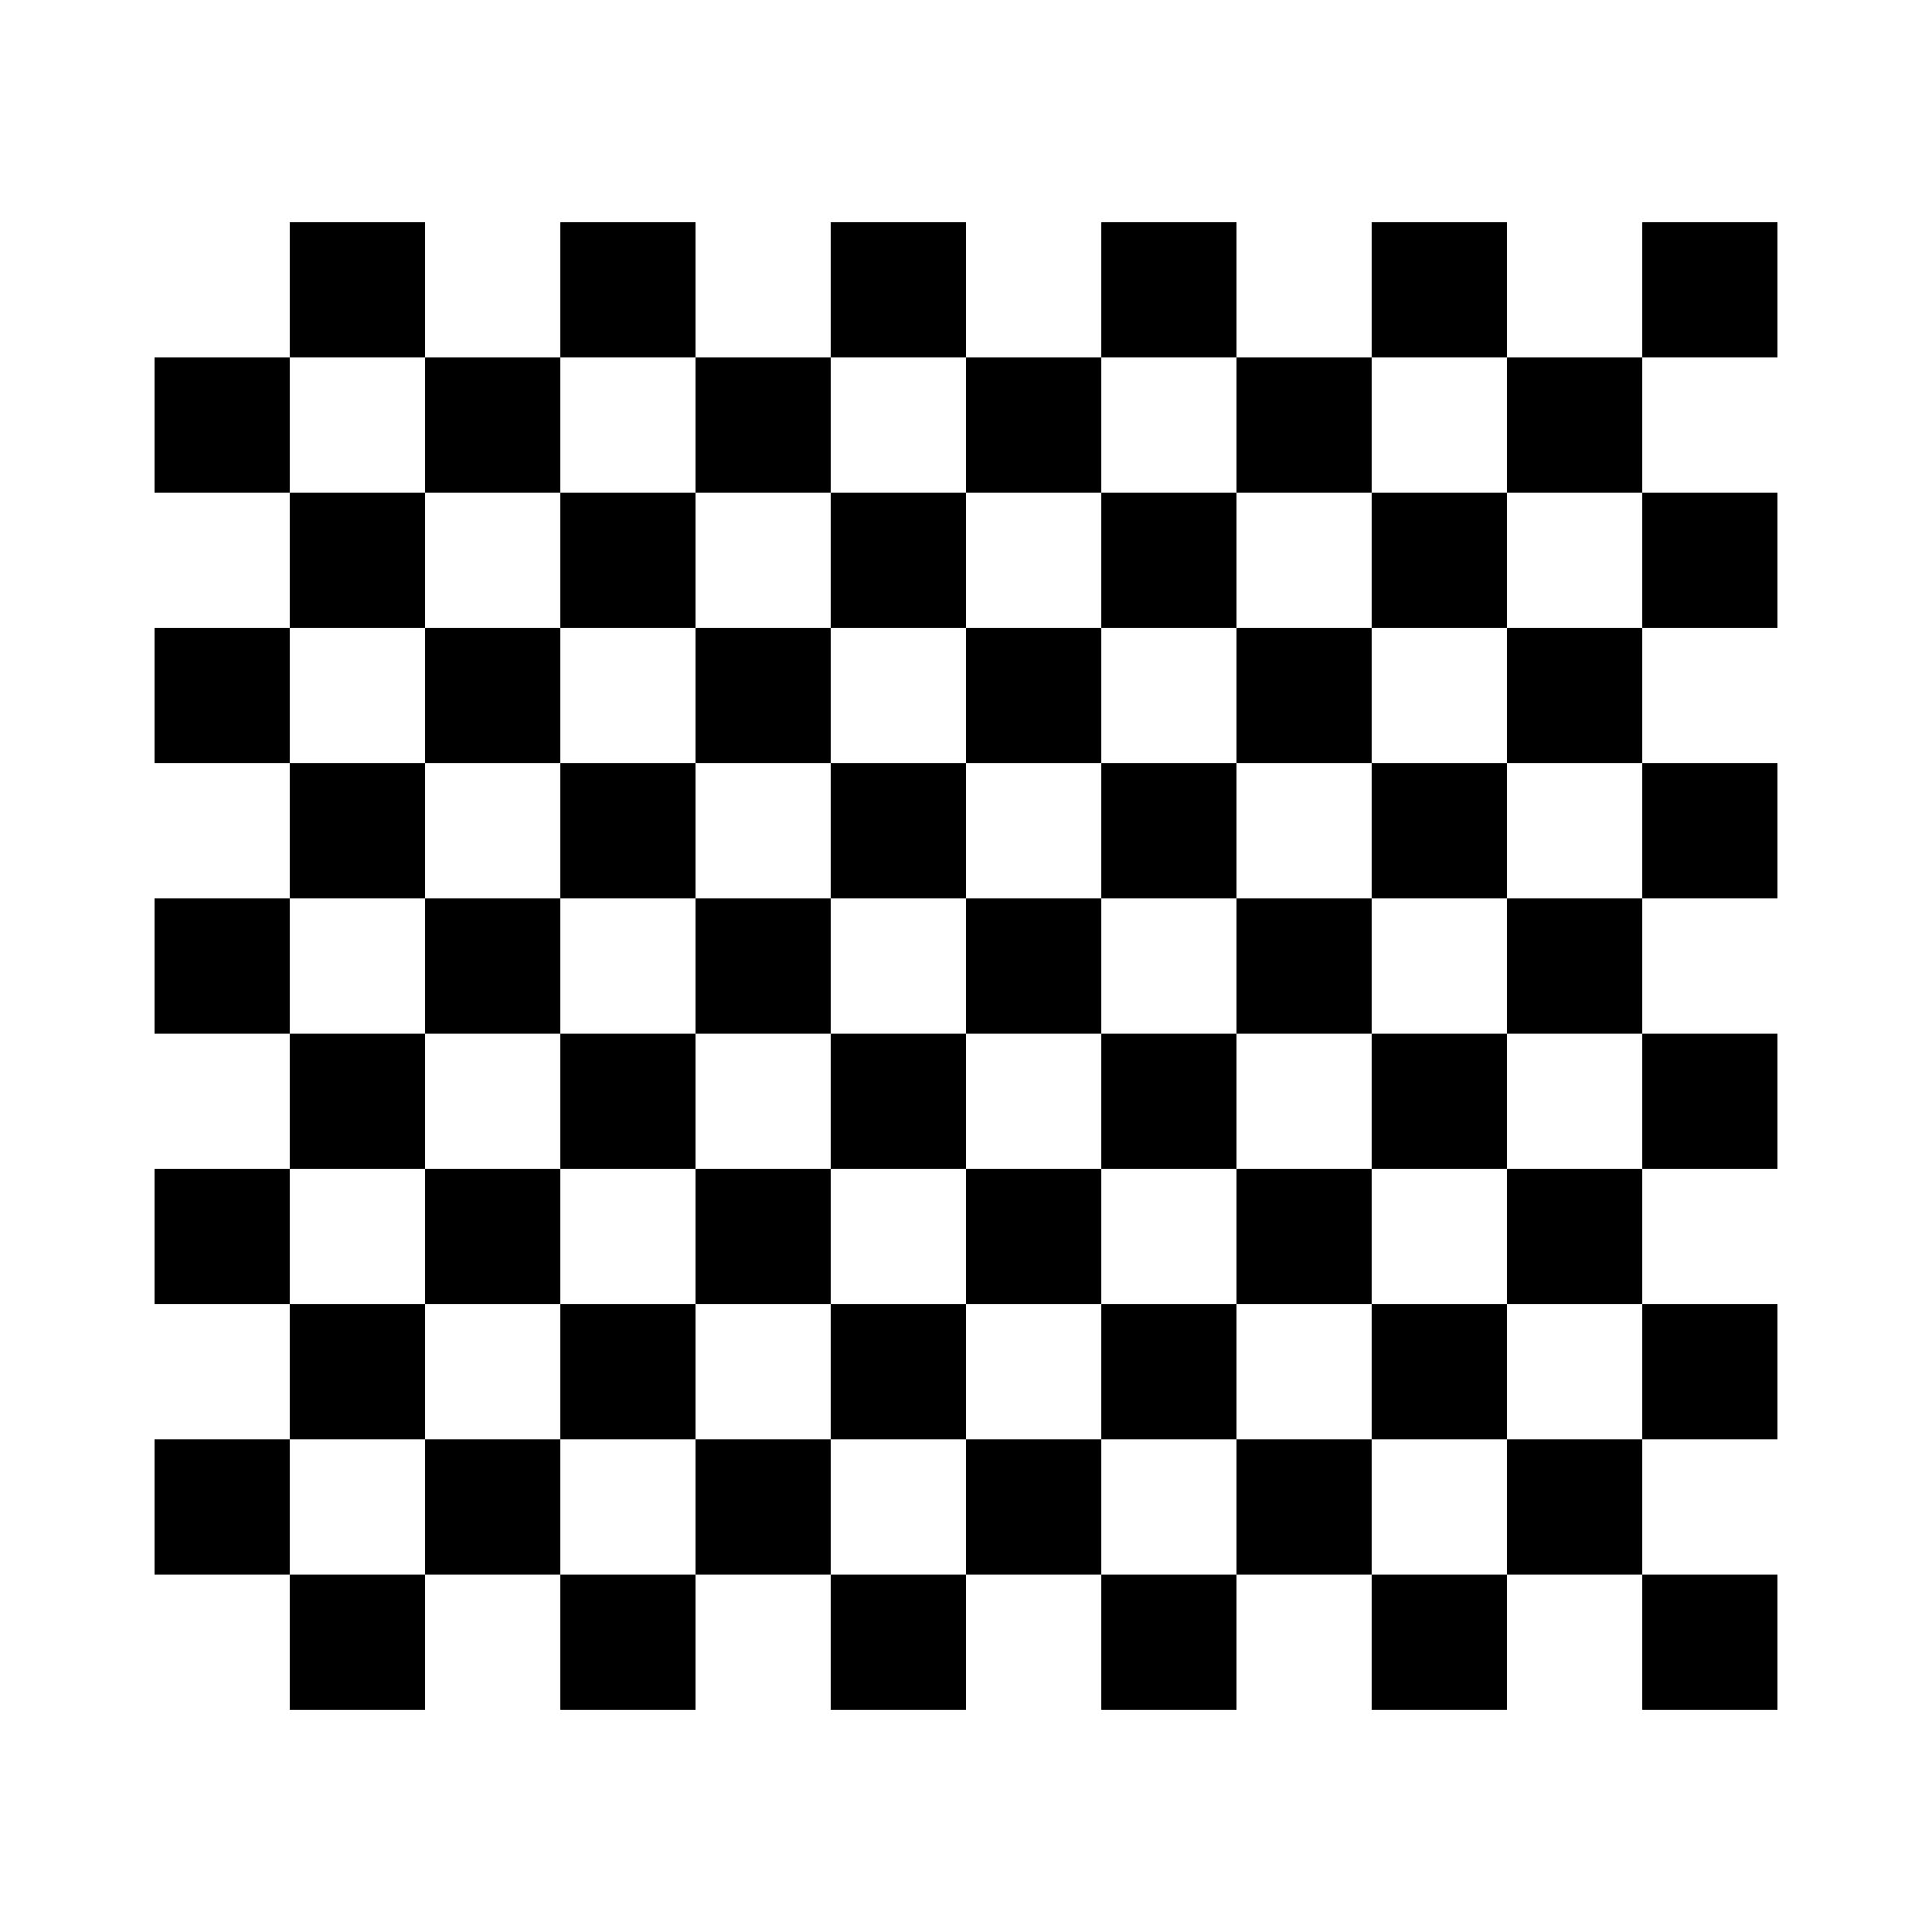
\includegraphics[scale=0.4]{checkerboard.png}
\caption{Šahovnica velikosti 11 $\times$ 12.}
\end{figure}

Za učinkovito kalibracijo notranjih parametrov moramo zajeti okoli 10 - 20 slik z različnimi orientacijami in translacijami šahovnice. Postopek kalibracije z orodjem je sledeč:
\begin{enumerate}
\itemsep0em
\item zajamemo slike šahovnice;
\item naložimo jih v orodje za kalibracijo;
\item izberemo število koeficientov za radialno popačenost (privzeto dva);
\item obkljukamo ali želimo oceniti poševnost in tangencialno popačenost;
\item kalibriramo;
\item postopek lahko ponavljamo s podmnožico slik na podlagi reprojekcijske napake, in
\item ocenjene notranje parametre izvozimo za uporabo.

\end{enumerate}
\begin{figure}[H]
\centering
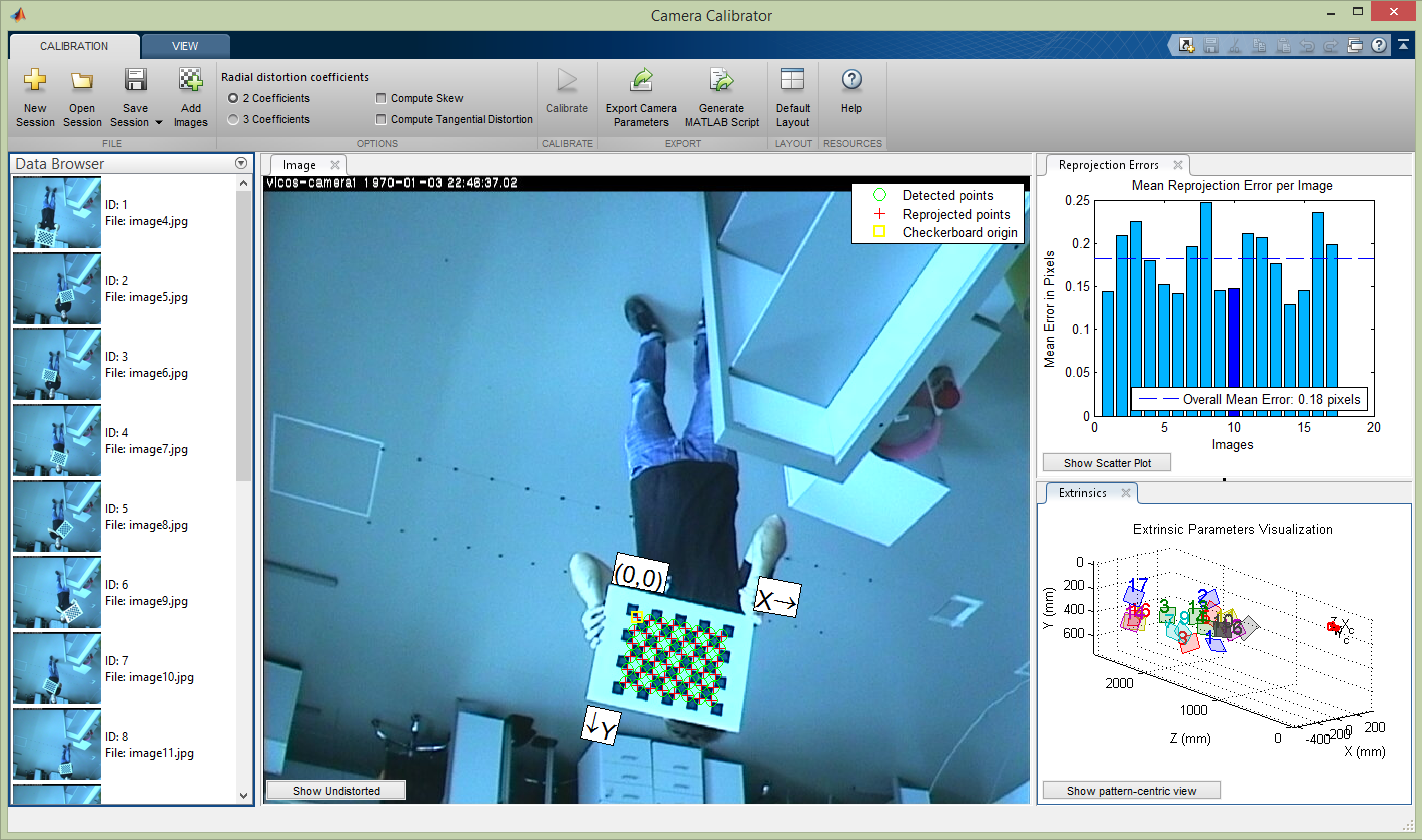
\includegraphics[width=\textwidth,height=\textheight,keepaspectratio]{internal_calibration.png}
\caption{Na sliki se vidi zaznane robove šahovnice in njena orientacija, graf reprojekcijske napake (razlaga v \ref{reprojectioncalibsection}) in vizualizacija zunanjih parametrov.}
\end{figure}

\begin{figure}[H]
\centering
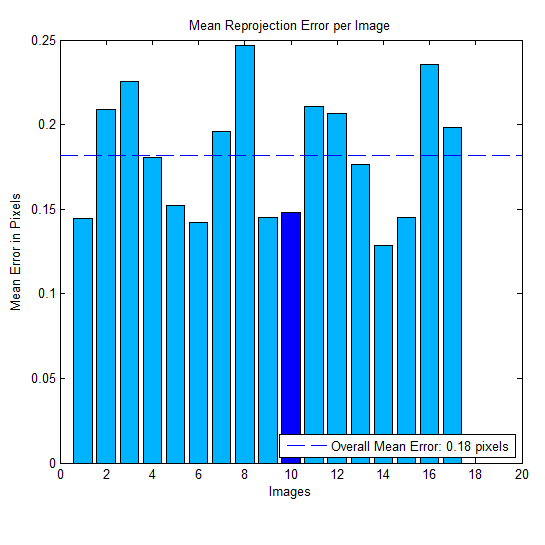
\includegraphics[scale=0.35]{reprojection_error.png}
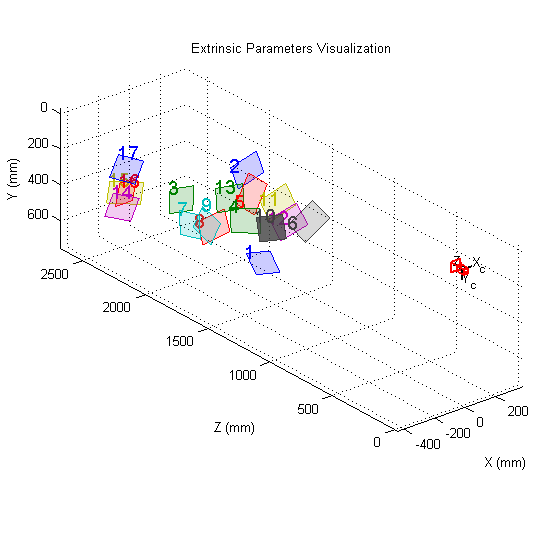
\includegraphics[scale=0.35]{extrinsic_visualization.png}
\caption{Graf reprojekcijske napake za vsako sliko (levo) in vizualizacija pozicij šahovnic s središčem v kameri (desno). }
\end{figure}

\begin{figure}[H]
\begin{align}
A &= 
\begin{bmatrix}
761,6027 & 0 & 386,6599 \\
0 & 835,939 & 362,0371 \\
0 & 0 & 1
\end{bmatrix} \\
\vec{r} &= [-0,2934 \ 0,1331] \\
\vec{t} &= [0.0006 \ 0,0012]
\end{align}
\caption{Primer ocenjenih notranjih parametrov ene izmed kamer. Tangencialna popačenost je skoraj zanemarljiva.}
\end{figure}


\subsection{Ocenjevanje zunanjih parametrov}
Ocenjevanje zunanjih parametrov je pravzaprav postavljanje kamere v nek skupni koordinatni sistem sveta. Določiti moramo rotacijsko matriko $R$ in translacijski vektor $\vec{T}$, ki predstavljata kje se nahaja koordinatni sistem relativno na kamero. Za oceno parametrov uporabimo metodo, ki je opisana v poglavju \ref{externalparamssection}. Potrebujemo le eno sliko, na kateri lahko določimo točke v svetu. V prostoru smo določili in označili koordinatni sistem. Med oznakami na osi $x$ je razdalja $20 \ cm$, na osi $y$ pa $60 \ cm$. Enota je $1 \ cm$.

\begin{figure}[H]
\centering
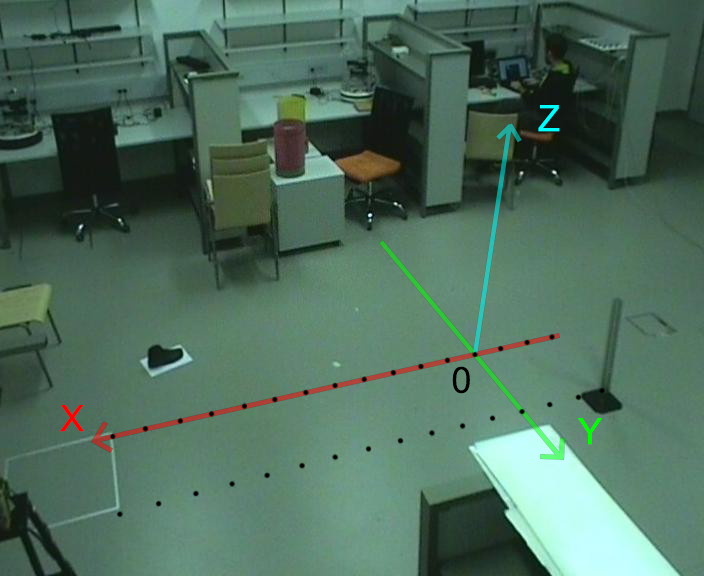
\includegraphics[width=\textwidth,height=\textheight,keepaspectratio]{coord_system.png}
\caption{Na sliki se vidi označen koordinatni sistem sveta. Točke označene s črnimi pikami so koplanarne in z njimi določimo zunanje parametre kamere.}
\label{coordsystemimg}
\end{figure}

Najprej moramo določiti pare $(\vec{X}, \vec{X'})$, ki določajo preslikavo med točko v svetu in točko na sliki. Imeti moramo minimalno šest parov, ker moramo oceniti $12$ parametrov (devet za rotacijsko matriko in tri za translacijo), en par pa nam določi dve linearno neodvisni enačbi. Točke v svetu določimo sami, nato pa jih ročno ali avtomatsko označimo na sliki. Če je slika kakorkoli popačena, jo moramo popraviti.

\begin{table}[H]
\centering
\begin{tabular}{| c | c | c | c | c |}
\hline
x & y & z & x' & y' \\
\hline
240 & 0 & 0 & 591.1441 & 139.8898 \\
200 & 0 & 0 & 523.8898 & 156.1610 \\
160 & 0 & 0 & 460.9746 & 171.3475 \\
120 & 0 & 0 & 399.1441 & 185.4492 \\
80 & 0 & 0 & 340.5678 & 198.4661 \\
40 & 0 & 0 & 284.1610 & 211.4831 \\
0 & 0 & 0 & 229.9237 & 223.4153 \\
-40 & 0 & 0 & 177.8559 & 234.2627 \\
240 & 60 & 0 & 584.6356 & 62.8729 \\
200 & 60 & 0 & 508.7034 & 83.4831 \\
160 & 60 & 0 & 437.1102 & 101.9237 \\
120 & 60 & 0 & 368.7712 & 119.2797 \\
80 & 60 & 0 & 303.6864 & 135.5508 \\
40 & 60 & 0 & 241.8559 & 150.7373 \\
0 & 60 & 0 & 183.2797 & 165.9237 \\
-40 & 60 & 0 & 125.7881 & 177.8559 \\
\hline
\end{tabular}
\caption{16 parov točk dobljenih iz slike \ref{coordsystemimg}.}
\label{pointpairs}
\end{table}

V tabeli \ref{pointpairs} se lepo vidi, da so vse točke v svetu koplanarne, saj je pri vseh $z = 0$. Sedaj lahko določimo matriko $B$, ki je za en par točk definirana v enačbi \eqref{bmatrix}. Za vsak par točk dodamo nove vrstice matriki $B$ in tako dobimo matriko velikosti $2n \times 12$ oz. $3n \times 12$ (če izračunamo tudi zadnjo vrstico, ki je redundantna), kjer je $n$ število parov točk. Zavedati se moramo, da so $u, v, w$ določeni z enačbo \eqref{uvw}, kjer uporabimo matriko notranjih parametrov $A$. S tem korakom odstranimo matriko $A$ iz matrike $A [R|\vec{T}]$ in s tem lažje določimo matriko $[R|\vec{T}]$. Z razcepom na singularne vrednosti rešimo sistem $B \vec{p} = 0$ in dobljeno rešitev preoblikujemo v $3 \times 4$ matriko zunanjih parametrov. Rešitev je pravzaprav deveti stolpec matrike $V$, ki jo vrne SVD in ne dvanajsti, kot je opisano pri izpeljavi teorije. To je posledica koplanarnosti svetovnih točk. Matrika $B$ je ranga 9, ker je komponenta $z$ vseh točk v svetu enaka 0. Spodnja matrika prikazuje primer rešitve za pare točk iz tabele \ref{pointpairs}.
\begin{equation}
[R|\vec{T}] = 
\begin{bmatrix}
-0.0018 & 0.0006 & 0 & 0.1989 \\
0.0003 & 0.0007 & 0 & 0.1607 \\
0.0005 & 0.0016  & 0 & -0.9668 \\
\end{bmatrix}
\end{equation}

Hitro opazimo, da podmatrika $R$ ni prav nič podobna rotacijski matriki. Stolpci rotacijskih matrik so paroma ortonormirani. Ker računamo s homogenimi koordinatami, lahko dobljeno matriko pomnožimo z neničelnim skalarjem, brez da bi pri tem uničili model kamere. Sedaj lahko ročno popravimo podmatriko $R$, da bo karseda podobna rotacijski matriki.
\begin{align}
[R|\vec{T}] = [\vec{R_1} \ \vec{R_2} \ \vec{R_3} \ \vec{T}] &\sim \frac{1}{||R_1||}
\begin{bmatrix}
-0.0018 & 0.0006 & 0 & 0.1989 \\
0.0003 & 0.0007 & 0 & 0.1607 \\
0.0005 & 0.0016  & 0 & -0.9668 \\
\end{bmatrix} \\
[R|\vec{T}] &\sim
\begin{bmatrix}
-0.9544 & 0.3003 & 0 & 106.6226 \\
0.1419 & 0.3877 & 0 & 86.1440 \\
0.2627 & 0.8810 & 0 & -518.2979 \\
\end{bmatrix}
\end{align}

Sedaj sta prva dva stolpca ortonormirana oz. skoraj ortonormirana (odvisno od natančnosti ocene parametrov). Čas je, da naslovimo še zadnji problem rotacijske matrike. Zaradi prej omenjene koplanarnosti je tretji stolpec ničelni vektor. Vemo, da mora biti ta paroma ortonormiran s prvima stolpcema, zato ga lahko določimo z vektorskim produktom.

\begin{align}
R_3 &= R_1 \times R_2 =
\begin{bmatrix}
-0.9544 \\
0.1419 \\
0.2627
\end{bmatrix}
\times
\begin{bmatrix}
0.3003 \\
0.3877 \\
0.8810
\end{bmatrix} \\
R_3 &= 
\begin{bmatrix}
0.0232 \\
0.9197 \\
-0.4127
\end{bmatrix}
\end{align}

Zdaj moramo le še določiti pravo smer novo izračunanega vektorja. $R_3$ kot tudi $-R_3$ sta legalni rešitvi in implicitno določata sučnost koordinatnega sistema. Pravilno rešitev določimo ročno na podlagi projekcije točk, kot je vidno iz slike \ref{reprojectionwrongimg}.

\begin{figure}[H]
\centering
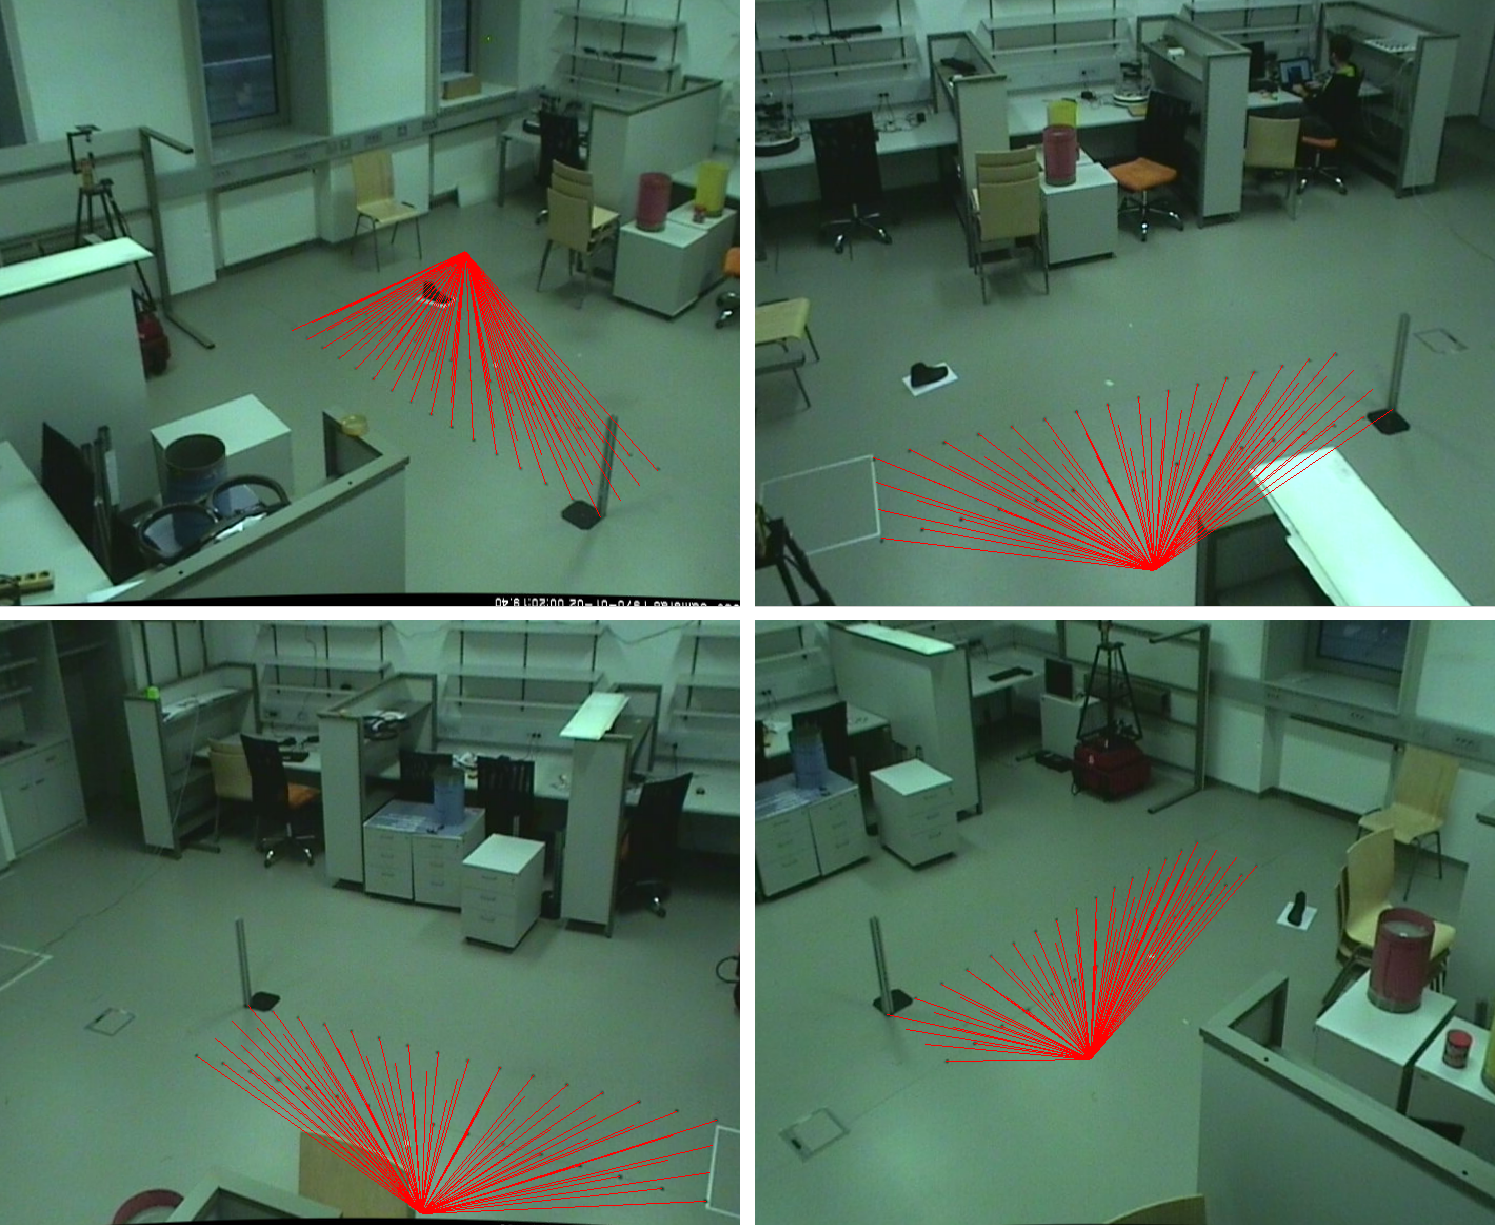
\includegraphics[scale=0.25]{reprojection_wrong.png}
\caption{Projekcija piramide na sliko pokaže, da so zadnji trije koordinatni sistemi levosučni, zato moramo obrniti smer zadnjega stolpca matrike $R$.}
\label{reprojectionwrongimg}
\end{figure}

\begin{figure}[H]
\centering
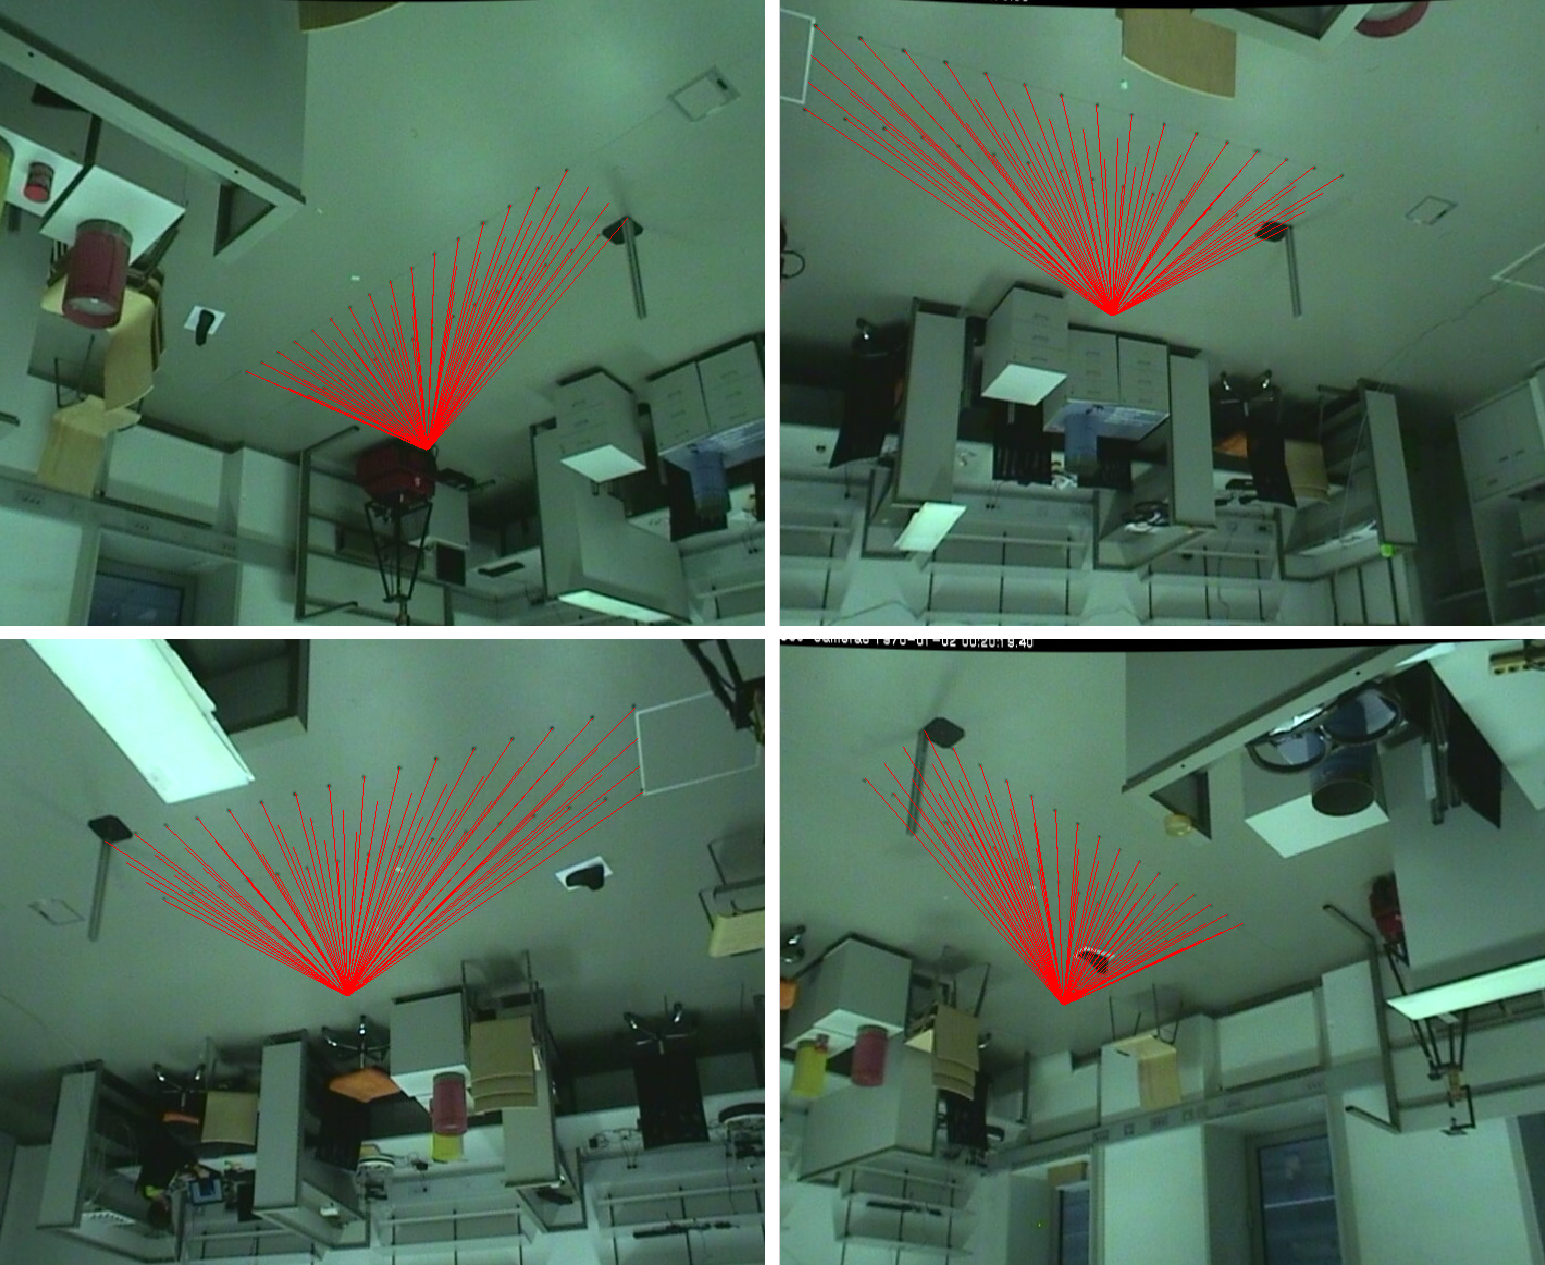
\includegraphics[scale=0.25]{reprojection_corrected.png}
\caption{Na novo ocenjeni zunanji parametri pravilno modelirajo kamere, kar je razvidno iz projekcije piramide.}
\end{figure}

Končna matrika zunanjih parametrov za točke iz tabele \ref{pointpairs} je
\begin{equation}
[R|\vec{T}] = 
\begin{bmatrix}
-0.9544 & 0.3003 & 0.0232 & 106.6226 \\
0.1419 & 0.3877 & 0.9197 & 86.1440 \\
0.2627 & 0.8810 & -0.4127 & -518.2979 
\end{bmatrix}.
\end{equation}

Stolpci rotacijske matrike so le približno paroma ortonormirani, kar je posledica vnašanja napak pri ročnem določanju koordinatnega sistema. Če bi matriko $R$ prisilno ortonormirali, bi s tem vnesli dodatno napako v sistem.

\section{Zaznavanje označevalnika}\label{markersection}
Pri zaznavanju označevalnika je potrebno sliko iz kamere segmentirati. Segmentacija je postopek ločevanja ozadja od objekta zanimanja. Označevalnik ima običajno izrazito drugačno barvo od okolice, zato da pri zaznavanju ne prihaja do dvoumnosti. Segmentacija ponavadi vrne binarno sliko, kjer je ozadje predstavljeno z vrednostjo 0, segmenti pa z vrednostjo 1. 

Segmentiramo lahko tako sivinsko kot barvno sliko. Za vsako točko v sliki se moramo odločiti ali pripada ozadju (0) ali segmentu (1). Vrednost, ki ločuje segmente od ozadja se imenuje prag in se določi na podlagi histograma slike.

Pri segmentiranju barvnih slik se je potrebno odločiti za primeren barvni model. Primarno je barva v slikah predstavljena z modelom RGB (\emph{angl. Red, Green, Blue}). Običajno je bolj primeren model HSV (\emph{angl. Hue, Saturation, Value}) ali HSL (\emph{angl. Hue, Saturation, Lightness}), saj H (ton) komponenta določa barvo neodvisno od njene intenzitete in nasičenosti. Slednja modela sta pri segmentaciji bolj robustna, ker sprememba svetlobe ne vpliva toliko na spremembo tonskega kanala.

Iz segmentirane slike moramo izračunati središče zaznanega objekta (če je prisoten na sliki). To lahko storimo s slikovnimi momenti. Prostorski momenti na sivinski sliki $I$ so definirani kot:
\begin{equation}
M_{ij} = \sum_x \sum_y x^i y^j I(x, y).
\end{equation}

Poznamo še centralne momente, ki so definirani kot:
\begin{align}
\bar{x} &= \frac{M_{10}}{M_{00}} \\
\bar{y} &= \frac{M_{01}}{M_{00}} \\
\mu_{ij} &= \sum_x \sum_y (x - \bar{x})^i (y - \bar{y})^j I(x, y).
\end{align}

Masno središče je predstavljeno z $\bar{x}$ in $\bar{y}$. Moment $M_{00}$ je enak površini segmenta, $M_{10}$ ter $M_{01}$ pa sta vsoti segmenta po $x$ in $y$ koordinatah.

Označevalnik je v osnovi oranžna žogica za namizni tenis. Da pa bi sprememba svetlobe čim manj vplivala na natančnost zazanavanja smo v žogico vgradili modro svetlečo diodo (\emph{angl. LED - Light Emitting Diode}) in stikalo. S pritiskom na stikalo prižgemo označevalnik, da ga kamere lahko zaznajo. Kamere zaznajo žogico kot izrazito rumene barve (slika \ref{markerimg}).

\begin{figure}[H]
\centering
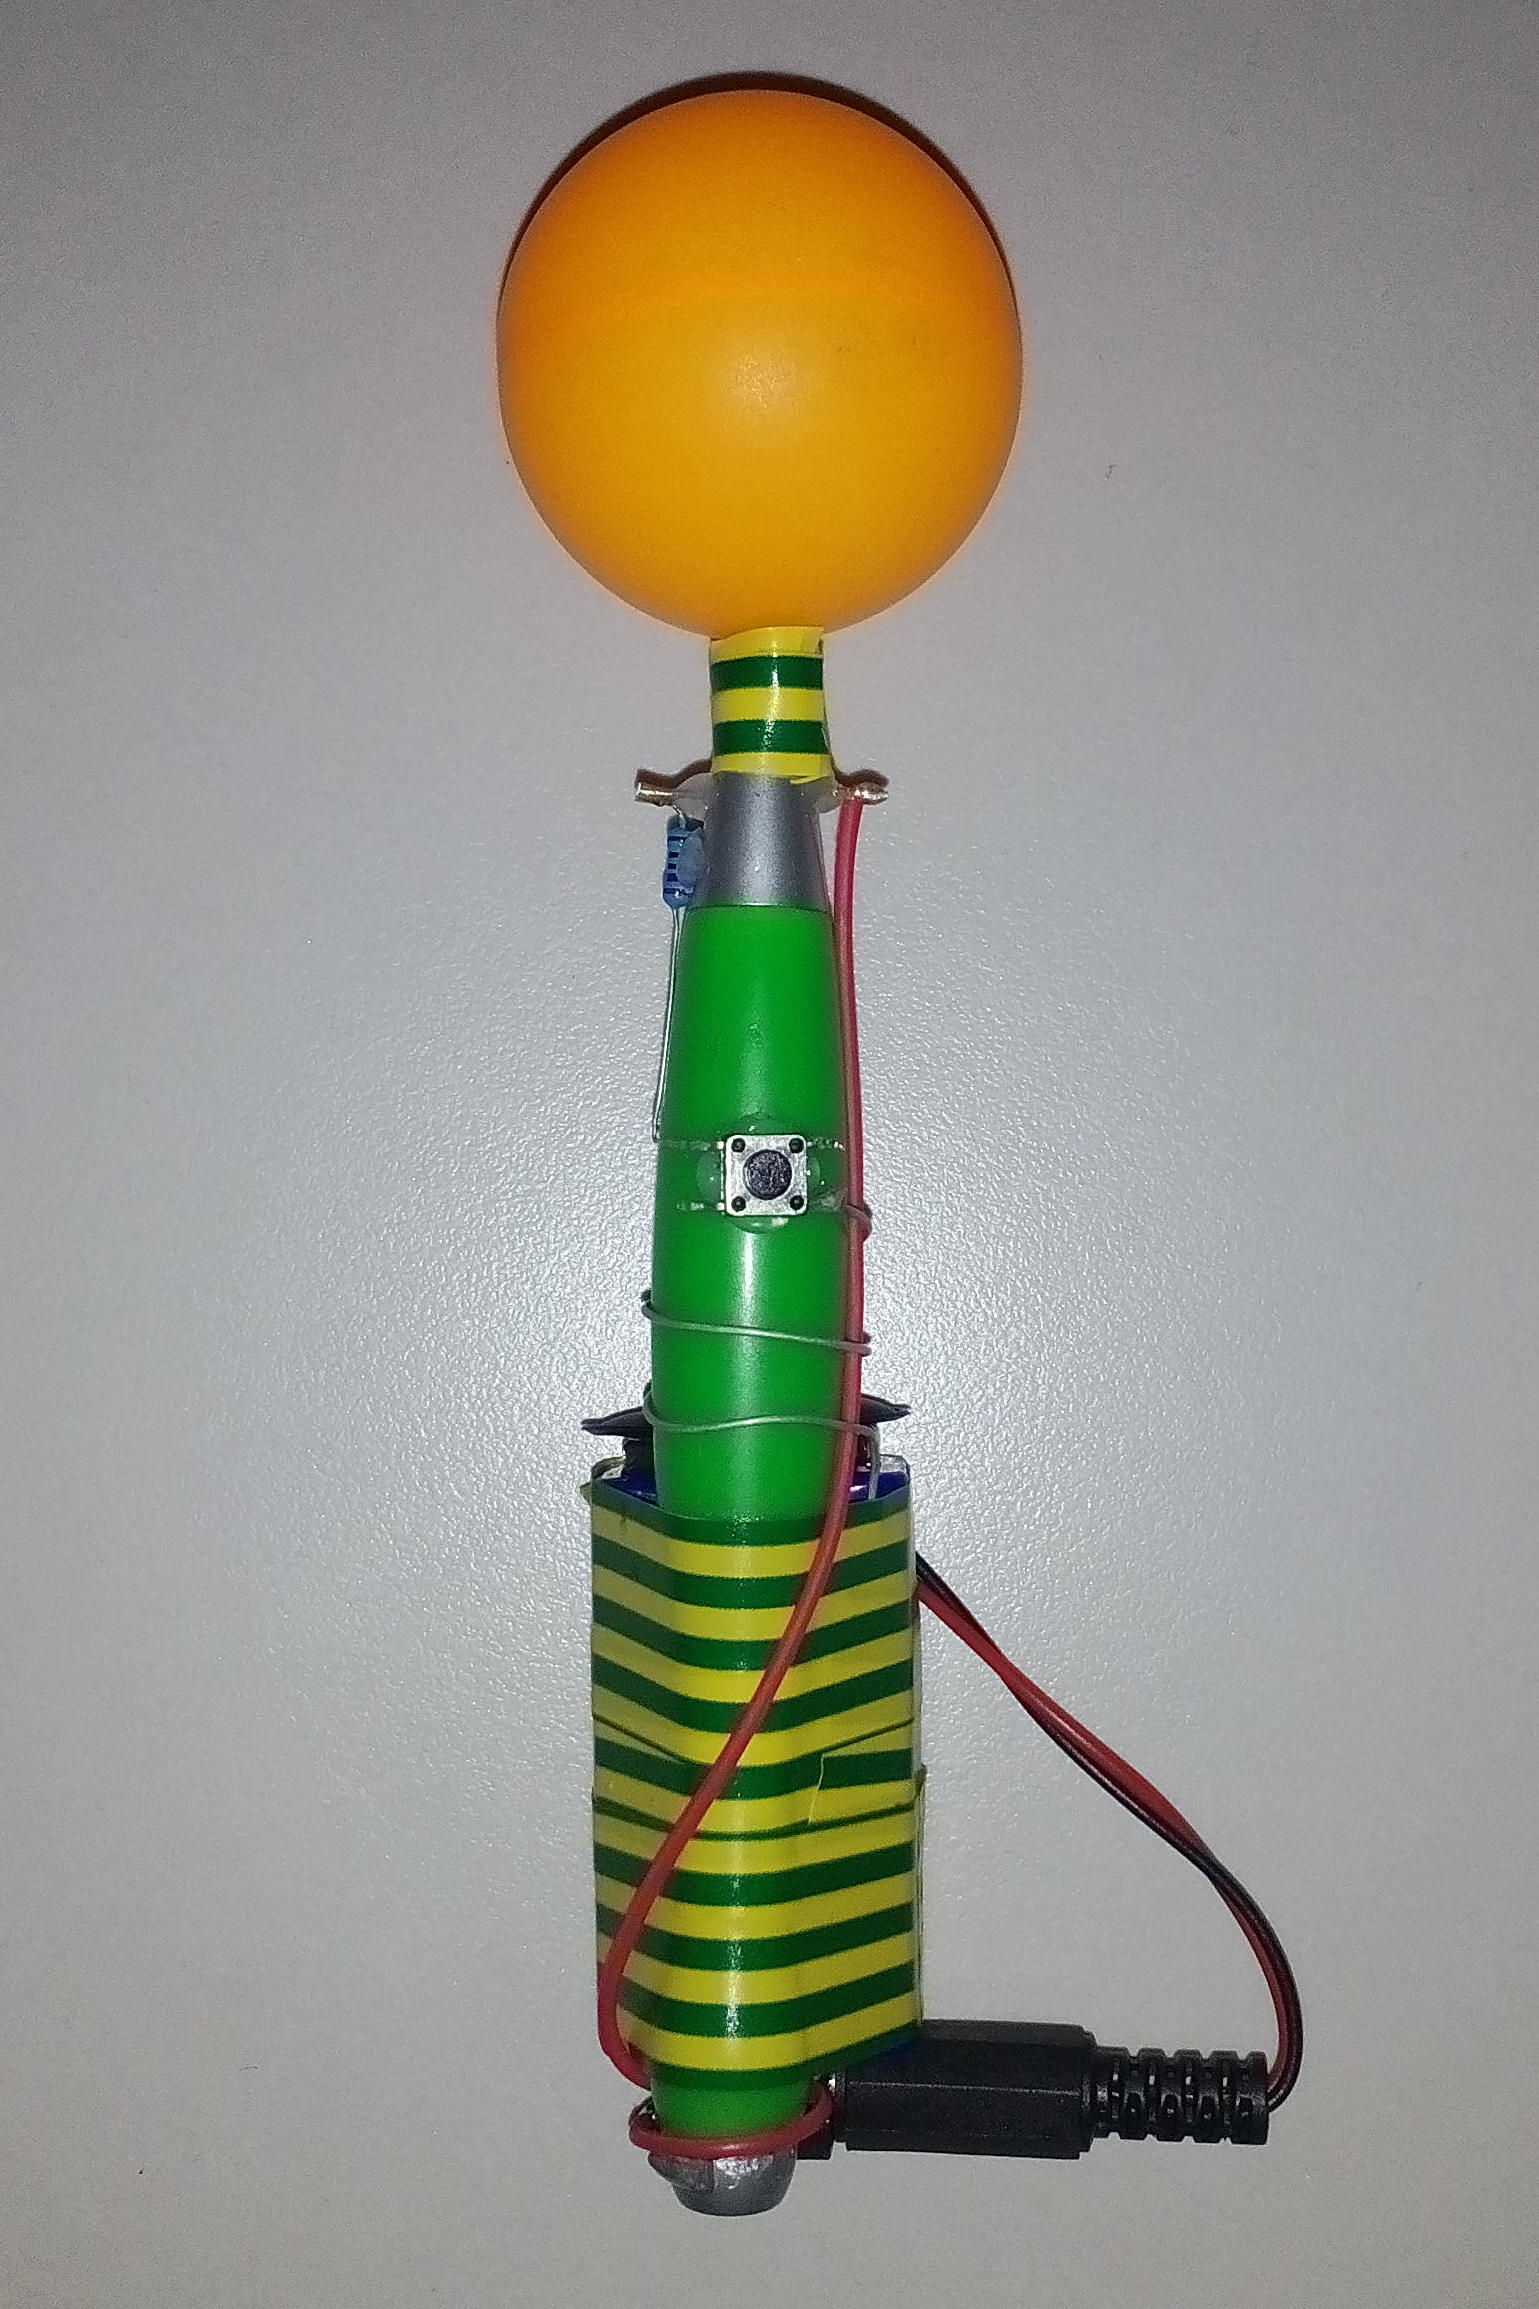
\includegraphics[scale=0.4]{marker_off.png}
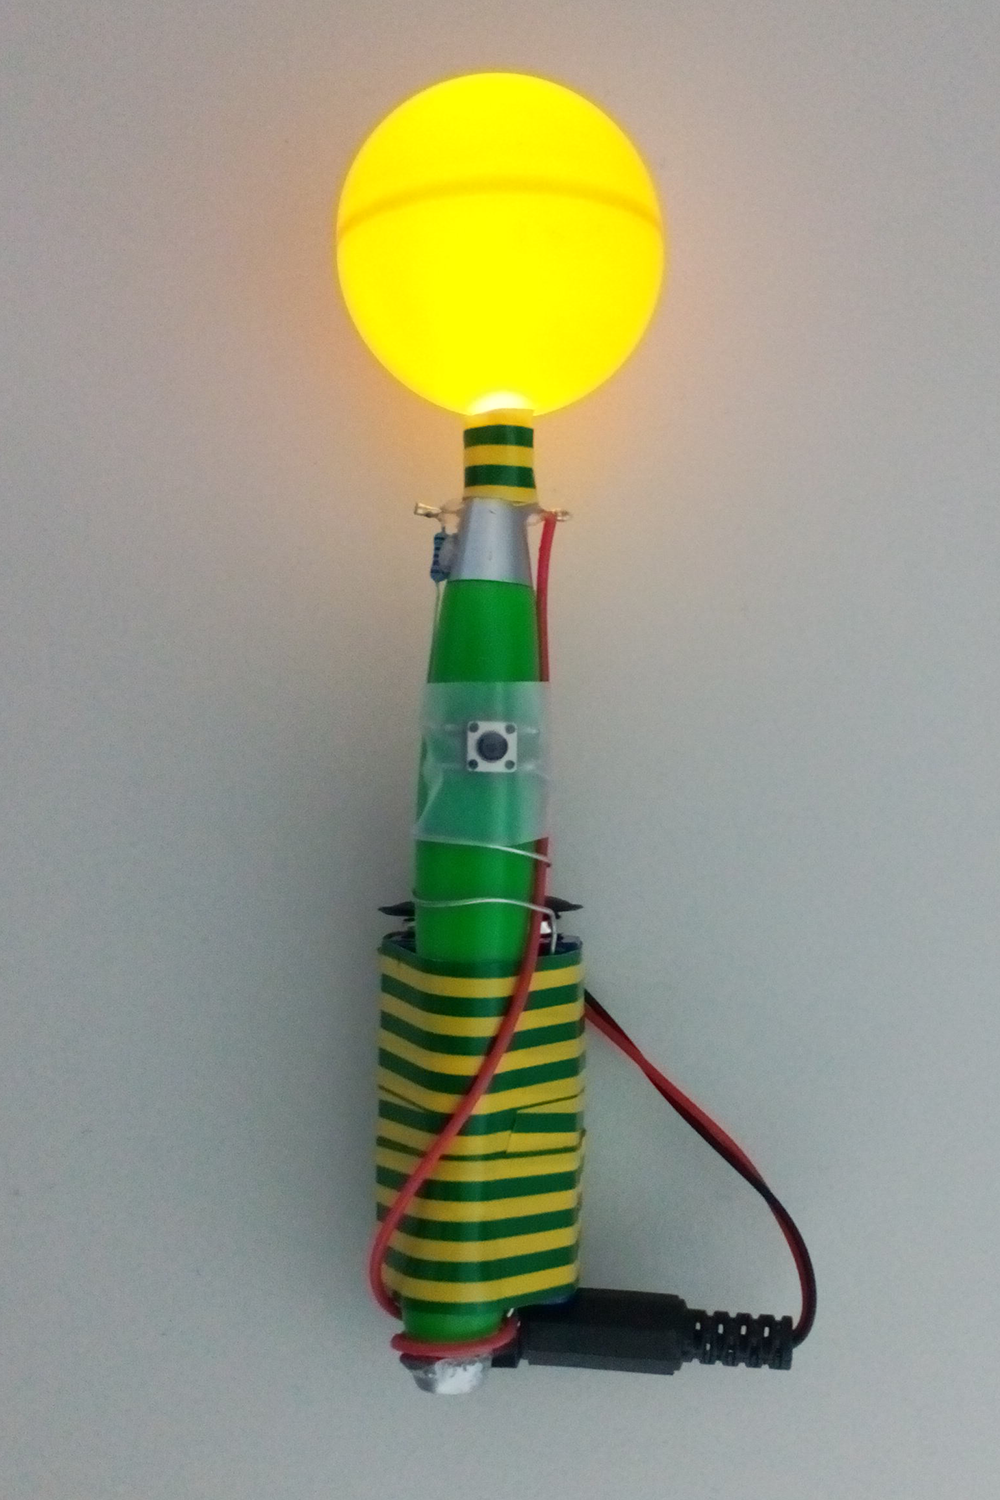
\includegraphics[scale=0.4]{marker_on.png}
\caption{Ugasnjen označevalnik je oranžne barve (levo), prižgan pa izrazito rumene barve (desno).}
\label{markerimg}
\end{figure}

Prag, ki je pravzaprav pas, smo določili z analizo barve slikovnih elementov označevalnika. Za grobo oceno smo vzeli minimalne in maksimalne vrednosti izmerjenih barv. Ker je označevalnik izrazito rumene barve se model RGB izkaže za boljšega kakor model HSV. Interval smo spremenili do te mere, da smo se znebili napačnih detekcij, vendar ohranili natančnost v čim večji meri. Spodnja meja intervala je $[220 \ 220 \ 0]$, zgornja pa $[255, 255, 200]$. V prostoru ne sme prihajati do velikih sprememb v osvetljenosti, zato imajo kamere nastavljen fiksni kontrast, dnevna svetloba pa je izolirana od prostora. Na slikah \ref{segmentedimg} in \ref{detectedimg} sta prikazani posamezni fazi zaznavanja.

\begin{figure}[H]
\centering
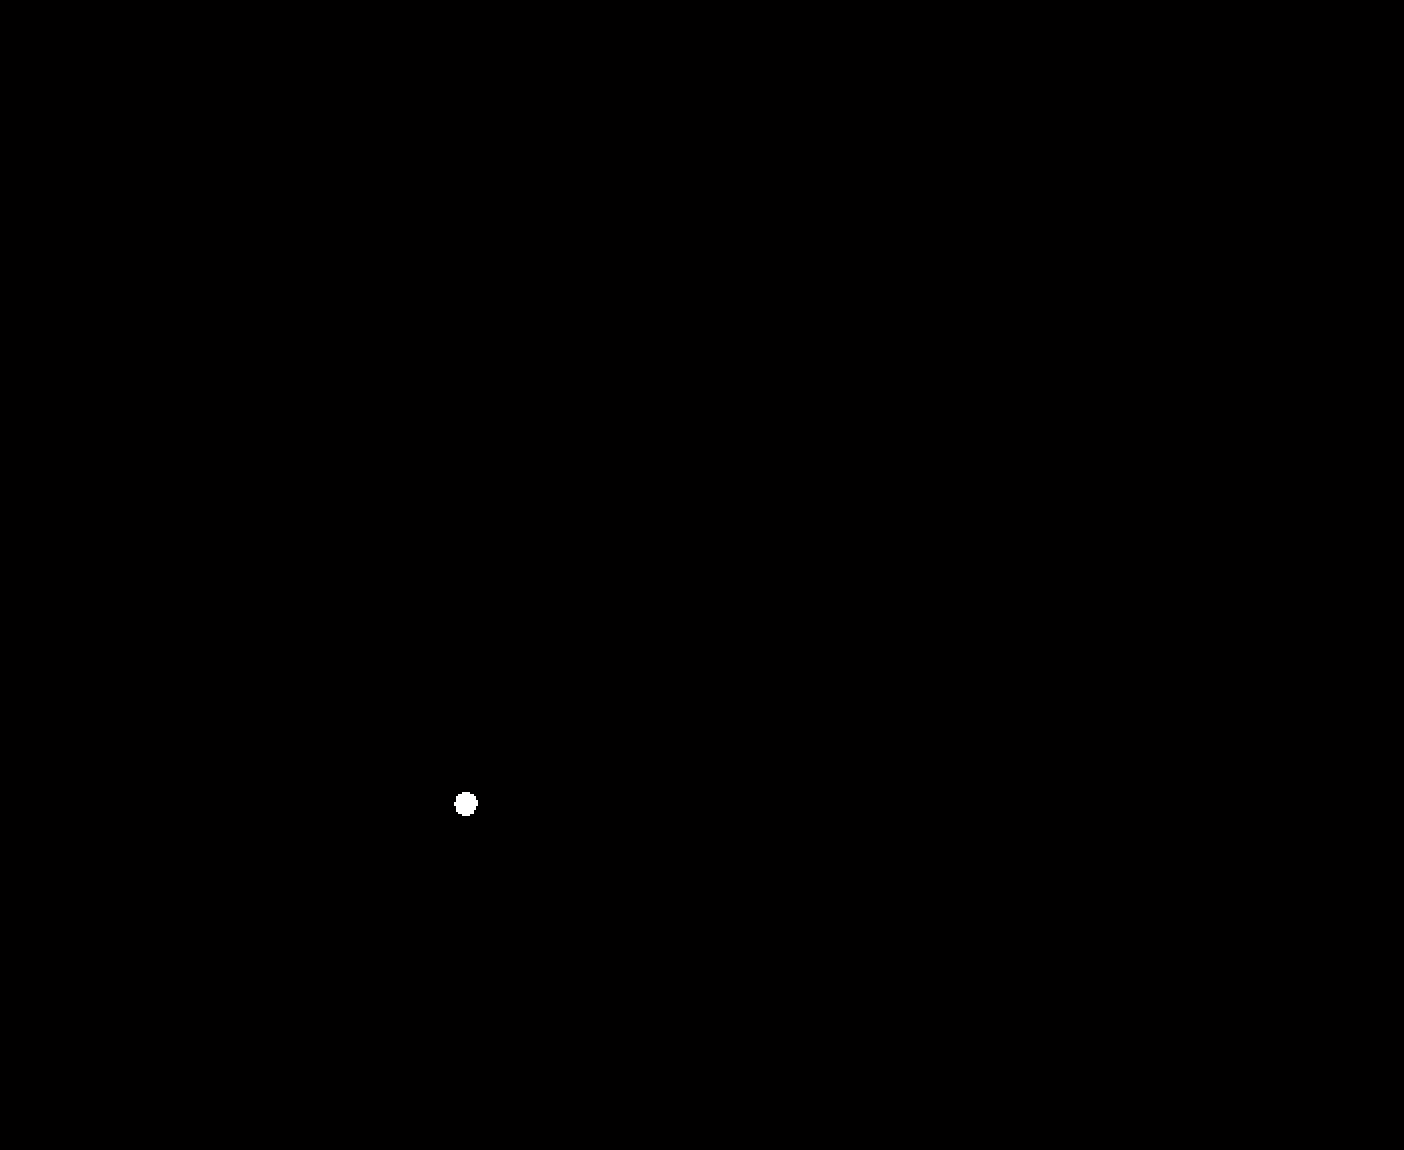
\includegraphics[height=8cm]{segmented.png}
\caption{Segmentacija zajete slike z belo barvo označuje zaznan označevalnik.}
\label{segmentedimg}
\end{figure}

\begin{figure}[H]
\centering
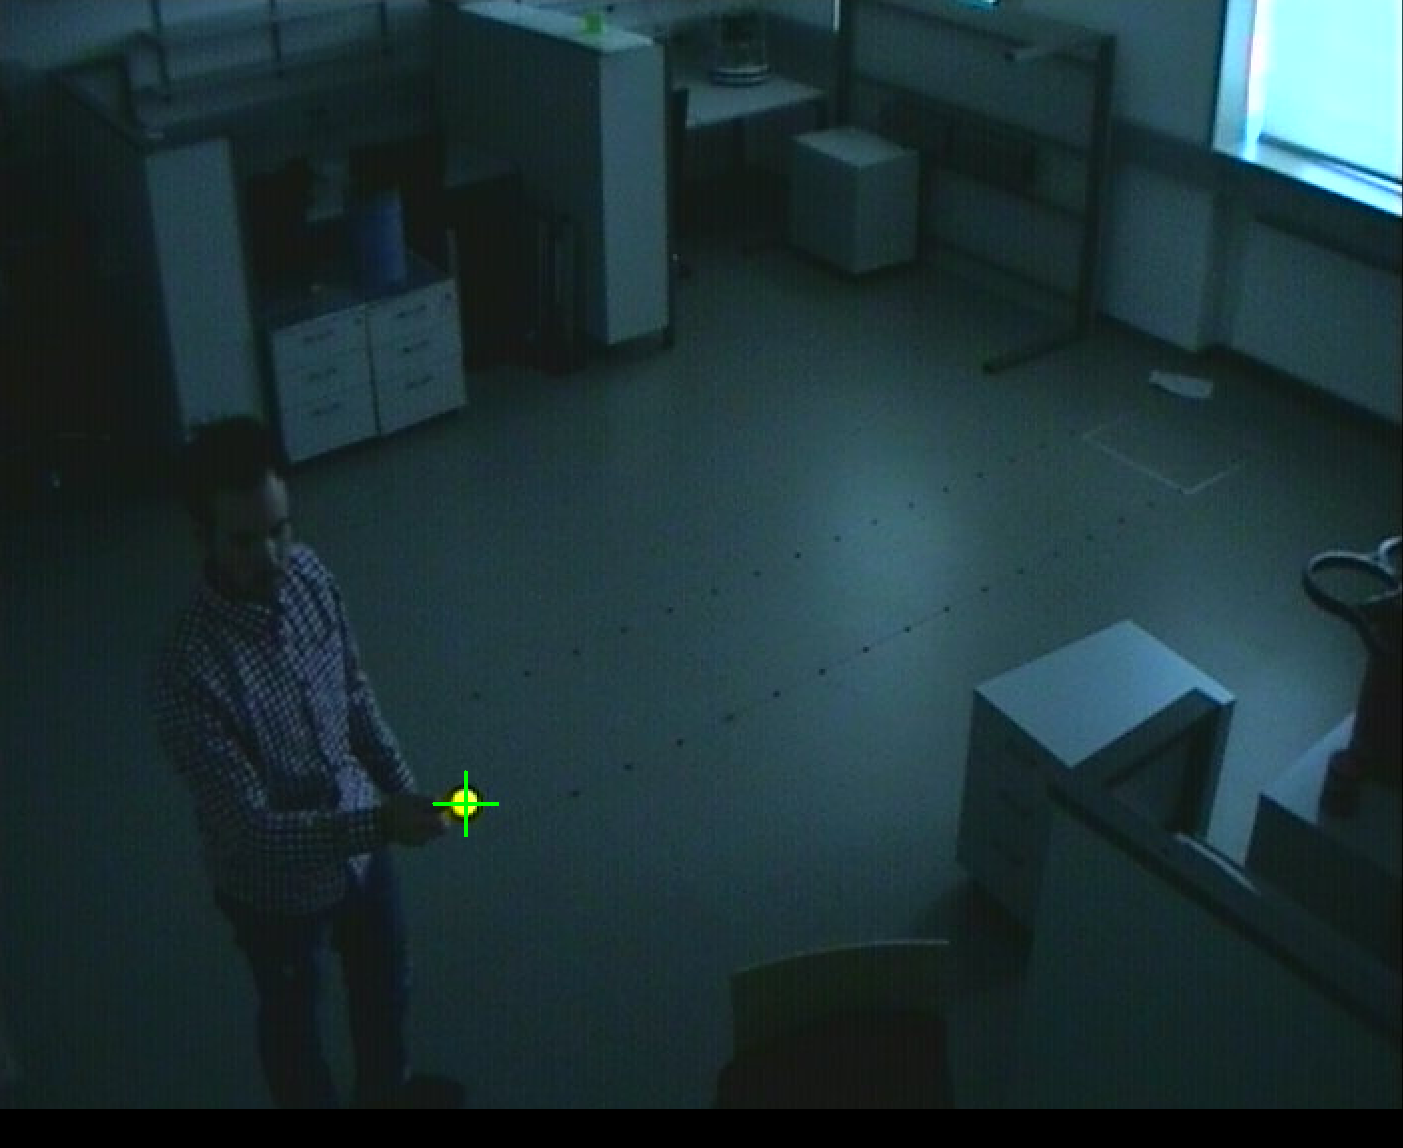
\includegraphics[height=8cm]{detected.png}
\caption{Pozicijo označevalnika na sliki (zeleni +) dobimo z masnim središčem segmenta.}
\label{detectedimg}
\end{figure}

\section{Postavitev sistema}
V prostoru z dimenzijami $7,4 \times 7,7 \times 2,97 \ m^3$ so bile na strop pritrjene štiri Axis 215 PTZ kamere. Sistem deluje v realnem času s 24 meritvami na sekundo. Spodnja slika ilustrira postavitev in orientacijo kamer ter njihovo oštevilčenost.

\begin{figure}[H]
\centering
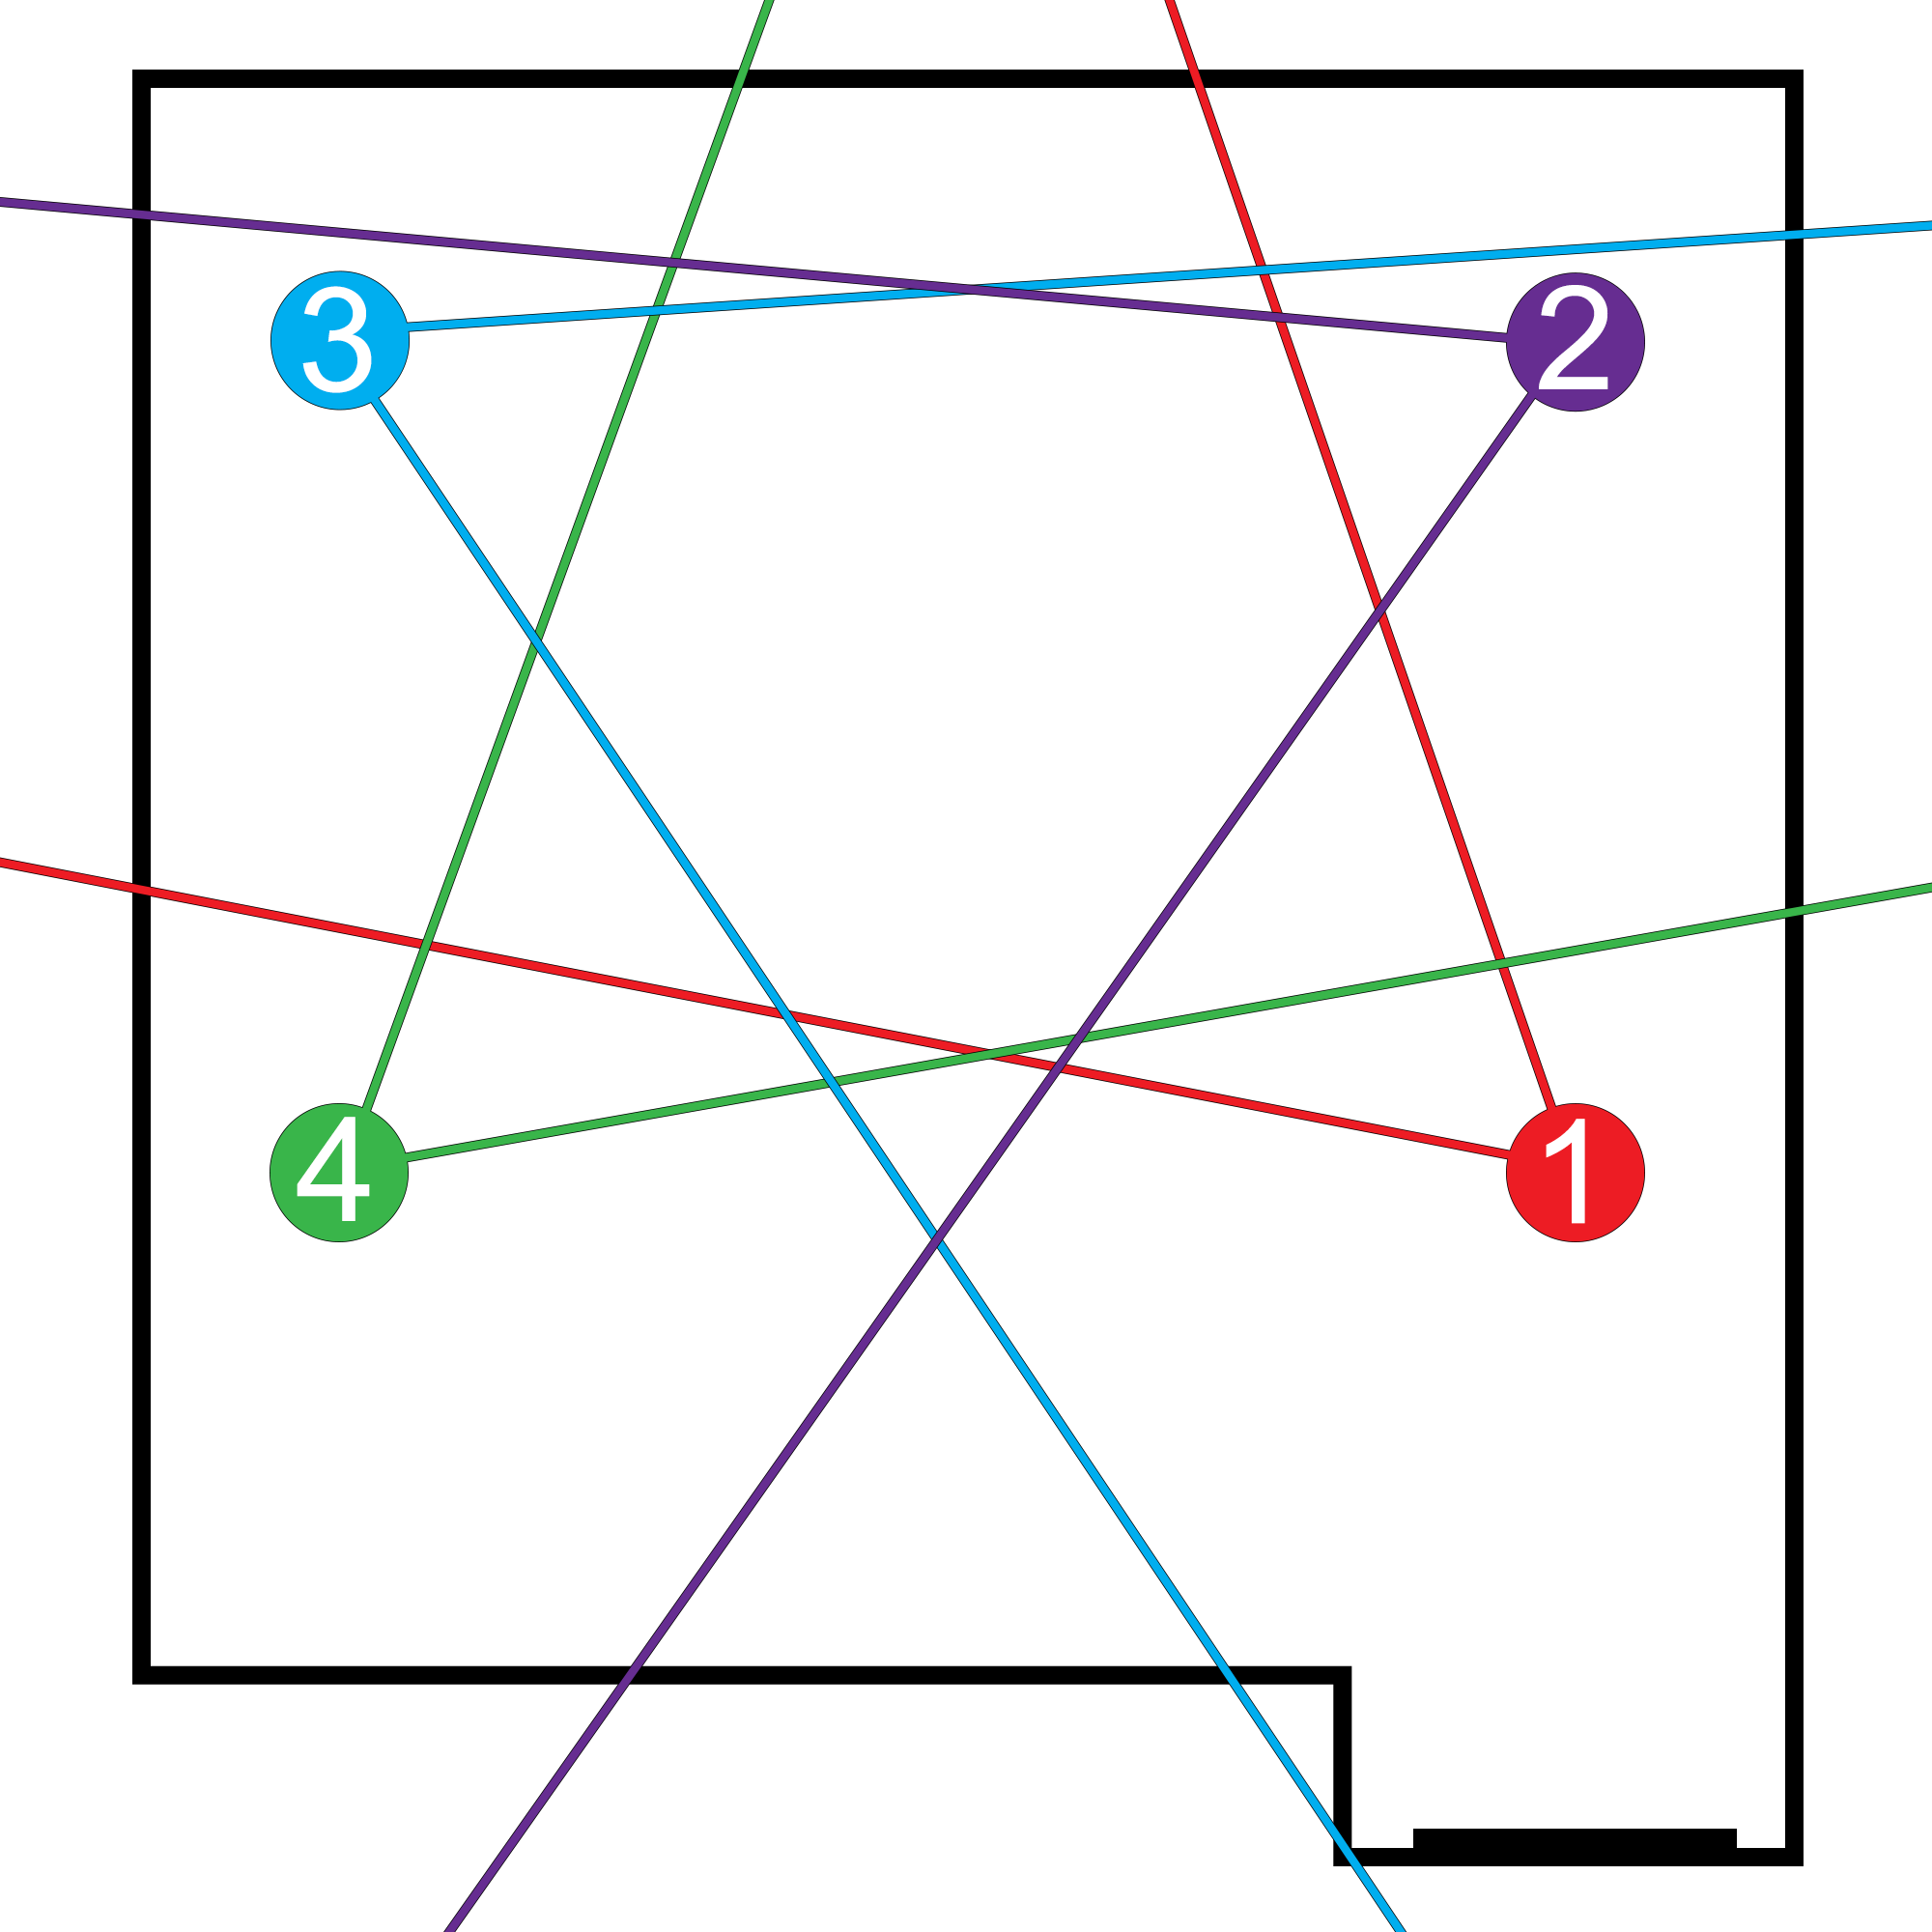
\includegraphics[scale=0.5]{room_setting.png}
\caption{Kamere v prostoru.}
\end{figure}

Kamere so preko omrežja ethernet povezane v zvezdišče in nato v brezžični usmerjevalnik. Prenosni računalnik je v omrežje povezan brezžično. Topologija povezave je predstavljena na sliki \ref{topologyimg}. Na računalniku se izvaja glavni program, ki komunicira s kamerami in računa položaj označevalnika v prostoru. Proces zaznavanja položaja je razdeljen v preproste korake, ki jih opisujeta psevdo kodi \ref{process} in \ref{subprocess}. \\

\begin{algorithm}[H]
 \KwData{parametri in atributi kamere}
 \KwResult{pozicija označevalnika na sliki}
 inicializiraj kamero\;
 \While{True}{
  zajemi sliko iz kamere; \\
  zaznaj označevalnik; \\
  pošlji točko glavnemu procesu; \\
 }
 \caption{Psevdo koda podprocesov, ki zaznavanjo označevalnik na slikah.}
\label{subprocess}
\end{algorithm}
\vspace{1em}
\begin{algorithm}[H]
 \KwData{število kamer n}
 \KwResult{lokacija označevalnika v prostoru}
 zaženi n podprocesov\;
 \While{True}{
 	\ForEach{podproces}{
 		sprejmi točko označevalnika\;
 		dopolni matriko za triangulacijo\;
 	\If{vsaj dve kameri zaznata označevalnik}{
 		trianguliraj položaj označevalnika v prostoru\;
    	izpiši položaj\;
 	}
 }
  zajemi sliko iz kamere\;
  zaznaj označevalnik\;
  pošlji točko glavnemu procesu\;
 }
 \caption{Psevdo koda glavnega procesa, ki lokalizira označevalnik v prostoru.}
\label{process}
\end{algorithm}

\chapter{Eksperimentalni rezultati}
\section{Reprojekcija kalibracijskih točk}\label{reprojectioncalibsection}
Izmeriti želimo kako dobro modeli kamer določajo kalibracijske točke iz tabele \ref{pointpairs}. Pri kalibraciji smo določili pare točk $(X, X')$, kjer je $X$ točka v svetu, $X'$ pa njena projekcija na sliko. S parametri kamere lahko poljubno točko v svetu preslikamo na sliko. Tako lahko točko $X$ projeciramo na sliko in izračunamo reprojekcijsko napako $\vec{e}$, ki je definirana kot:
\begin{equation}
\vec{e} = A[R|\vec{T}]X - X'.
\end{equation} 

\begin{table}
\centering
\begin{tabular}{| l | c | c |}
\hline
kamera & povprečna napaka & varianca napake \\
\hline
1 & 0.8542 & 0.2965 \\
2 & 0.8739 & 0.1146 \\
3 & 0.9786 & 0.6938 \\
4 & 0.8289 & 0.1011 \\
\hline
\end{tabular}
\caption{Povprečna napaka reprojekcije kalibracijskih točk zunanjih parametrov. Napake so merjene v slikovnih elementih.}
\label{errreptab}
\end{table}

\begin{figure}
\centering
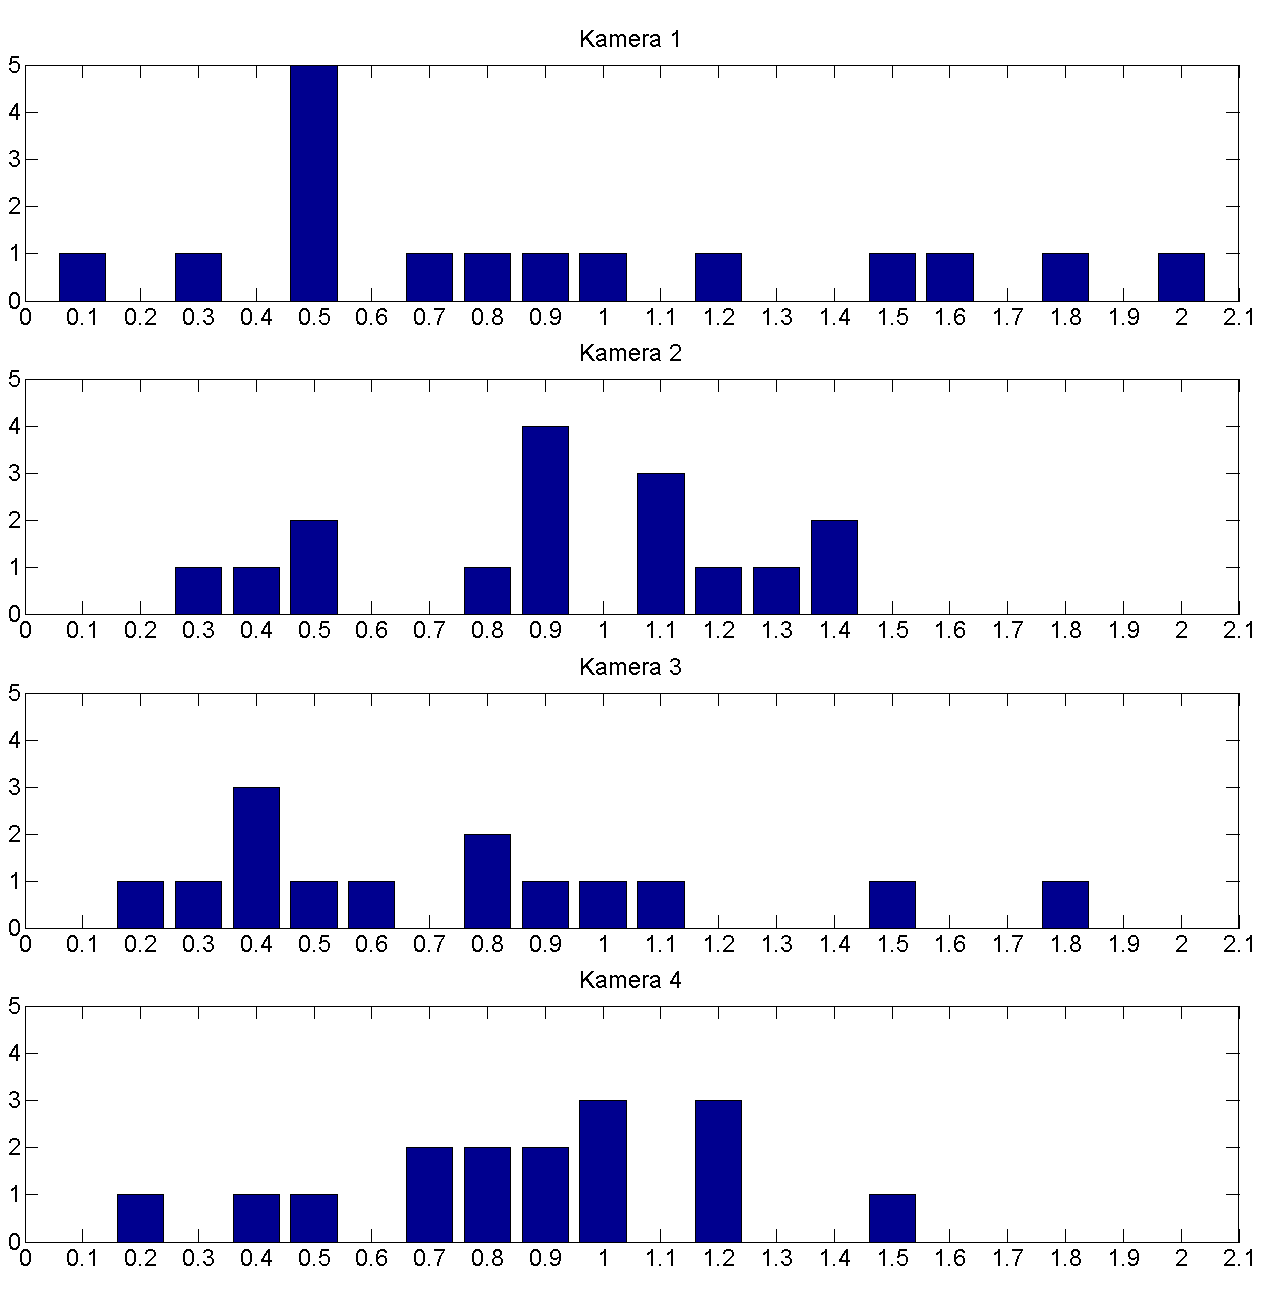
\includegraphics[width=\textwidth,height=\textheight,keepaspectratio]{reprojected_bar.png}
\caption{Histogrami reprojekcijskih napak pri kalibraciji zunanjih parametrov.}
\label{reprojectedbarimg}
\end{figure}

Povprečna reprojekcijska napaka pri kalibriranju notranjih parametrov je med 0.14 in 0.16 slikovnega elementa. To je posledica selektivne izbire slik s katerimi načrtno zmanjšamo napako. Napaka manjša od slikovnega elementa je pri delu s slikami zelo dobra. 

Za kalibracijo zunanjih parametrov, so bile slikovne točke v tabeli \ref{pointpairs} določene ročno z ločljivostjo meritve 1 slikovnega elementa. Pomemben faktor pri tem postopku je vnos človeške napake. Sistem se je kljub napakam kalibriral tako, da je vsota razlik kvadratov najmanjša. V tabeli \ref{errreptab} in na sliki \ref{reprojectedbarimg} opazimo, da so povprečne napake dokaj konsistentne pri okoli $0,9$ slikovnega elementa. Pri tretji kameri izstopa varianca, kar je najverjetneje posledica manj natančnega ročnega določanja točk.

\section{Natančnost zaznavanja označevalnika}
Natančnost zaznavanja označevalnika lahko izmerimo tako, da primerjamo zaznano točko s točno (resnično) točko označevalnika (slika \ref{mdetectioneximg}). Formalno to zapišemo kot:
\begin{equation}
\vec{e} = \vec{x}_{zaznana} - \vec{x}_{tocna}.
\end{equation}

Natančnost izmerimo na dveh vrstah množic. Prva ima na vseh slikah statično pozicijo označevalnika, saj je bil v času zajemanja slik označevalnik na istem mestu v prostoru. Zaradi šuma pri zajemu slik pa algoritem za zaznavanje označevalnika ne zazna vedno enake točke na sliki. Druga vrsta množice pa vsebuje slike, ki prikazujejo označevalnik vsakič na drugem mestu v prosotru (je dinamičen). Vsaka množica vsebuje okoli 100 slik, po 25 iz vsake kamere. Slike na katerih označevalnik ni viden so bile odstranjene iz množice (20 odstranjenih slik iz dinamične množice). Točne točke označevalnika so bile določene ročno z ločljivostjo 1 slikovnega elementa, ker MATLAB-ovo orodje za označevanje točk ne dovoljuje večje natančnosti. 
\begin{figure}[H]
\centering
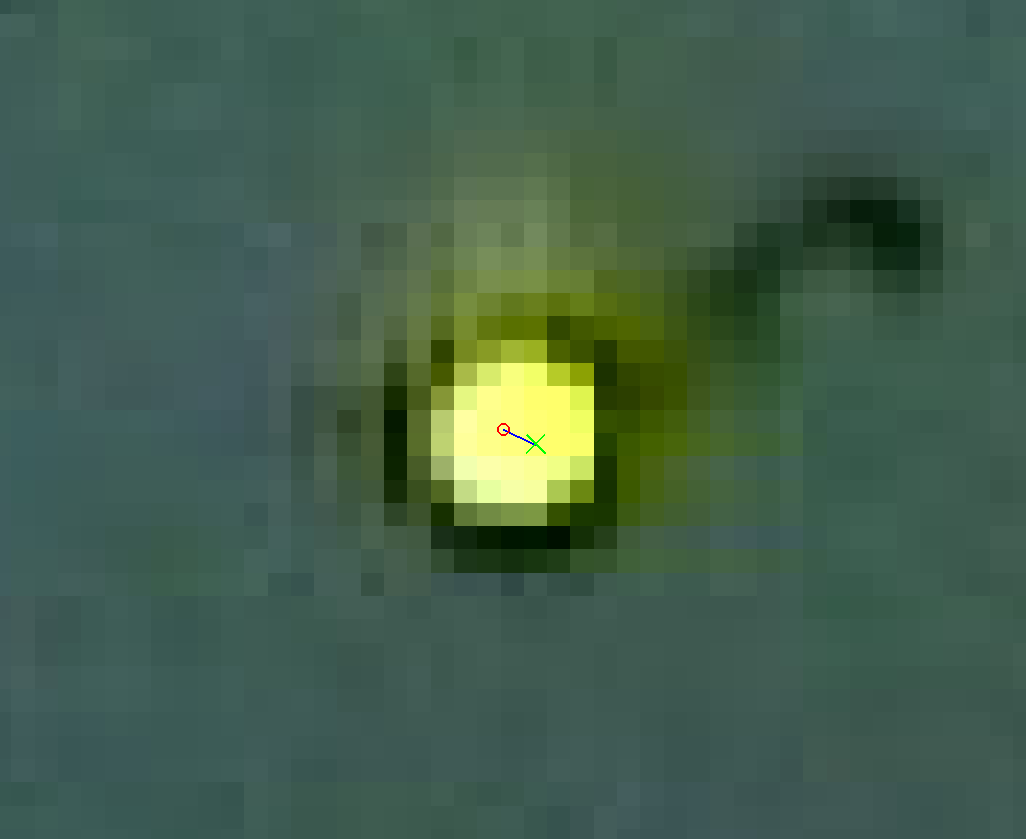
\includegraphics[width=\textwidth,height=\textheight,keepaspectratio]{marker_detection_example.png}
\caption{Resnična točka je označena z rdečo krožnico, zaznana pa z zelenim križem. Vektor napake je predstavljen z modro daljico.}
\label{mdetectioneximg}
\end{figure}

\begin{figure}
\centering
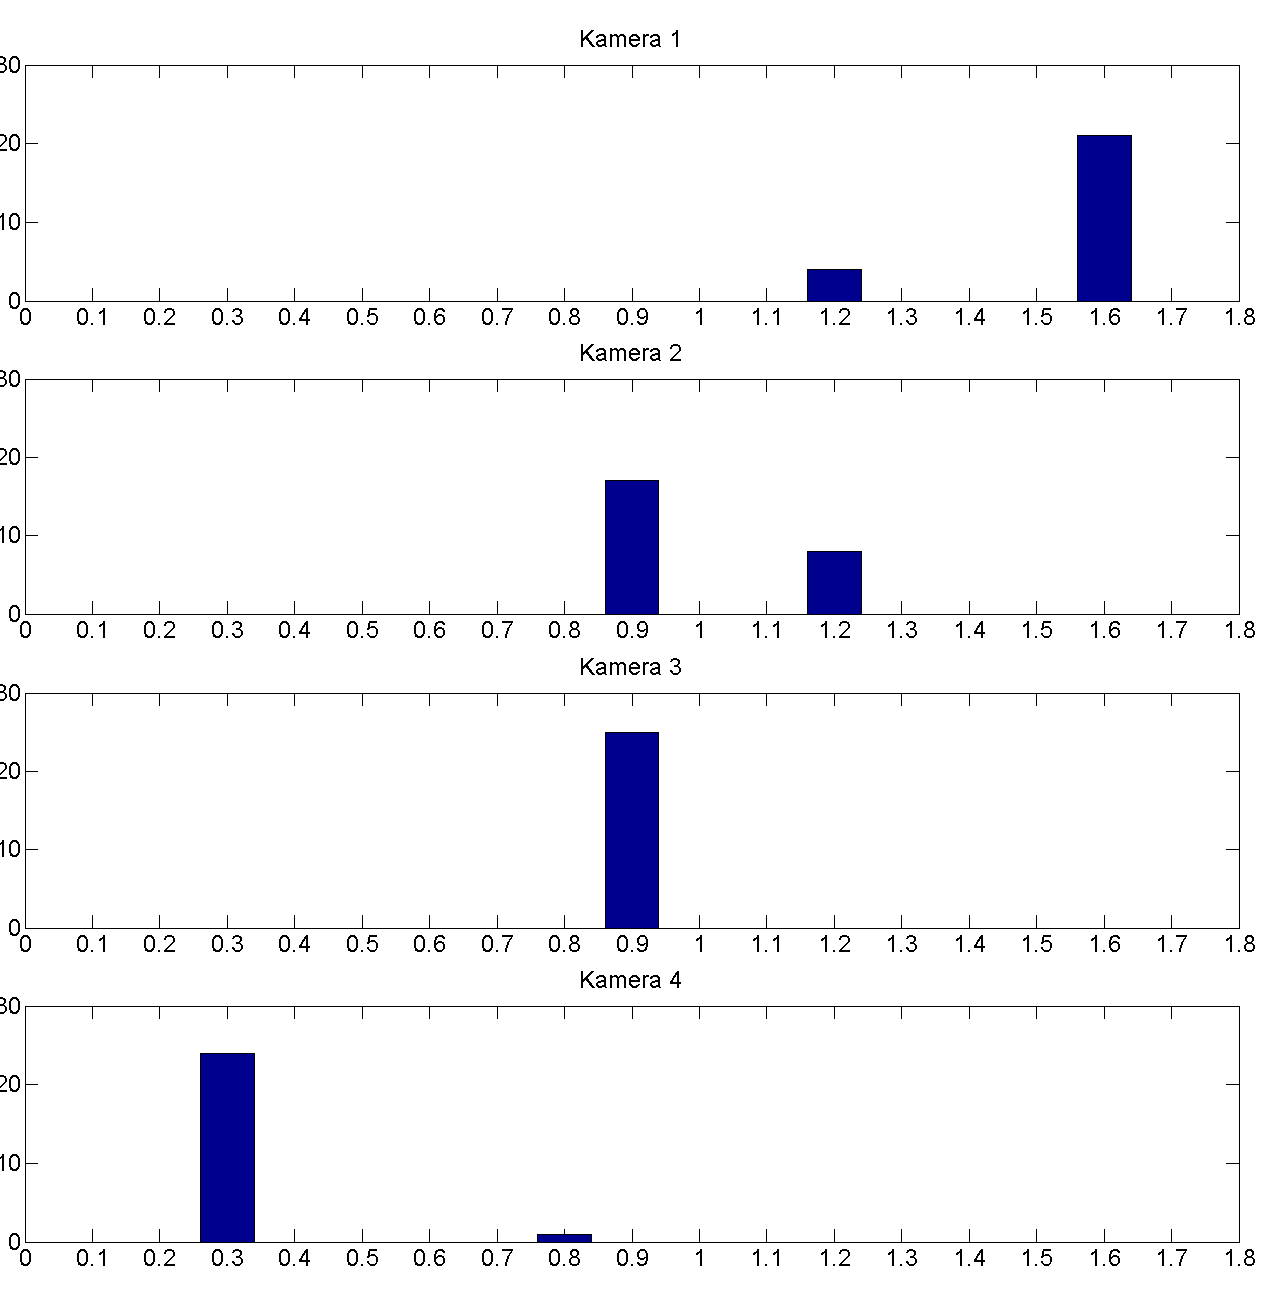
\includegraphics[width=\textwidth,height=\textheight,keepaspectratio]{marker_detection_static_bar.png}
\caption{Histogrami napak zaznavanja statičnega označevalnika.}
\label{marker_detection_static_bar}
\end{figure}

\begin{figure}
\centering
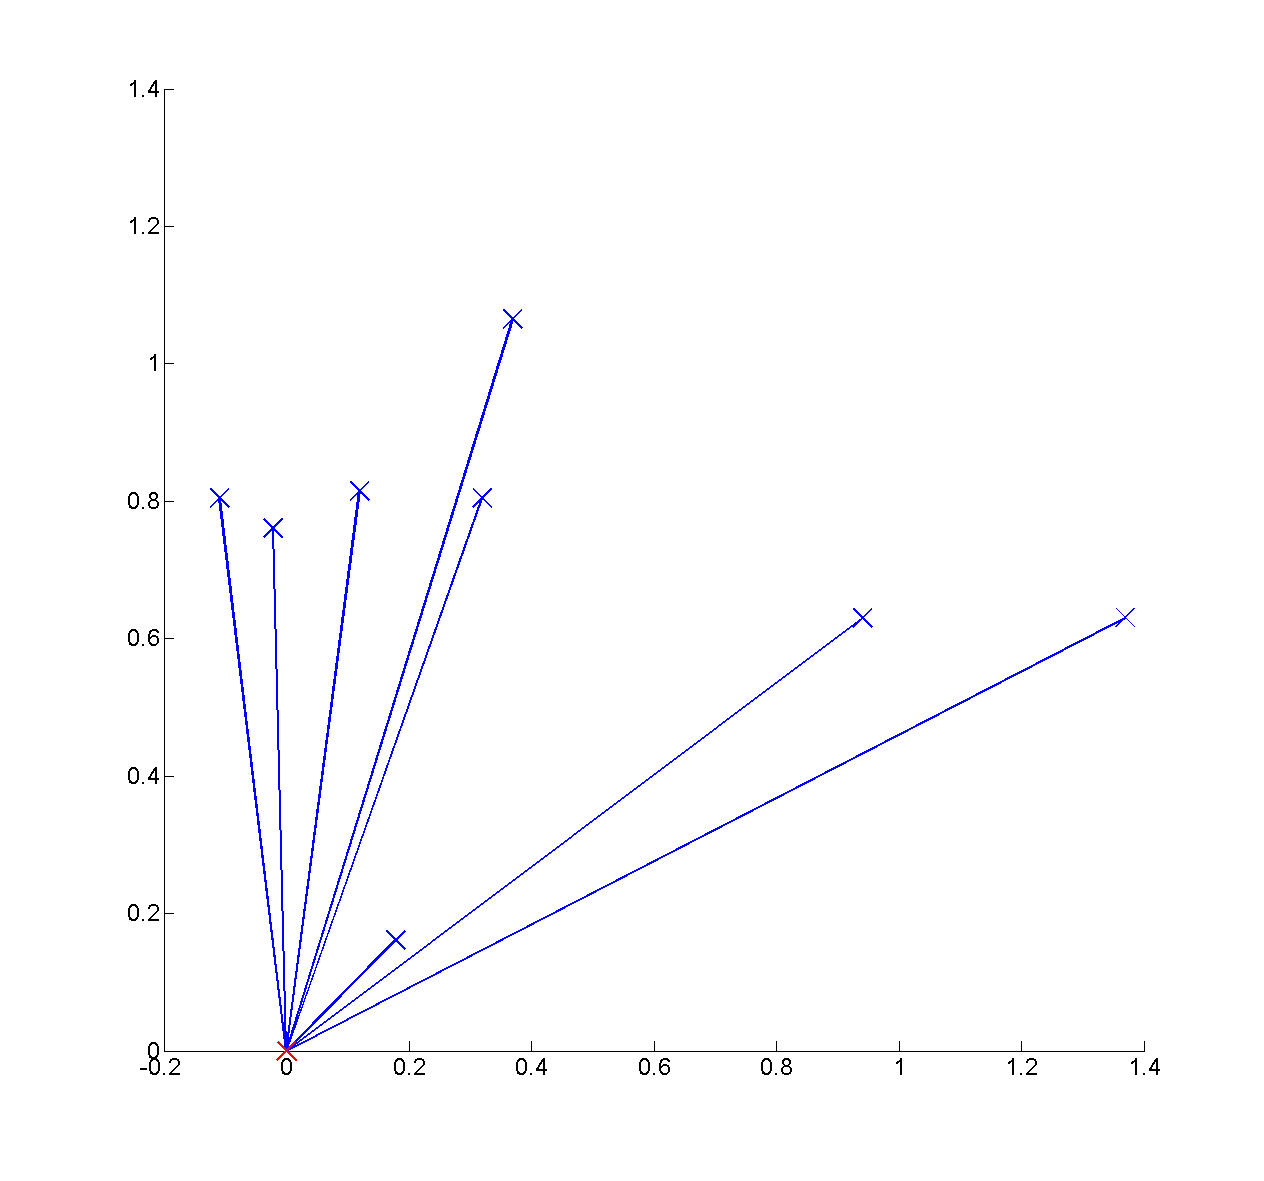
\includegraphics[width=\textwidth,height=\textheight,keepaspectratio]{marker_detection_static_errors.png}
\caption{Graf vektorjev napak v statični množici. Vektorji so usmerjeni predvsem v prvi kvadrant.}
\label{marker_detection_static_errors}
\end{figure}

\begin{figure}
\centering
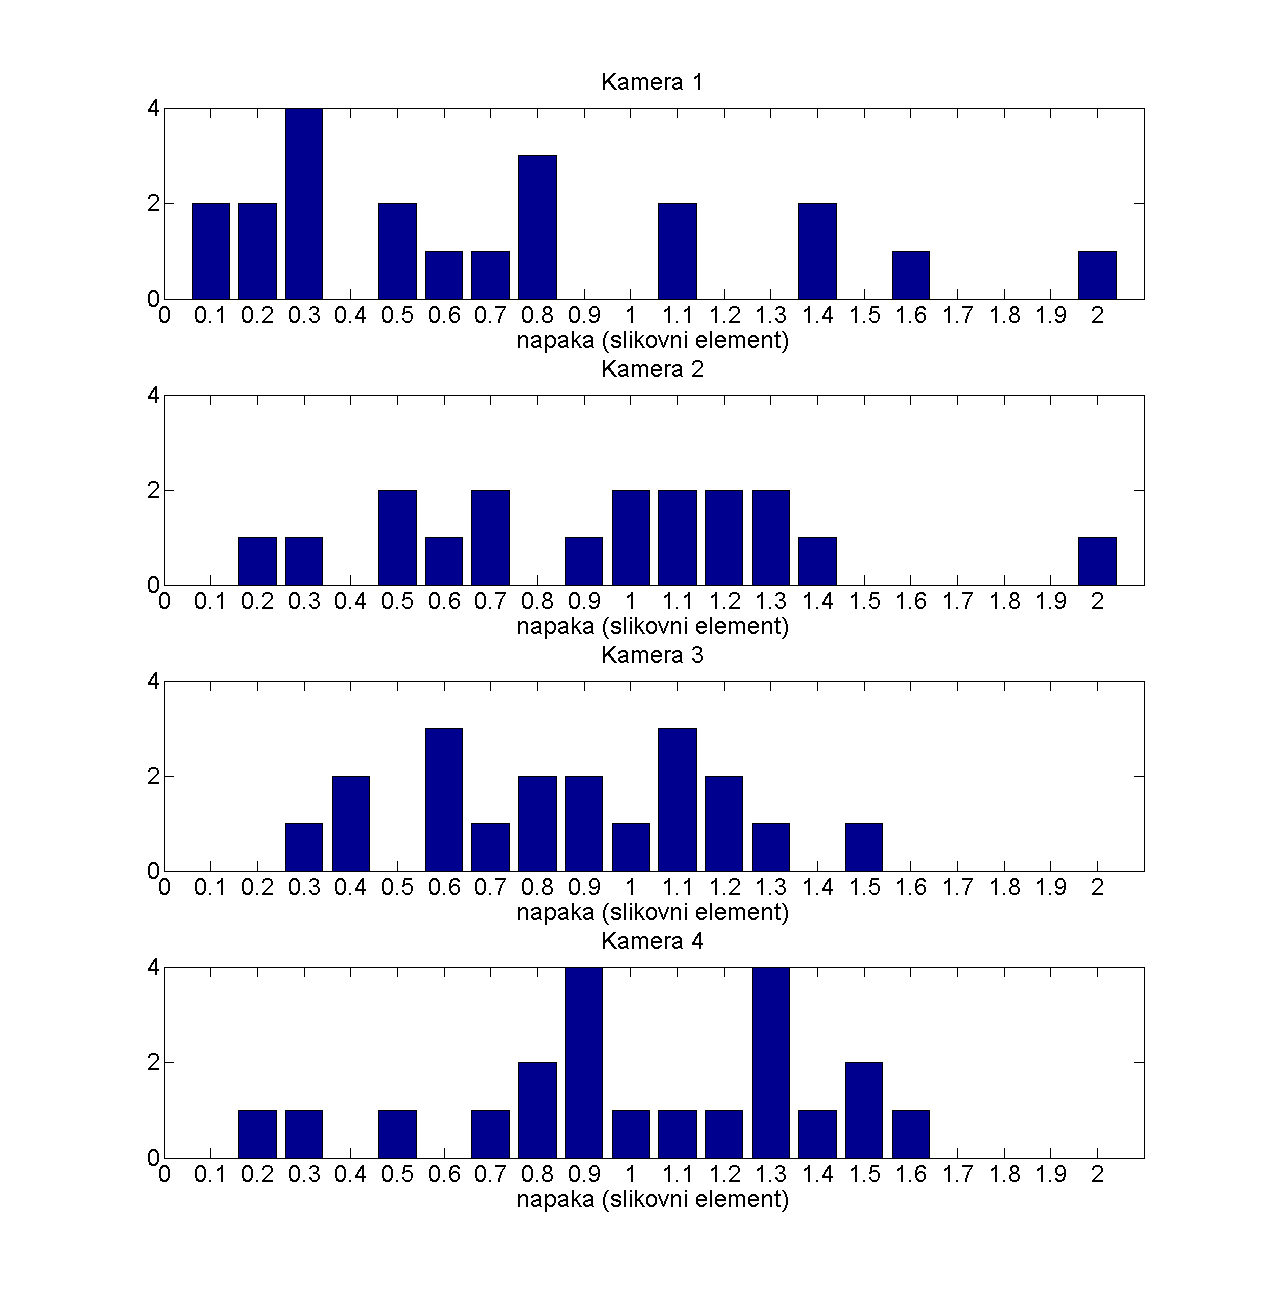
\includegraphics[width=\textwidth,height=\textheight,keepaspectratio]{marker_detection_dynamic_bar.png}
\caption{Histogrami napak zaznavanja dinamičnega označevalnika.}
\label{marker_detection_dynamic_bar}
\end{figure}

\begin{figure}
\centering
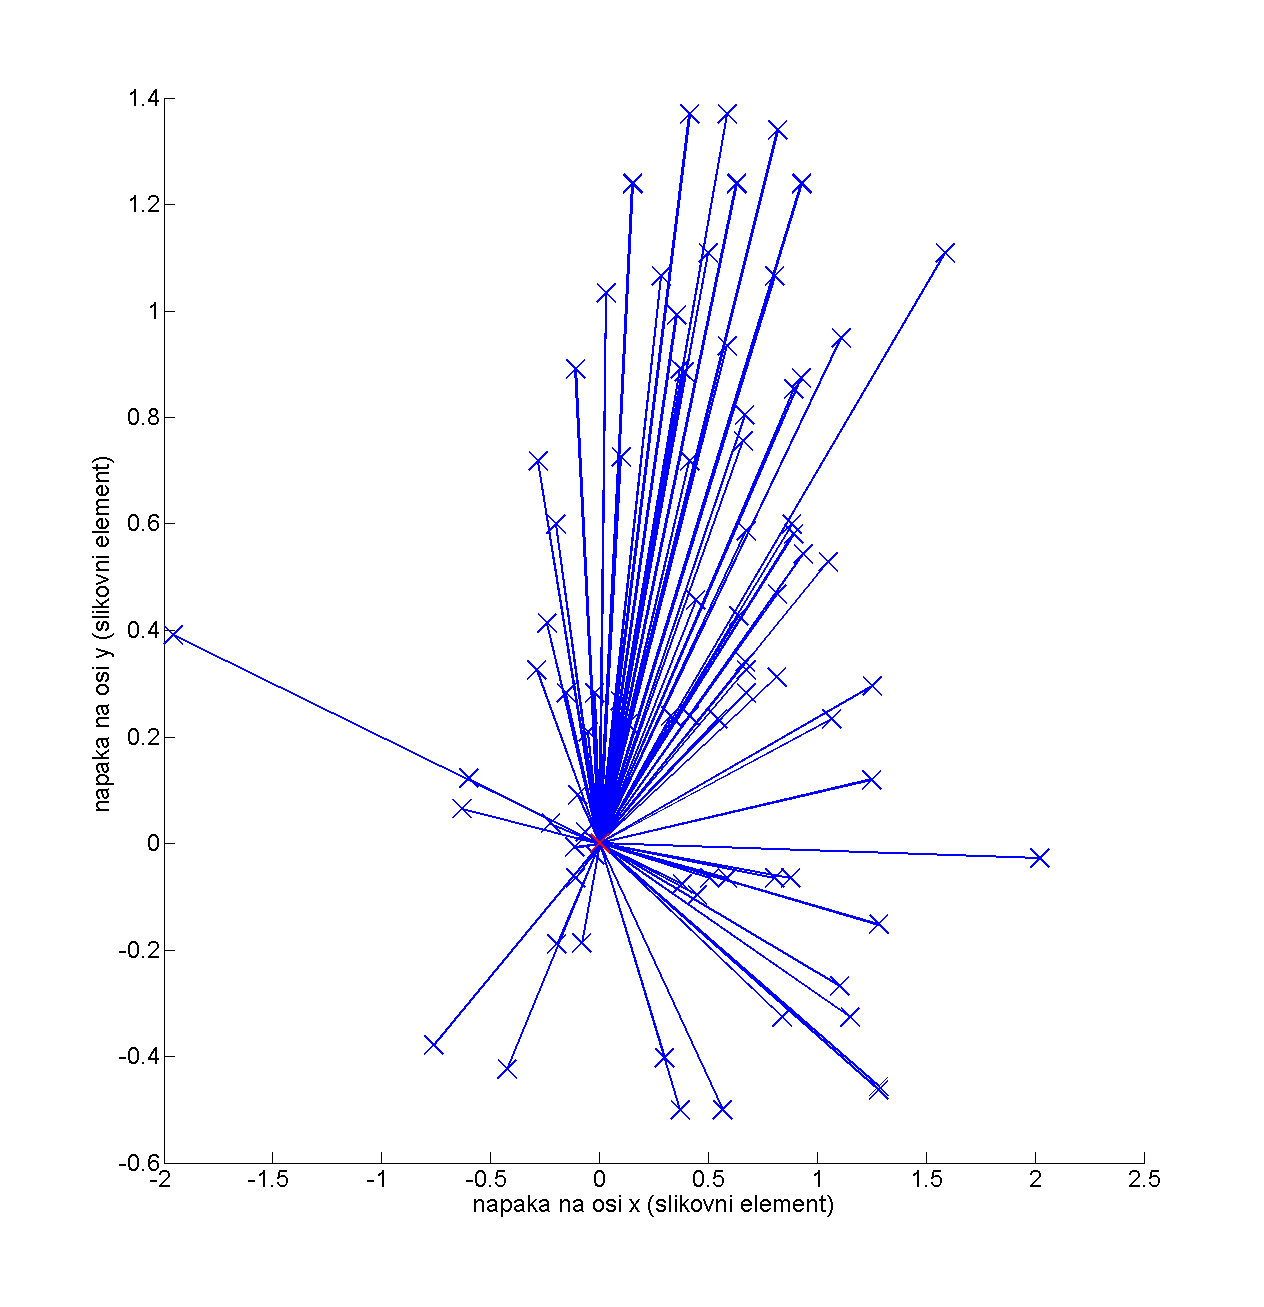
\includegraphics[width=\textwidth,height=\textheight,keepaspectratio]{marker_detection_dynamic_errors.png}
\caption{Graf vektorjev napak v dinamični množici. Gostota zaznanih točk je večja v zgornji polovici grafa, kar je najverjetneje posledica rahle neenakomerne osvetljenosti označevalnika.}
\label{marker_detection_dynamic_errors}
\end{figure}

Povprečje napake v prvi množici (statični) je $0,8614$ slikovnega elementa z varianco $0,1899$. Iz histogramov na sliki \ref{marker_detection_static_bar} se lepo vidi, da je varianca majhna. Slike iz tretje in četrte kamere skoraj vedno določijo enako točko označevalnika. Pri slikah iz prve in druge kamere pa šum povzroči majhno spremembo intenzitet pik, kar posledično zmede algoritem za zaznavanje označevalnika.

Povprečje napake v drugi množici (dinamični) je $0,852$ slikovnega elementa z varianco $0,2124$. Iz histogramov na sliki \ref{marker_detection_dynamic_bar} vidimo, da je napaka bolj enakomerno porazdeljena kot pri zaznavanju statičnega označevalnika.

Vektorji napak na slikah \ref{marker_detection_static_errors} in \ref{marker_detection_dynamic_errors} pa so bolj gosto porazdeljeni v prvem kvadrantu. V času meritev je bila v prostoru prisotna usmerjena svetloba, ki je povzročila rahlo neenakomerno osvetlitev označevalnika.

\section{Natančnost lokalizacije}
Natančnost lokalizacije določimo tako, da na izbrane poljubne točke v prostoru postavimo označevalnik in trianguliramo njegovo lokacijo. Dobljeno pozicijo primerjamo z izbrano in tako dobimo napako $\vec{e}$.
\begin{equation}
\vec{e} = \vec{X}_{trianguliran} - \vec{X}_{tocen}
\end{equation}

Zunanji parametri kamer so bili kalibrirani s 16 koplanarnimi točkami v svetu (tabela \ref{pointpairs}). Za testiranje natančnosti lokaliziranja pa izberemo osem točk, prikazanih v tabeli \ref{measuringptstab}. Napake izračunamo pri triangulaciji točk z dvemi, tremi in štirimi kamerami. Izbrane točke so vizualizirane v prostoru na sliki \ref{accuracy_points}.

\begin{table}[H]
\centering
\begin{tabular}{| c | c | c |}
\hline
x ($cm$) & y ($cm$) & z ($cm$) \\
\hline
0 & 40 & 76 \\
0 & 80 & 76 \\
40 & 40 & 76 \\
40 & 80 & 76 \\
80 & 40 & 76 \\
80 & 80 & 76 \\
120 & 40 & 76 \\
120 & 80 & 76 \\
\hline
\end{tabular}
\caption{Referenčne točke za meritve v prostoru.}
\label{measuringptstab}
\end{table}

\begin{figure}
\centering
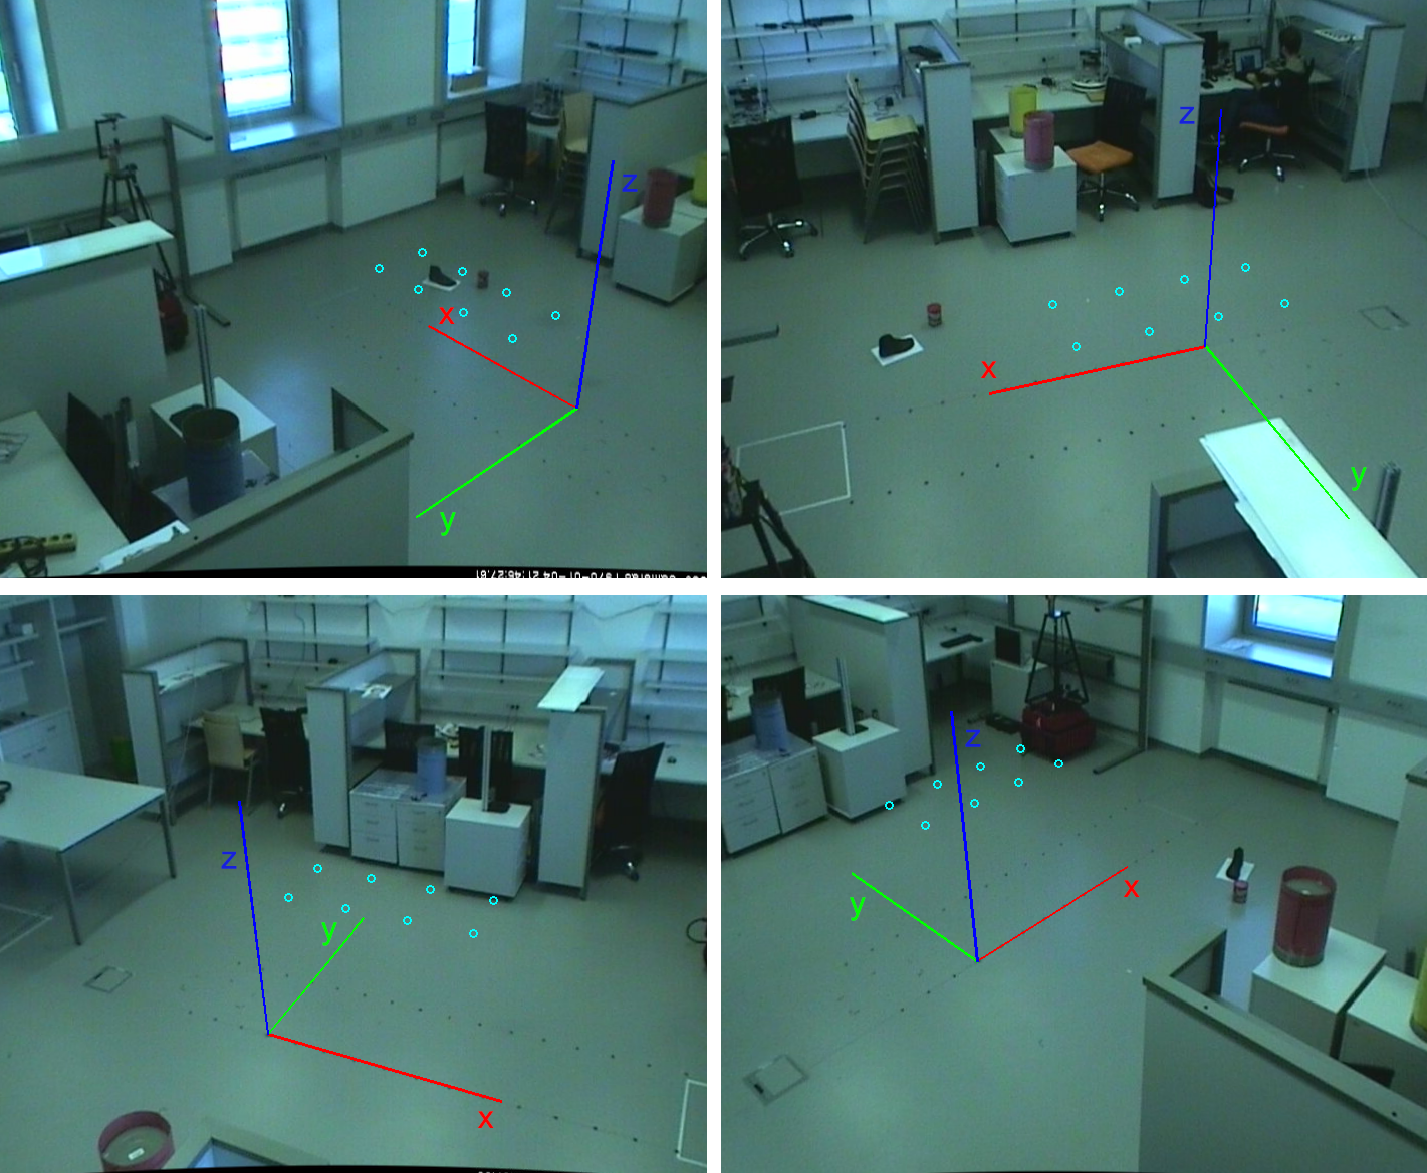
\includegraphics[width=\textwidth,height=\textheight,keepaspectratio]{accuracy_points.png}
\caption{Izbrane točke so predstavljene s krogci. Vektorji x, y in z označujejo koordinatni sistem prostora.}
\label{accuracy_points}
\end{figure}

\begin{table}
\centering
\begin{tabular}{| c | c | c | c |}
\hline
št. kamer & št. meritev & povprečna napaka ($cm$) & varianca napake ($cm^2$)  \\
\hline
2 & 272 & 6,4854 & 2,6562 \\
3 & 408 & 2,5539 & 1,1009 \\
4 & 712 & 4,4618 & 0,2218 \\
\hline
\end{tabular}
\caption{Povprečna napaka pri pozicioniranju z dvemi, tremi in štirimi kamerami.}
\label{positionerrortable}
\end{table}

\begin{figure}
\centering
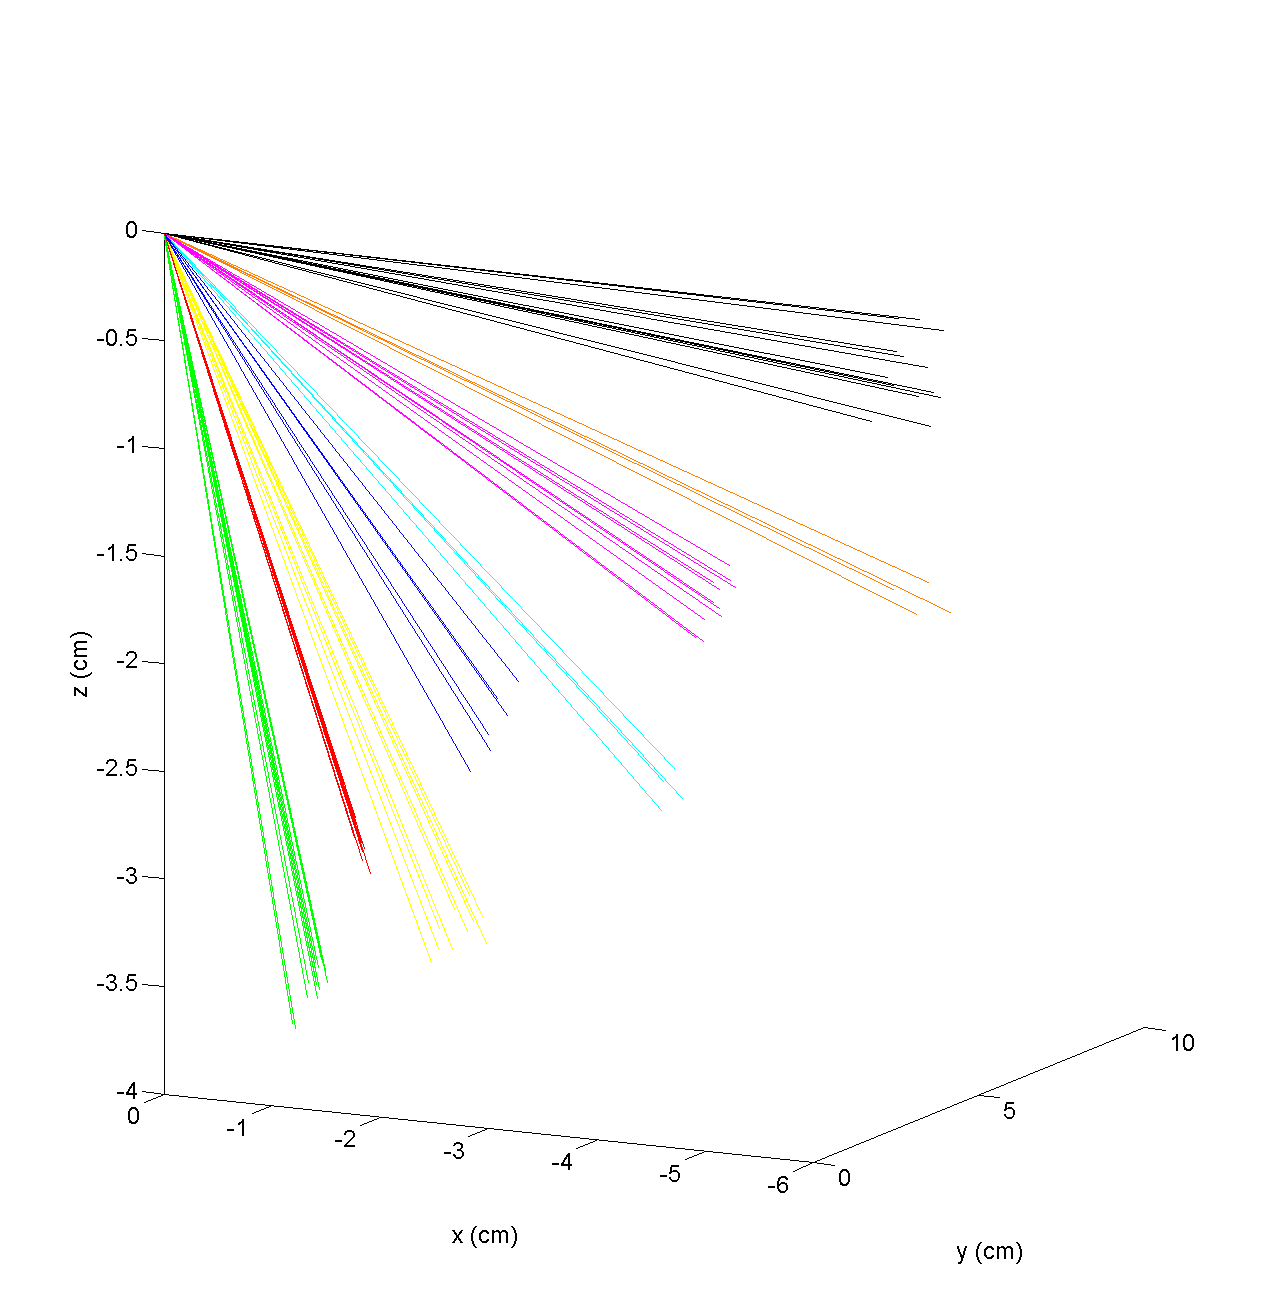
\includegraphics[height=8cm]{points2errplot.png}
\caption{Vektorji napak pri pozicioniranju z uporabo dveh kamer.}
\label{vec2}
\end{figure}
\begin{figure}
\centering
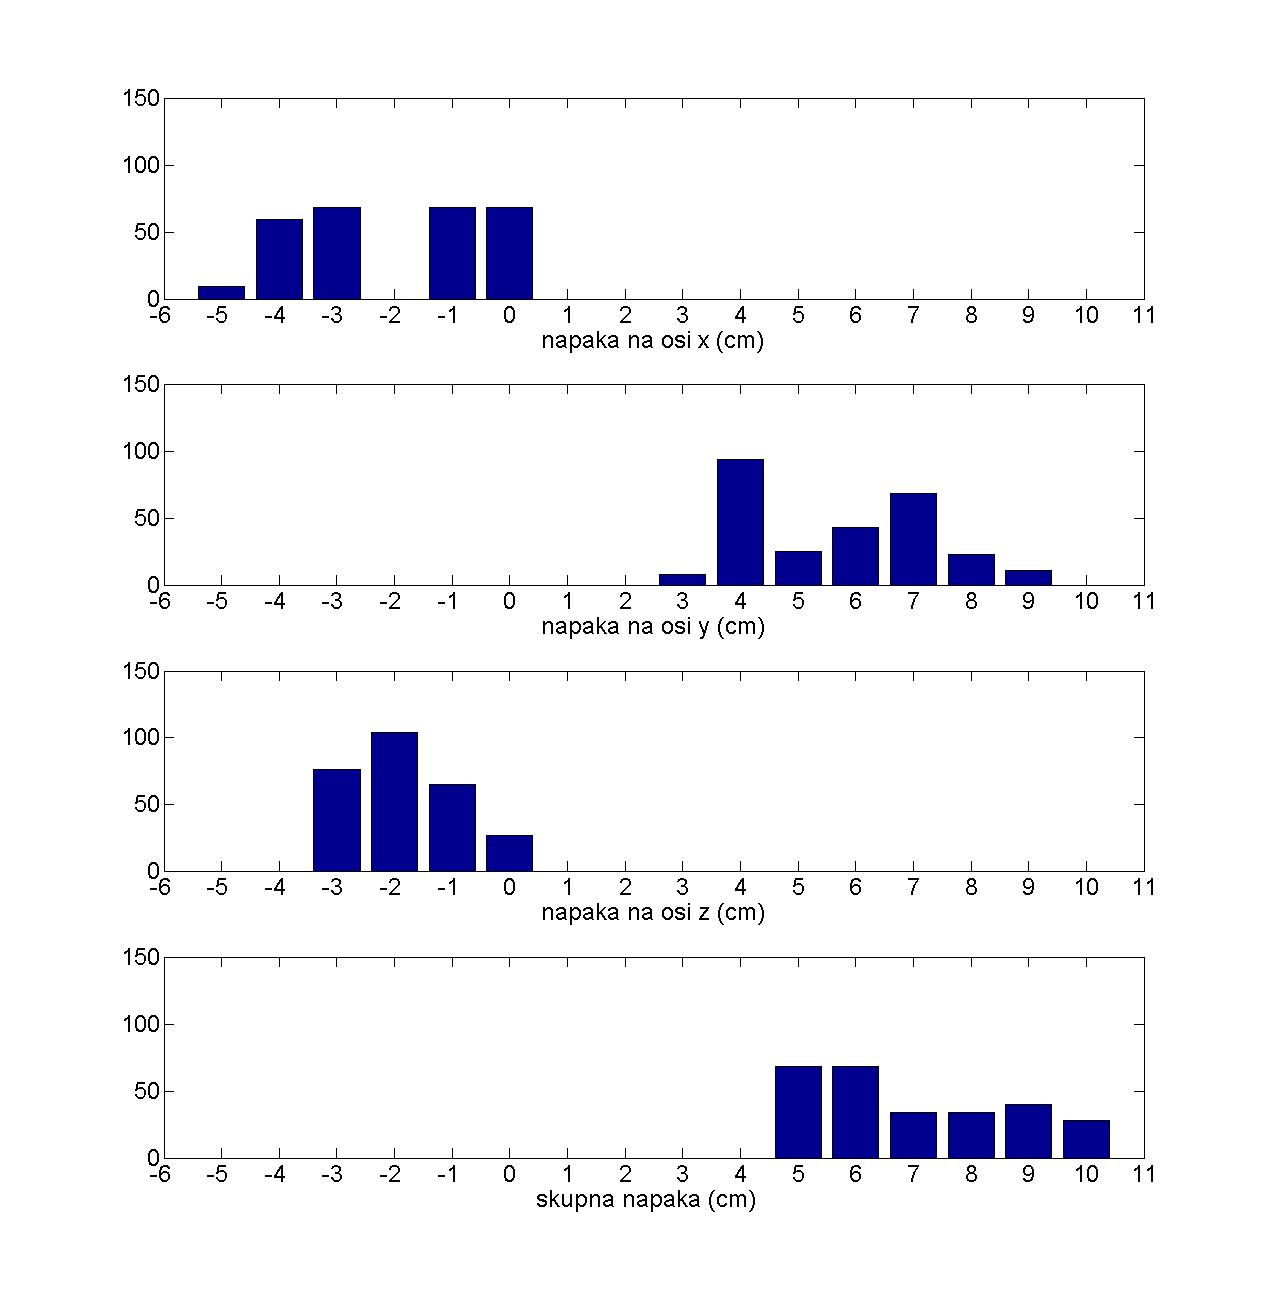
\includegraphics[height=10cm]{points2barplot.png}
\caption{Histogrami napak pri pozicioniranju z uporabo dveh kamer.}
\label{bar2}
\end{figure}

\begin{figure}
\centering
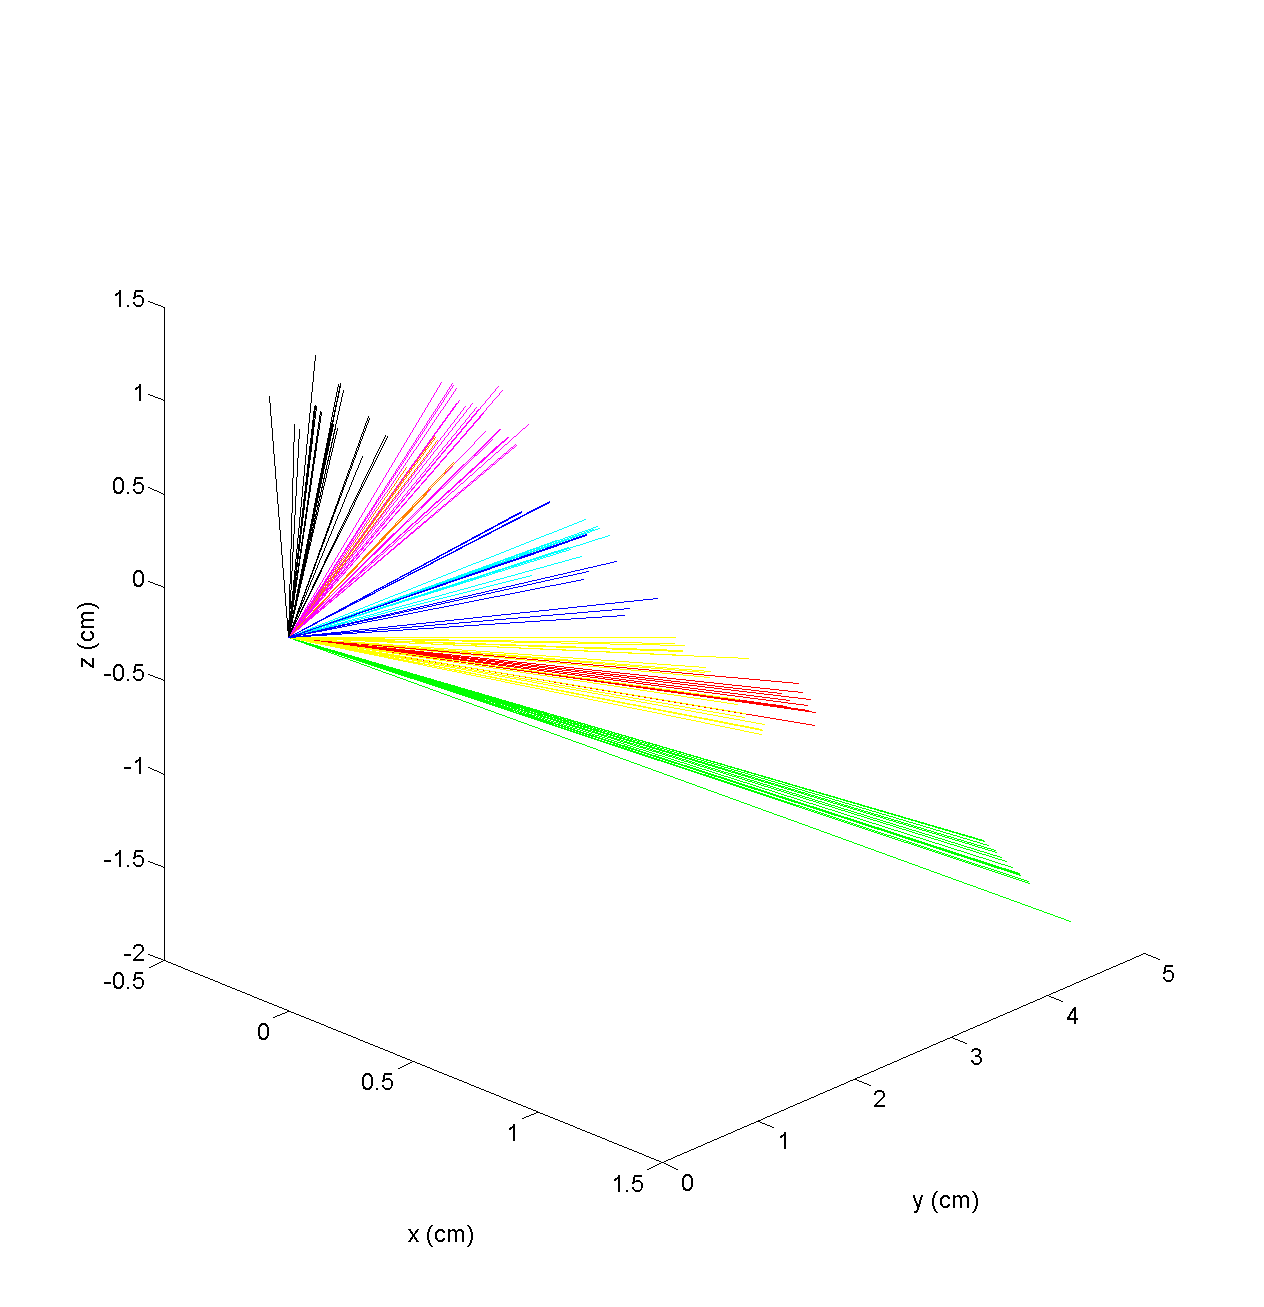
\includegraphics[height=8cm]{points3errplot.png}
\caption{Vektorji napak pri pozicioniranju z uporabo treh kamer.}
\label{vec3}
\end{figure}
\begin{figure}
\centering
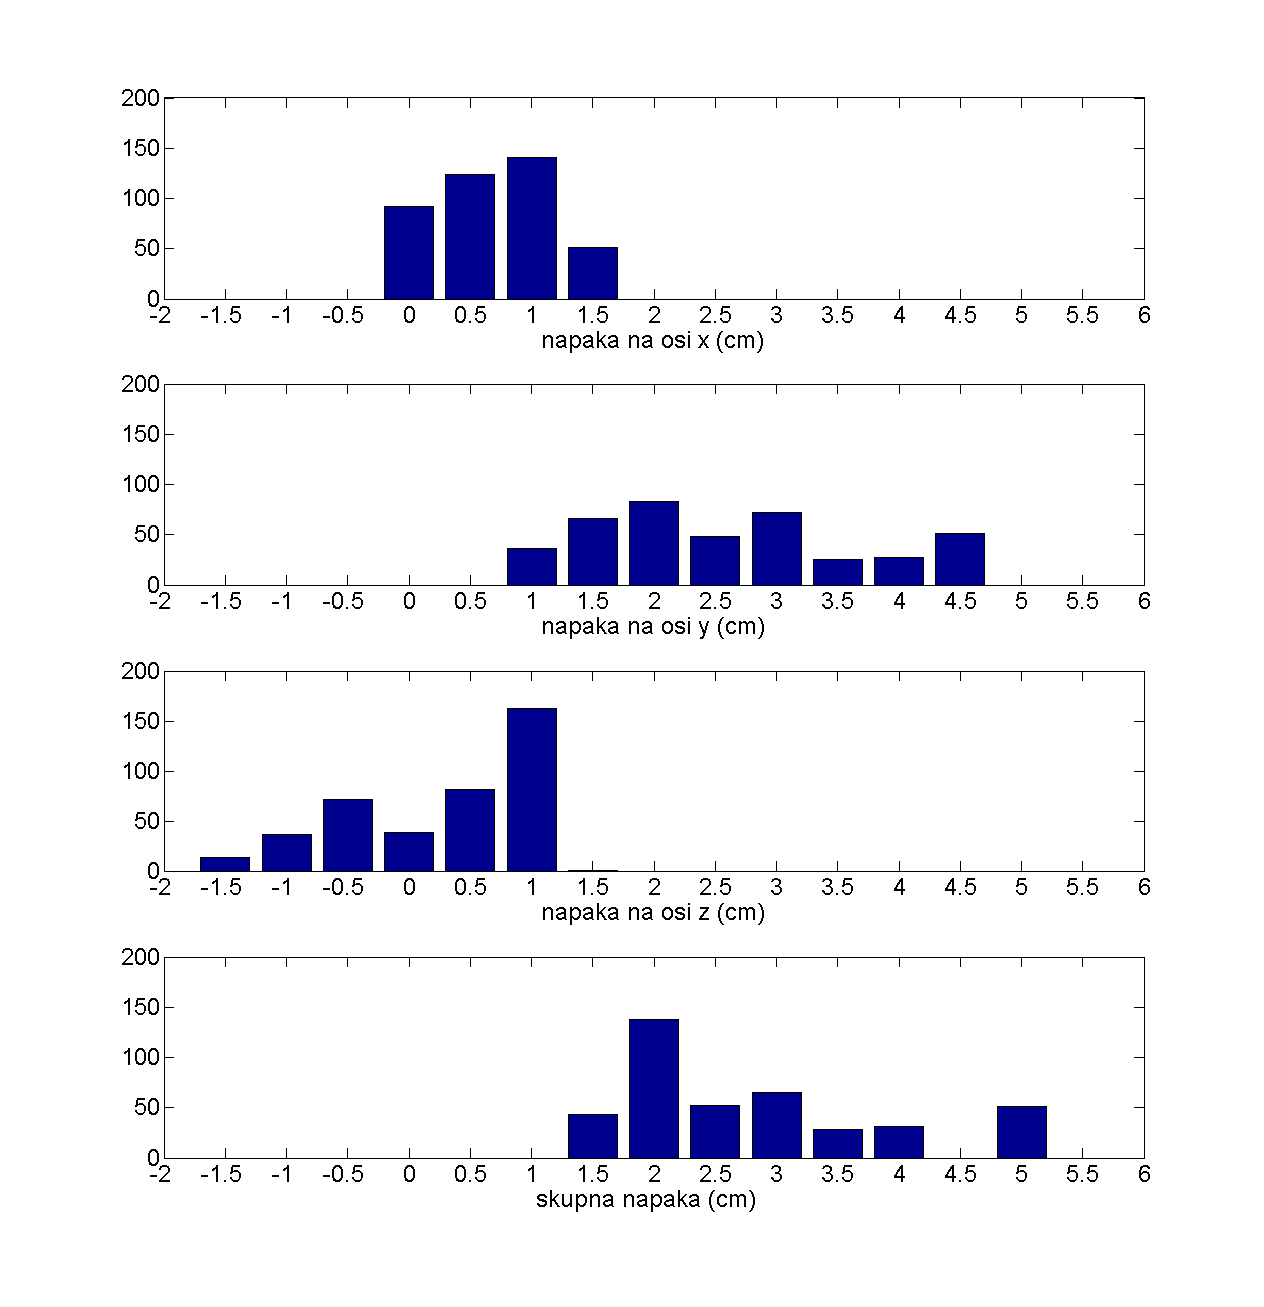
\includegraphics[height=10cm]{points3barplot.png}
\caption{Histogrami napak pri pozicioniranju z uporabo treh kamer.}
\label{bar3}
\end{figure}

\begin{figure}
\centering
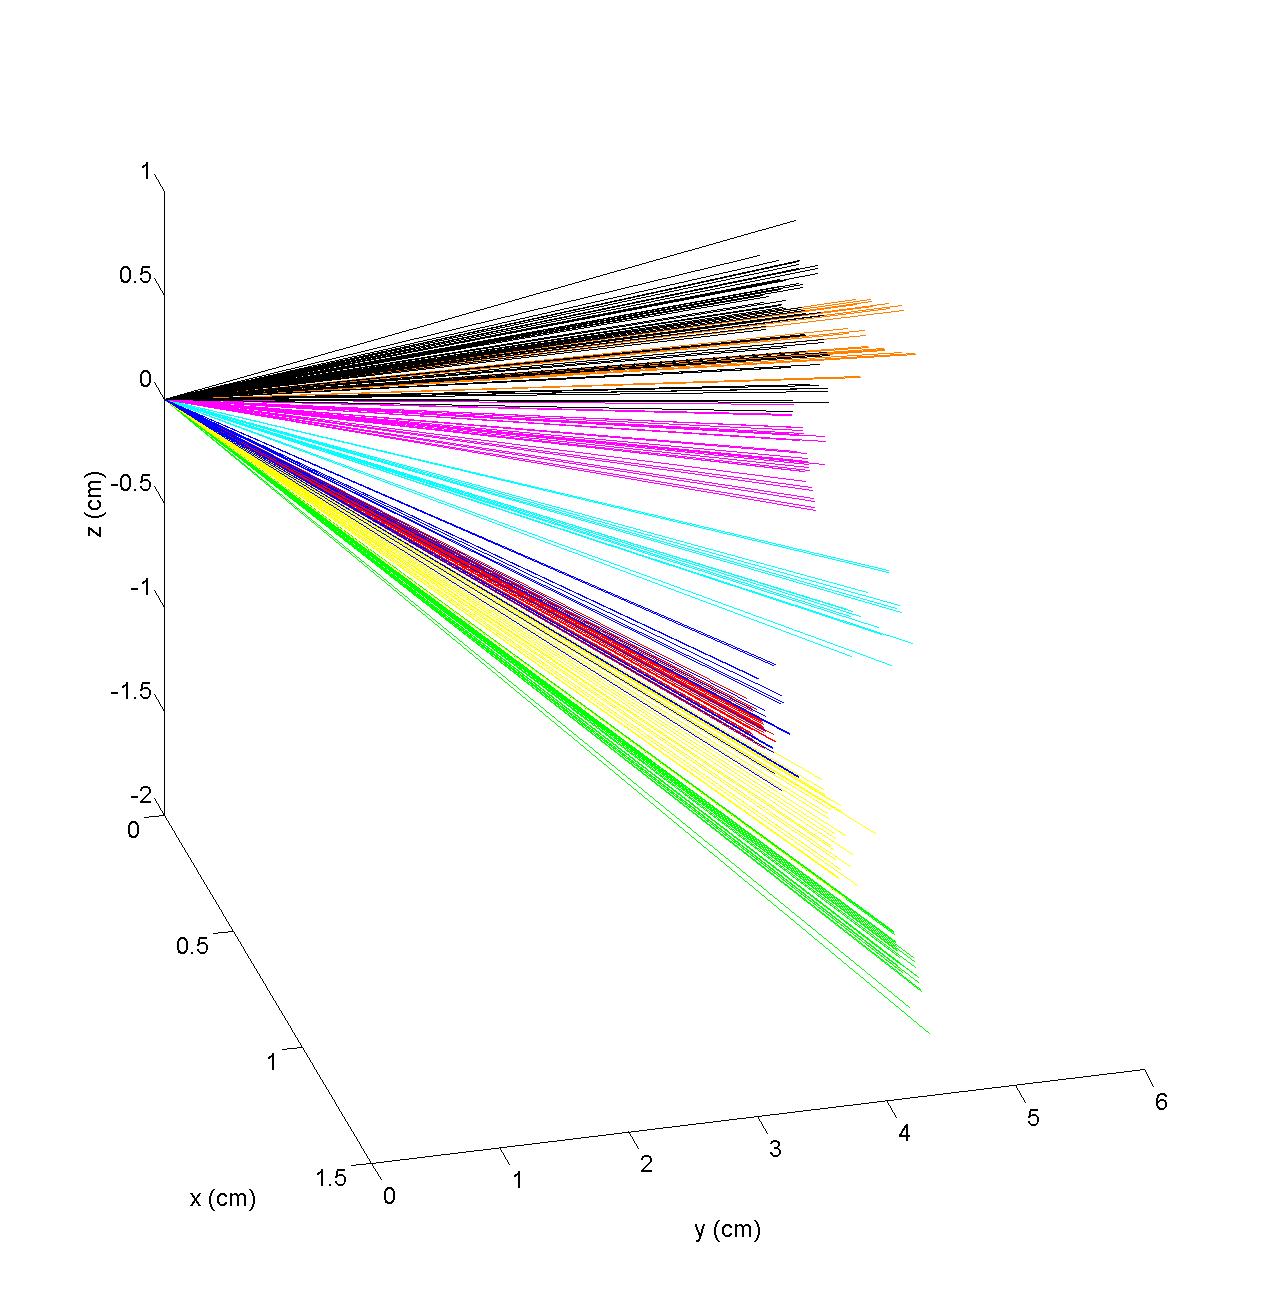
\includegraphics[height=8cm]{points4errplot.png}
\caption{Vektorji napak pri pozicioniranju z uporabo štirih kamer.}
\label{vec4}
\end{figure}
\begin{figure}
\centering
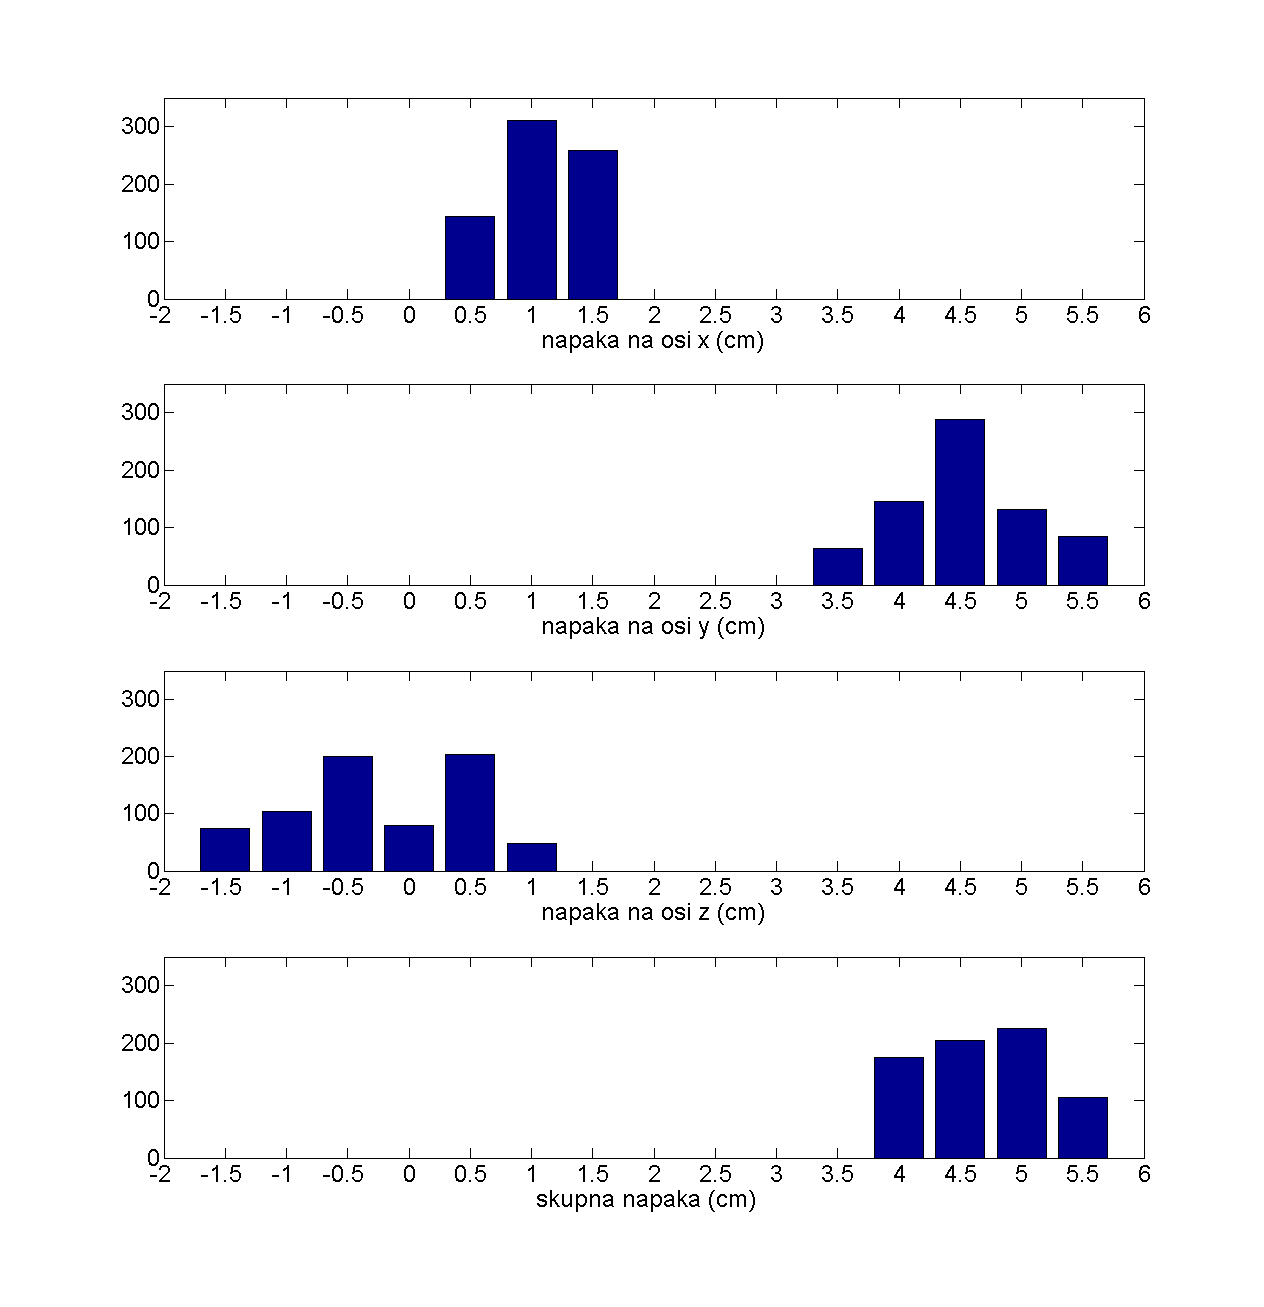
\includegraphics[height=10cm]{points4barplot.png}
\caption{Histogrami napak pri pozicioniranju z uporabo štirih kamer.}
\label{bar4}
\end{figure}


Na slikah \ref{vec2}, \ref{vec3} in \ref{vec4} so vizualizirani vektorji napak za meritve iz tabele \ref{positionerrortable}. Barve vektorjev predstavljajo različne točke iz tabele \ref{measuringptstab}. Hitro lahko opazimo, da napake niso naključne ampak strukturirane. Na slikah \ref{bar2}, \ref{bar3} in \ref{bar4} pa so prikazani histogrami napak. Pri vseh meritvah je največja napaka na osi $y$. Kalibracijske točke za zunanje parametre kamer (tabela \ref{pointpairs}) imajo veliko večjo varianco v smeri $x$, zato morda $y$ komponenta ni dovolj natančno določena.

\section{Natančnost trajektorije}
Trajektorijo dobimo tako, da združimo meritve skozi čas. Slike prikazujejo zaznane trajektorije, ki so za zaznavanje lokacij uporabile različne kombinacije kamer. Z rdečo barvo je označena točna trajektorija, z zeleno pa zaznana trajektorija. Trajektorija je lomljenka, ki jo določajo točke v tabeli \ref{trajectory}.

\begin{table}[H]
\centering
\begin{tabular}{| c | c | c |}
\hline
x ($cm$) & y ($cm$) & z ($cm$) \\
\hline
0 & 40 & 76 \\
0 & 80 & 76 \\
40 & 80 & 76 \\
40 & 40 & 76 \\
80 & 40 & 76 \\
80 & 80 & 76 \\
120 & 80 & 76 \\
120 & 40 & 76 \\
\hline
\end{tabular}
\caption{Referenčne točke za meritve v prostoru.}
\label{trajectory}
\end{table}

\begin{figure}
\centering
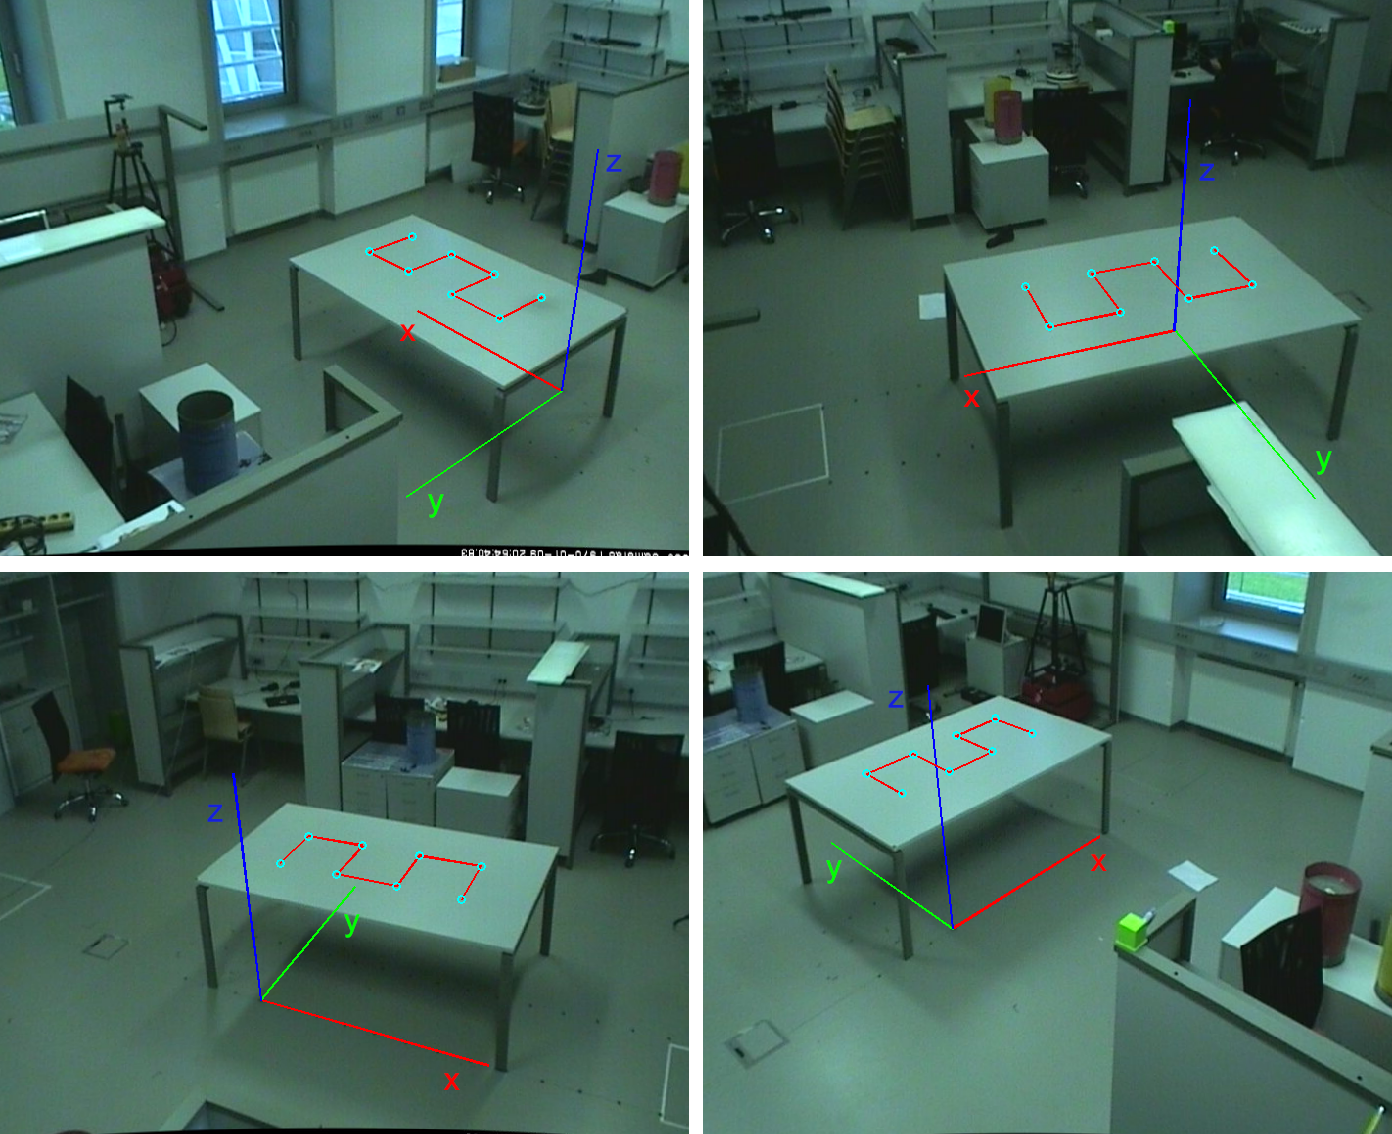
\includegraphics[width=\textwidth,height=\textheight,keepaspectratio]{path_layout.png}
\caption{Trajektorija je lomljenka označena z rdečimi daljicami.}
\label{accuracy_points}
\end{figure}

\begin{figure}
\centering
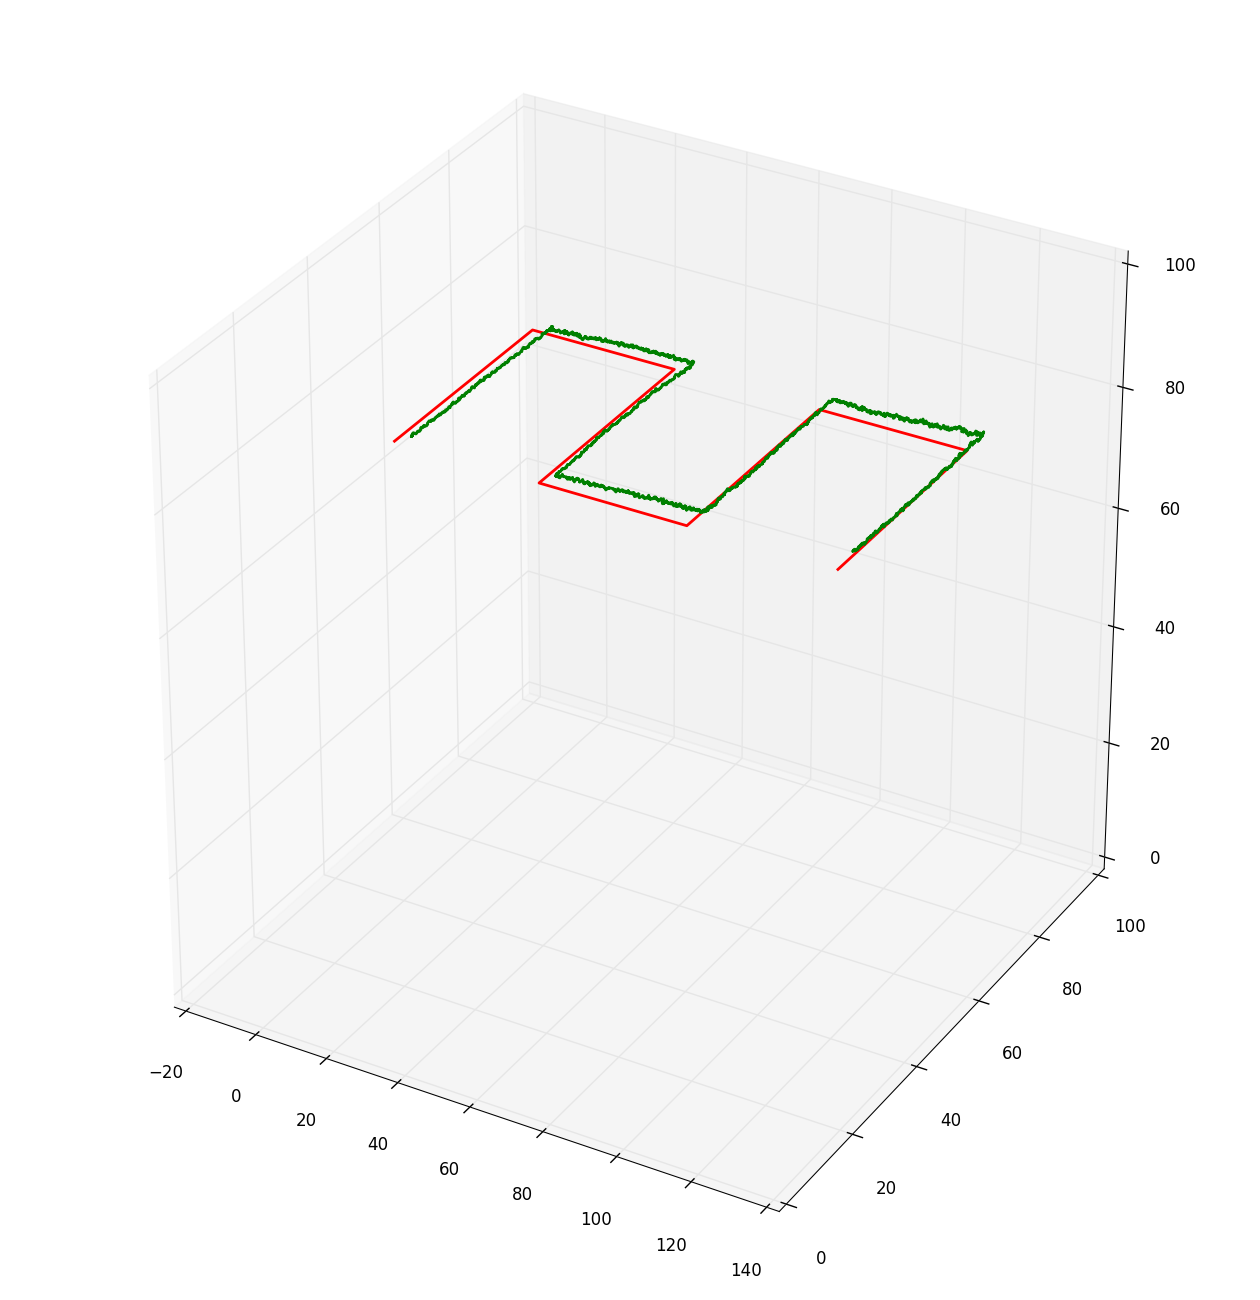
\includegraphics[width=10cm]{1234.png}
\caption{Triangulacija z vsemi kamerami.}
\end{figure}

\begin{figure}
    \centering
    \begin{subfigure}[t]{0.5\textwidth}
        \centering
        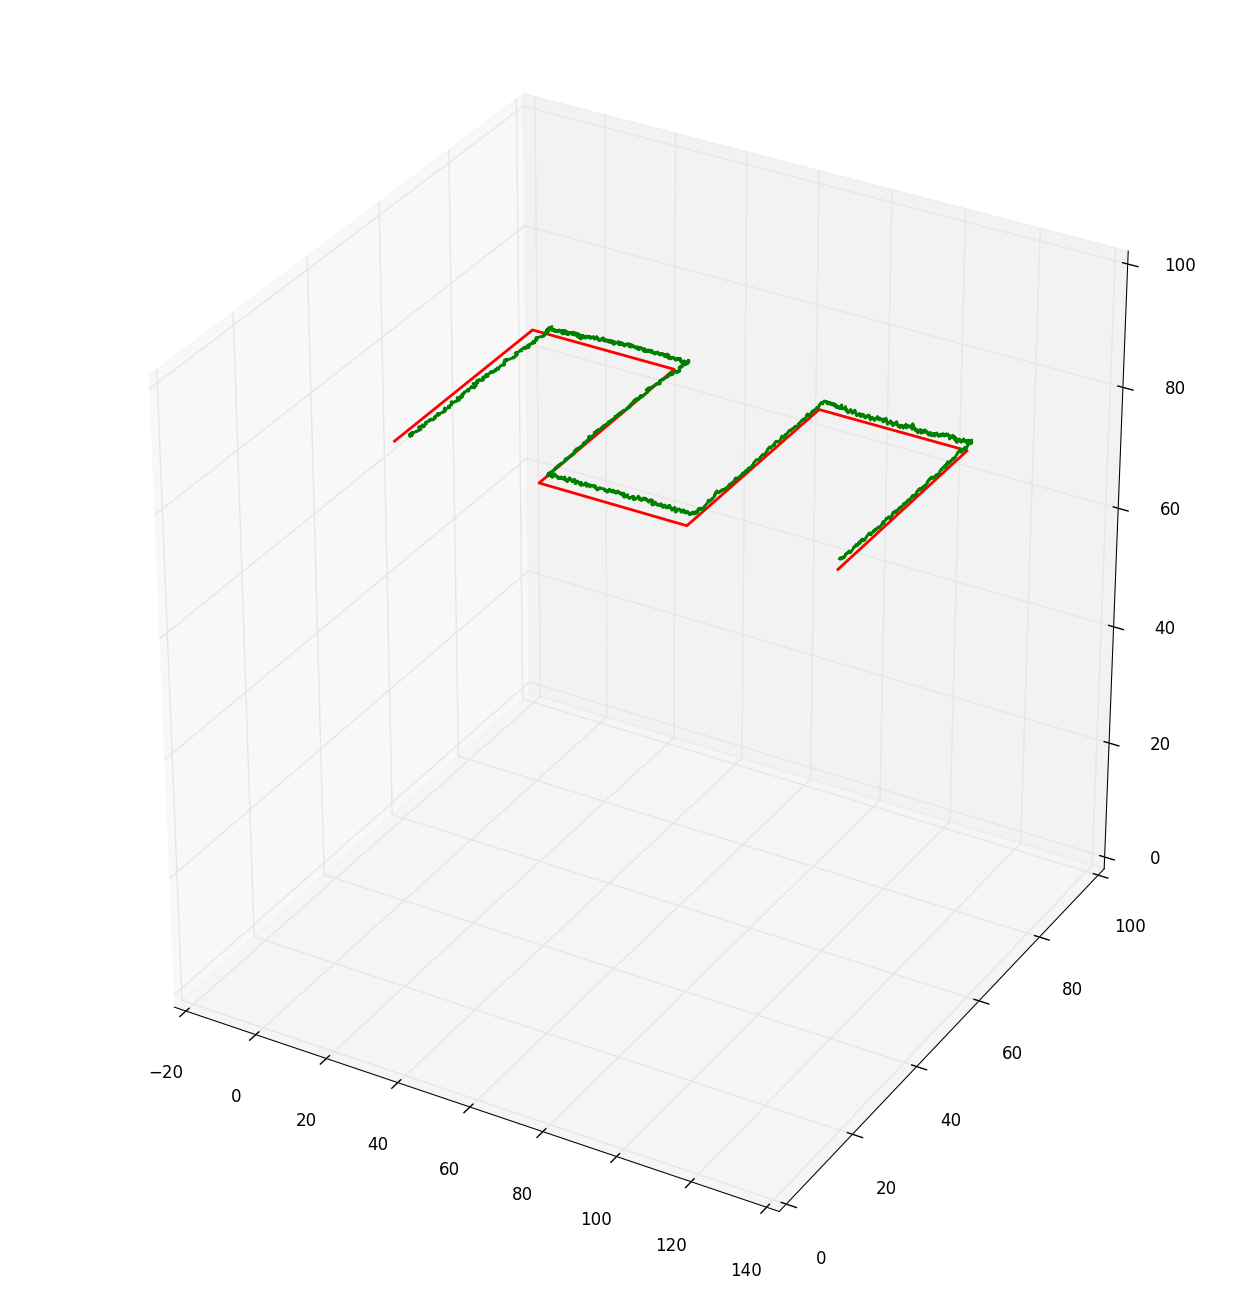
\includegraphics[width=6cm]{123.png}
        \caption{Kamera 1, 2 in 3.}
    \end{subfigure}~
    \begin{subfigure}[t]{0.5\textwidth}
        \centering
        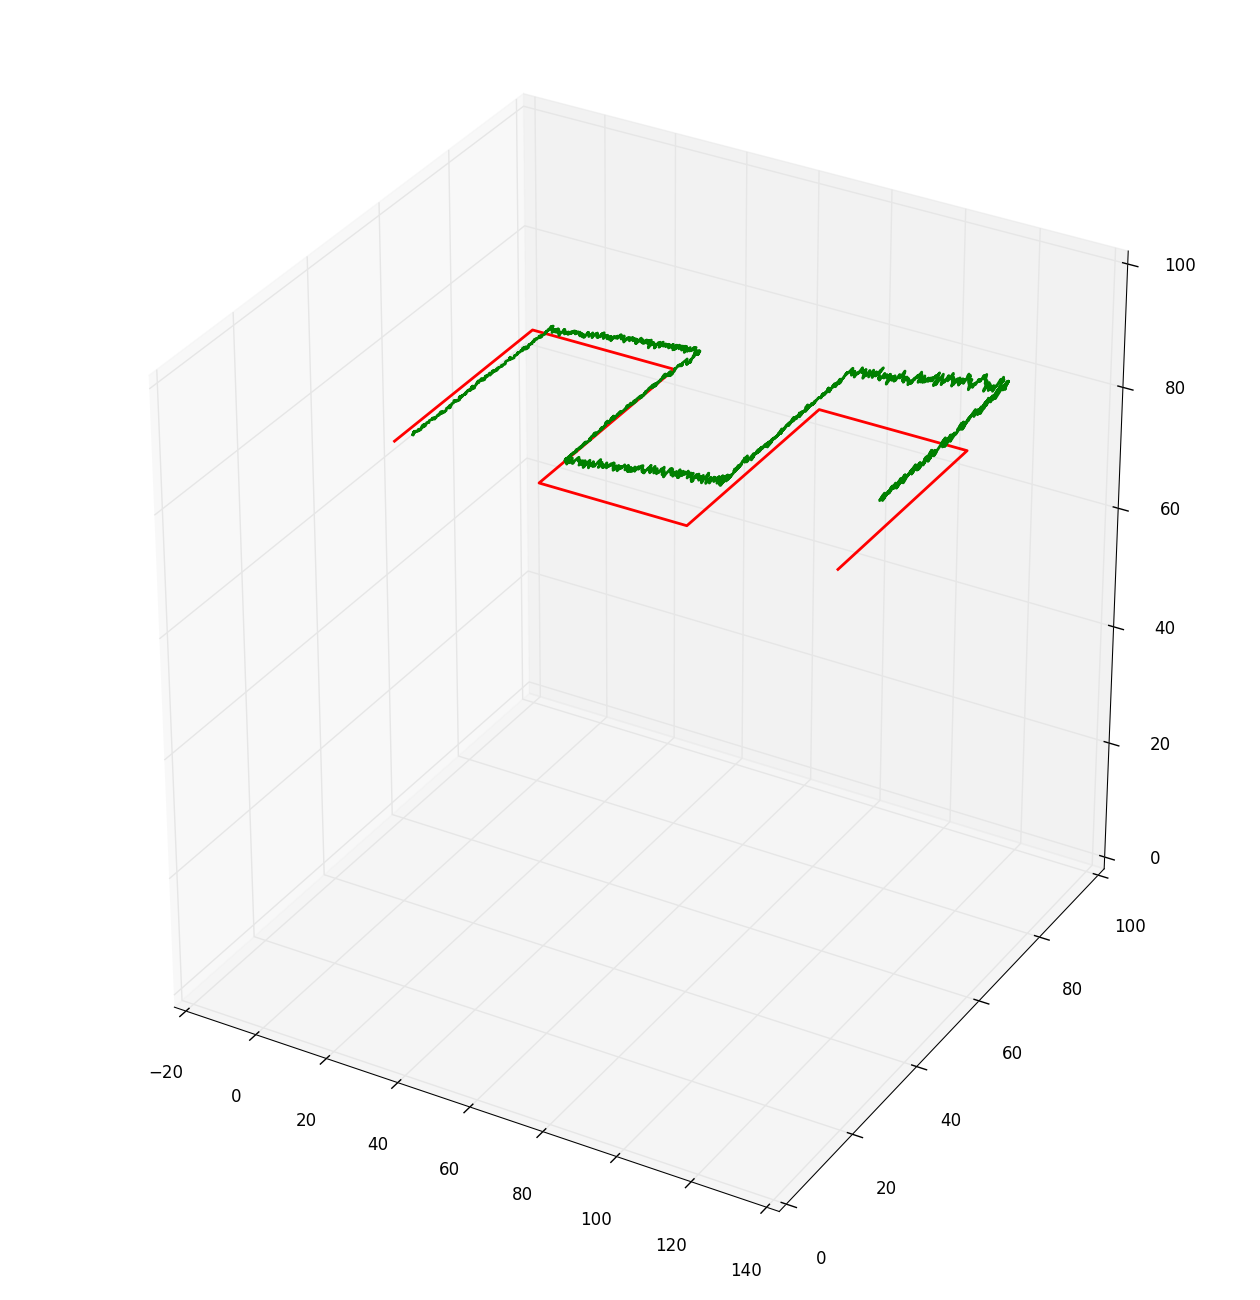
\includegraphics[width=6cm]{134.png}
        \caption{Kamera 1, 3 in 4.}
    \end{subfigure}
    
    \begin{subfigure}[t]{0.5\textwidth}
        \centering
        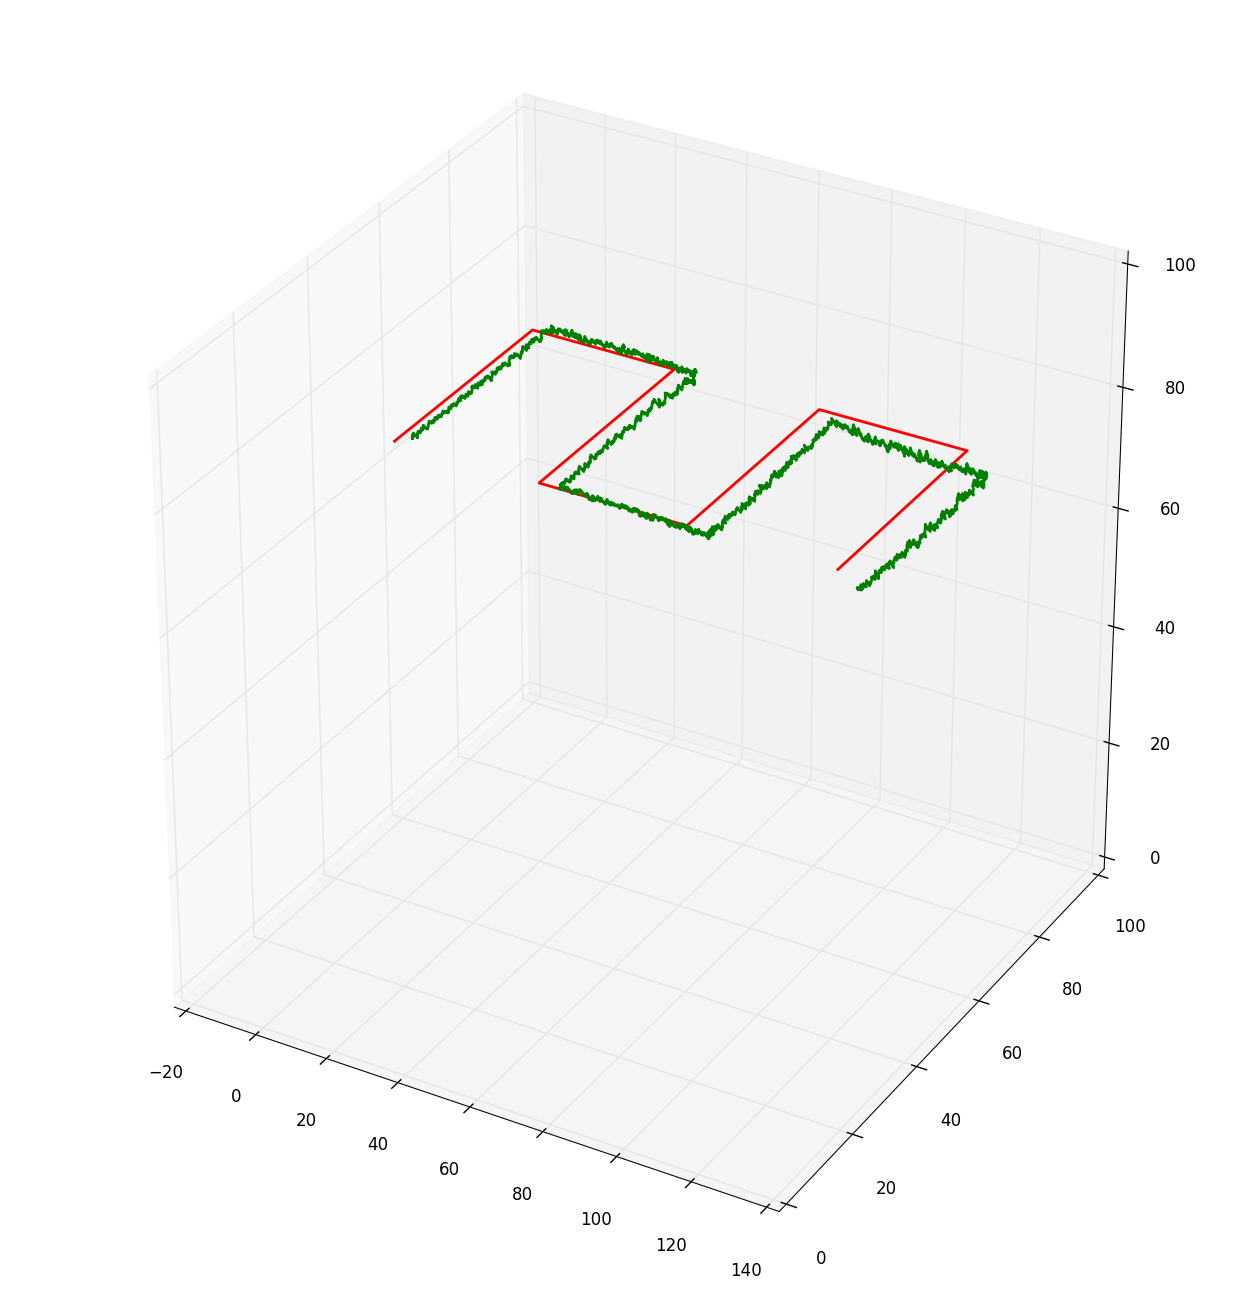
\includegraphics[width=6cm]{124.png}
        \caption{Kamera 1, 2 in 4.}
    \end{subfigure}~
    \begin{subfigure}[t]{0.5\textwidth}
        \centering
        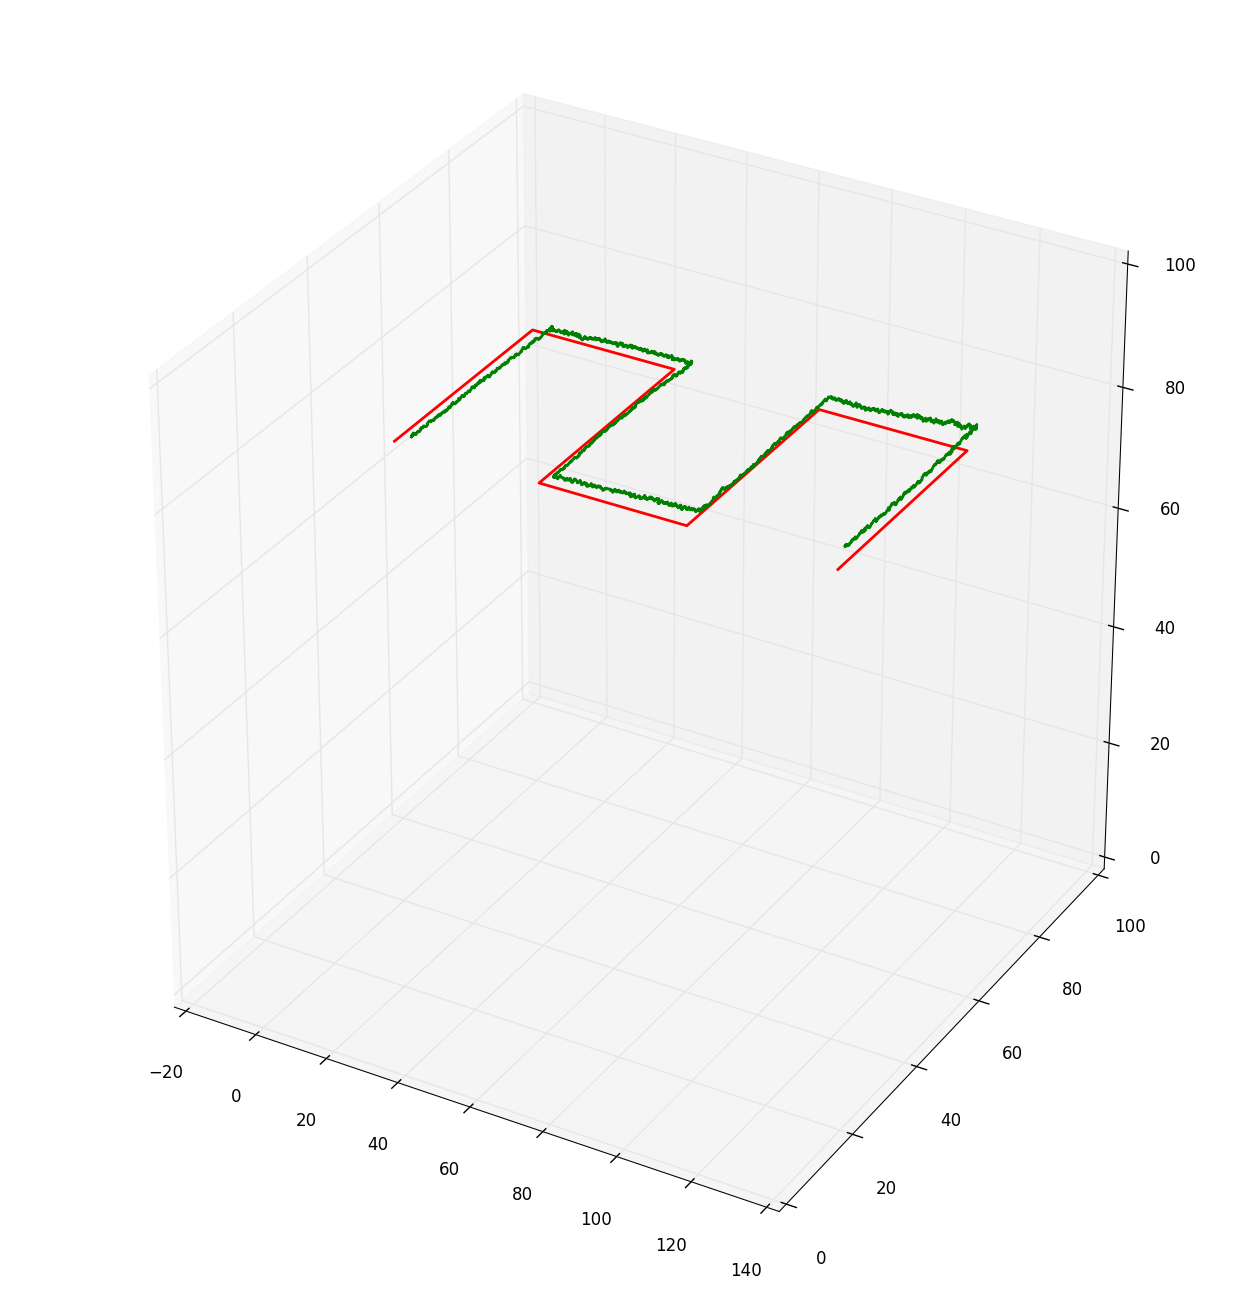
\includegraphics[width=6cm]{234.png}
        \caption{Kamera 2, 3 in 4.}
    \end{subfigure}
    \caption{Triangulacija z vsemi trojčki kamer.}
\end{figure}

\begin{figure}
    \centering
    \begin{subfigure}[t]{0.5\textwidth}
        \centering
        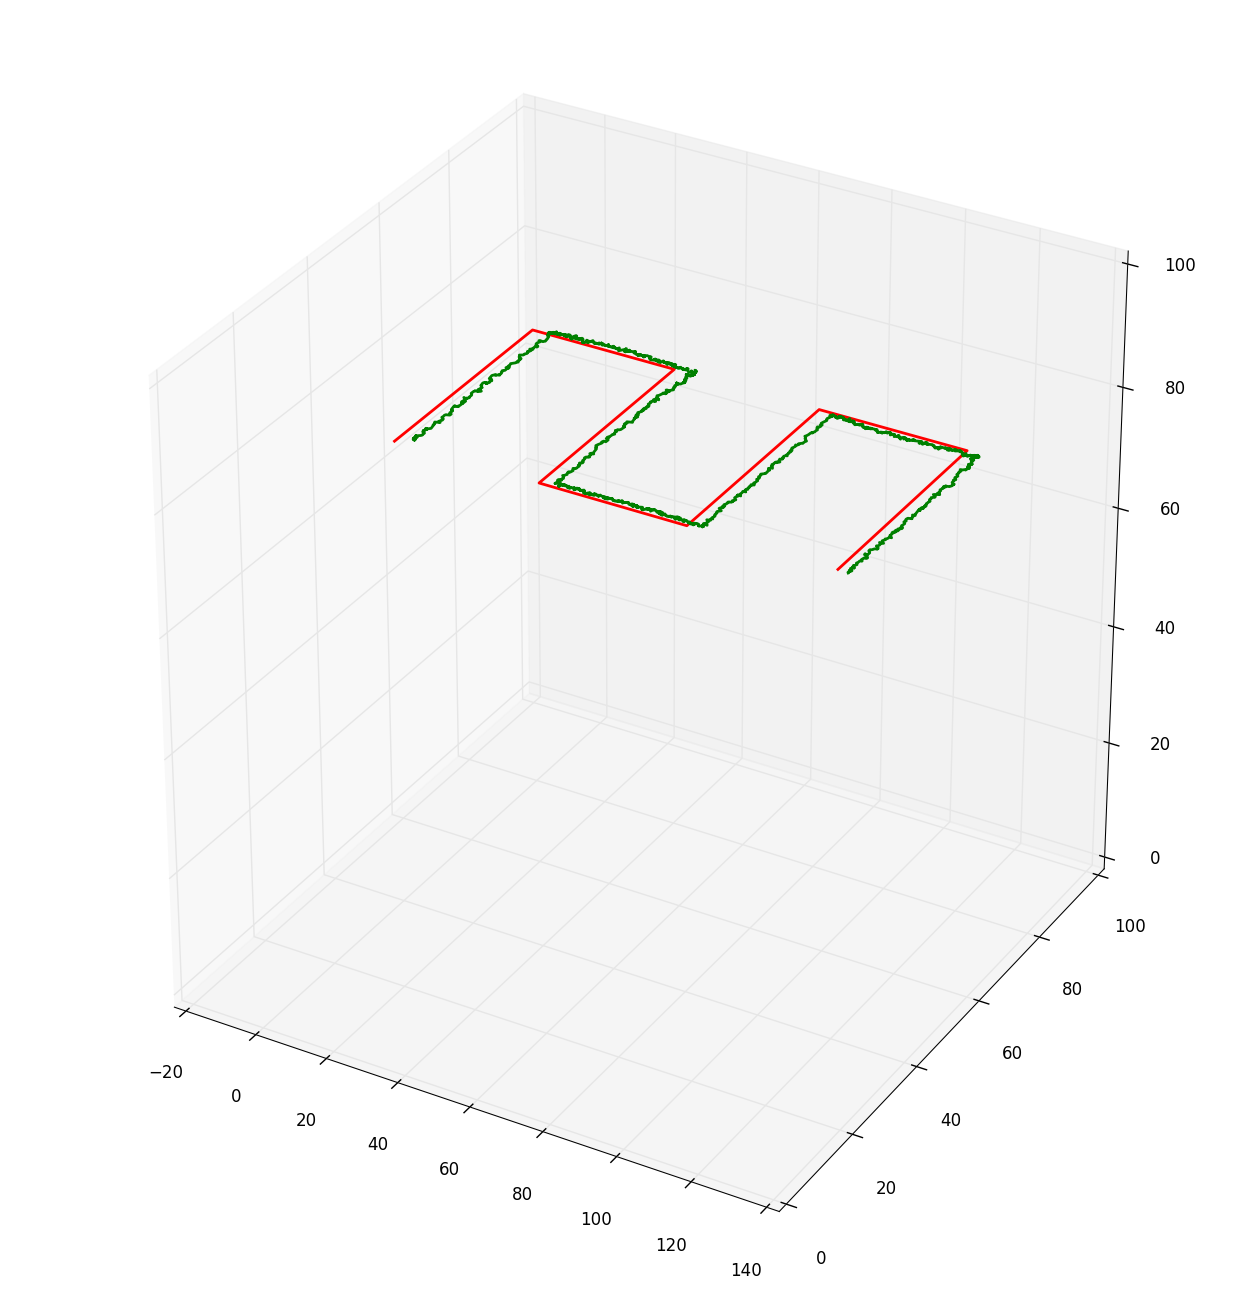
\includegraphics[width=6cm]{12.png}
        \caption{Kamera 1 in 2.}
    \end{subfigure}~
    \begin{subfigure}[t]{0.5\textwidth}
        \centering
        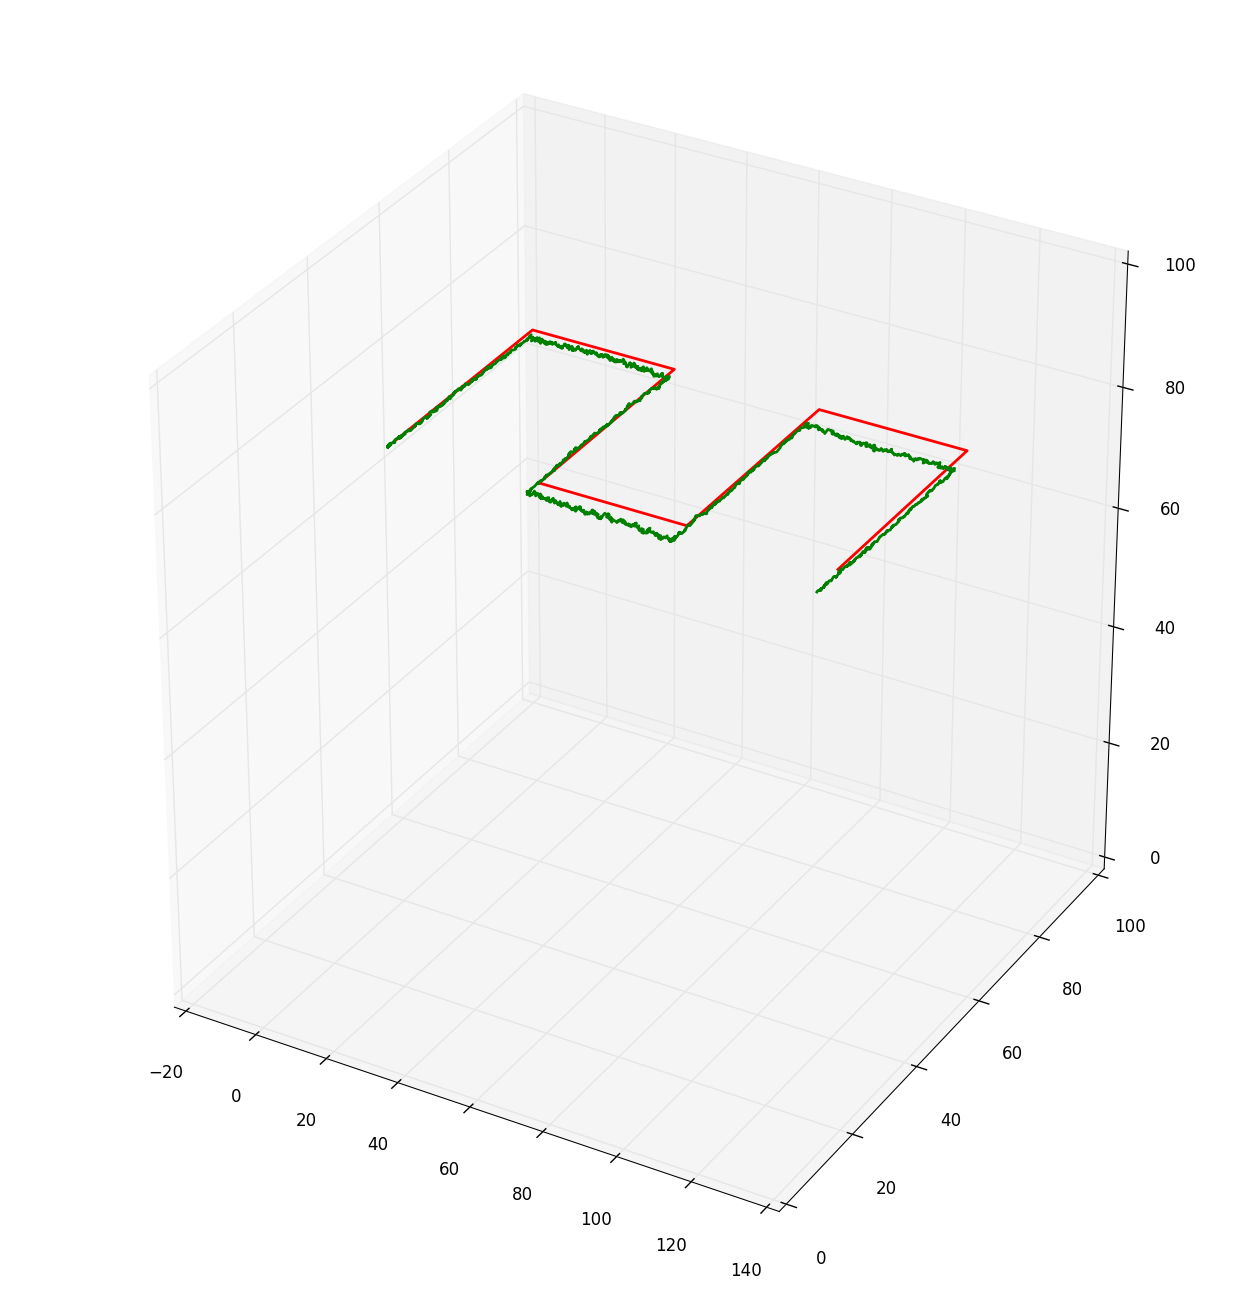
\includegraphics[width=6cm]{13.png}
        \caption{Kamera 1 in 3.}
    \end{subfigure}
    
    \begin{subfigure}[t]{0.5\textwidth}
        \centering
        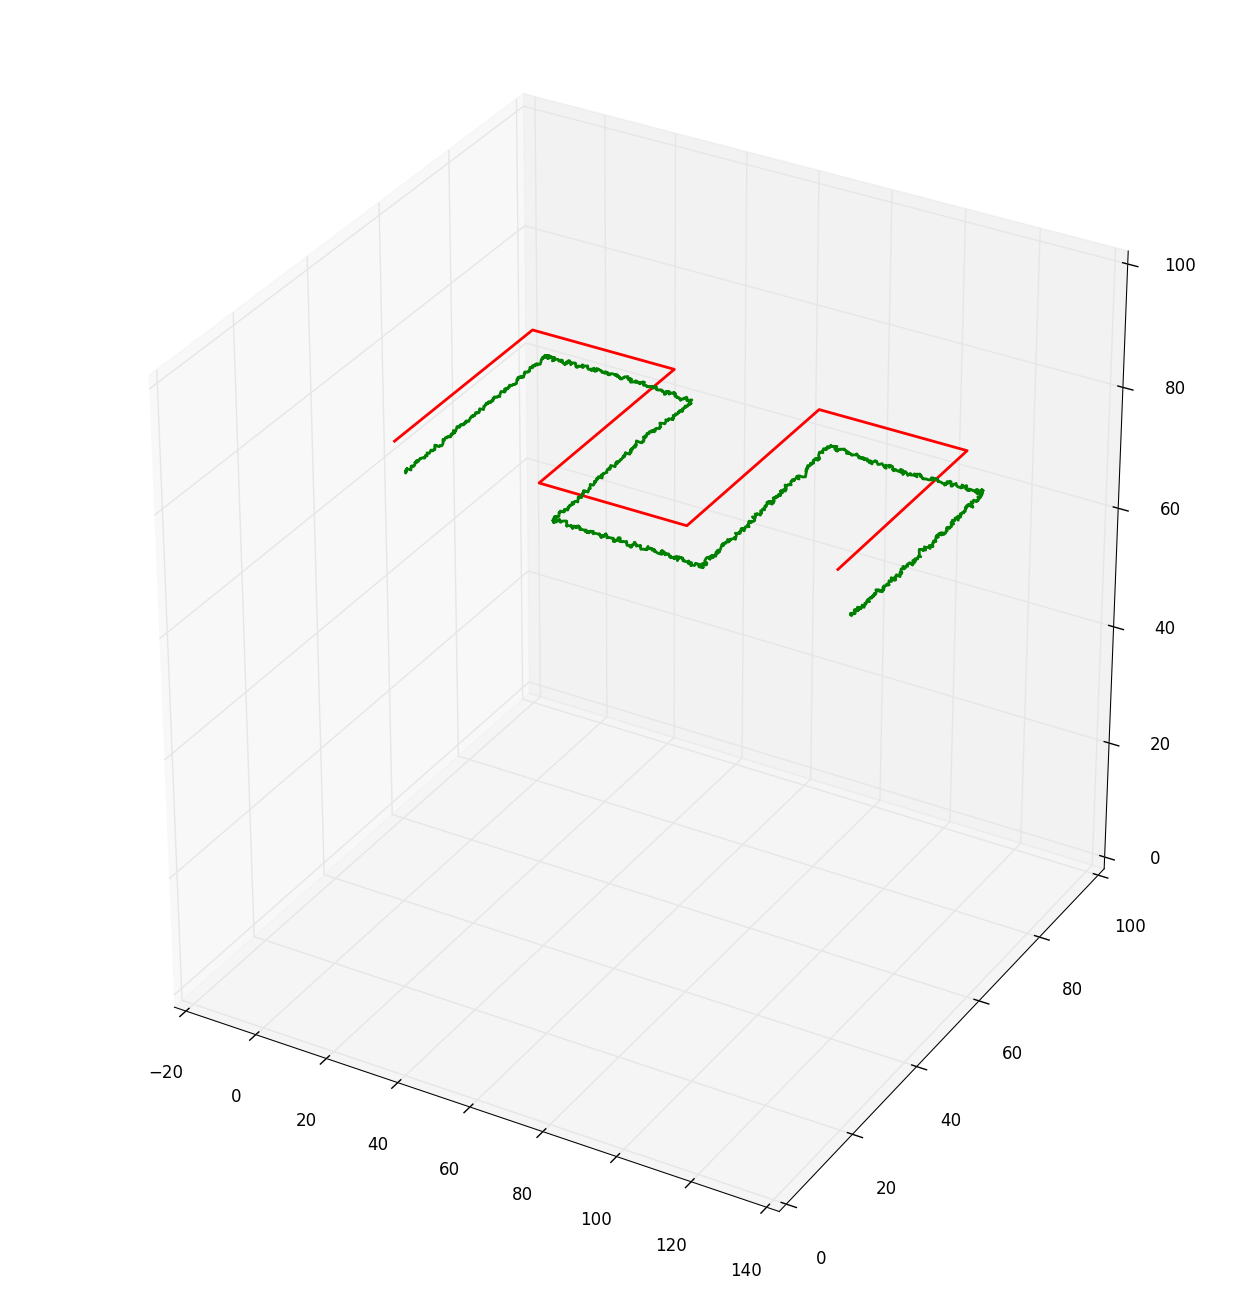
\includegraphics[width=6cm]{14.png}
        \caption{Kamera 1 in 4.}
    \end{subfigure}~
    \begin{subfigure}[t]{0.5\textwidth}
        \centering
        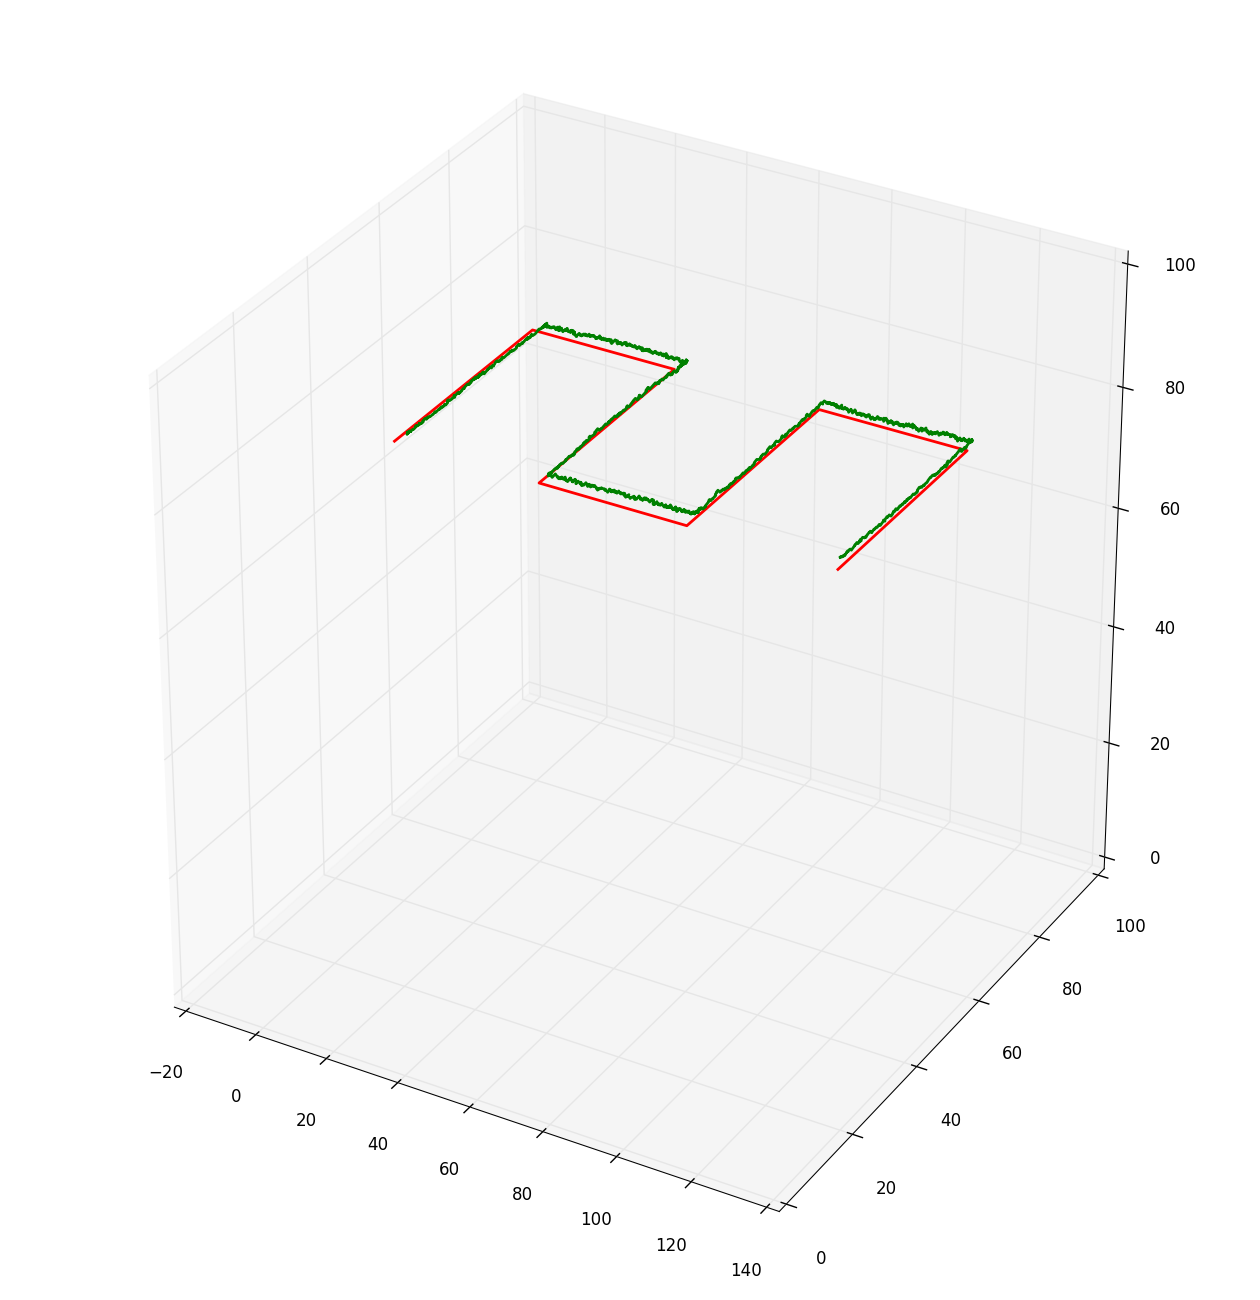
\includegraphics[width=6cm]{23.png}
        \caption{Kamera 2 in 3.}
    \end{subfigure}
    
    \begin{subfigure}[t]{0.5\textwidth}
        \centering
        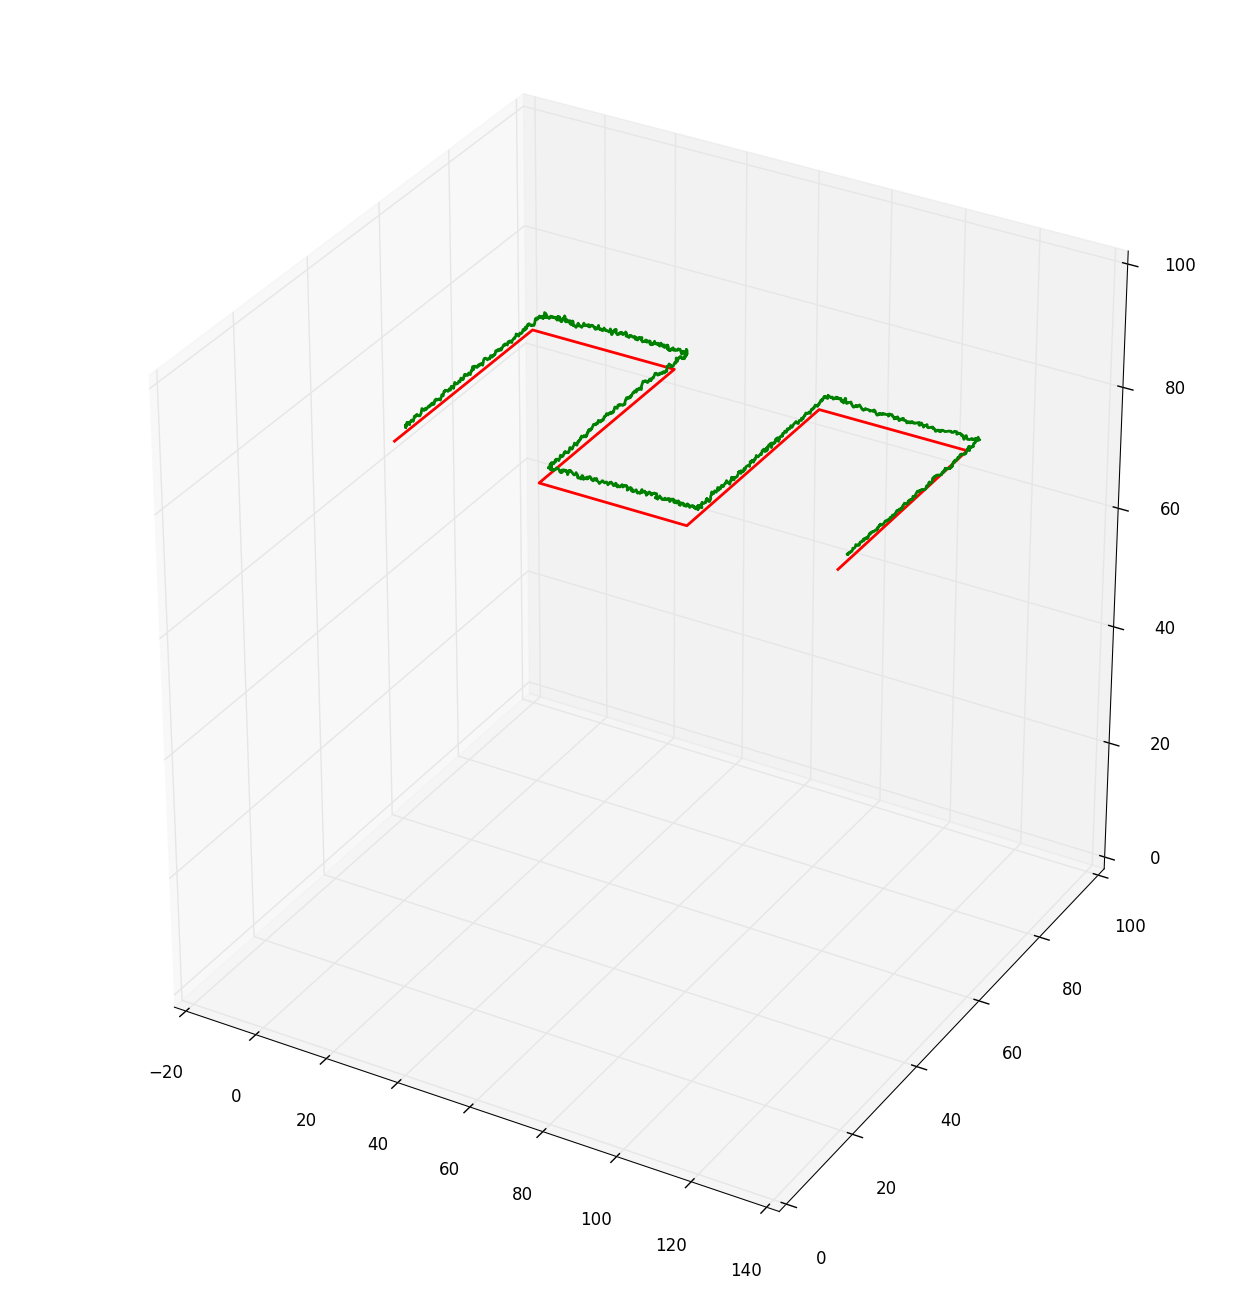
\includegraphics[width=6cm]{24.png}
        \caption{Kamera 2 in 4.}
    \end{subfigure}~
    \begin{subfigure}[t]{0.5\textwidth}
        \centering
        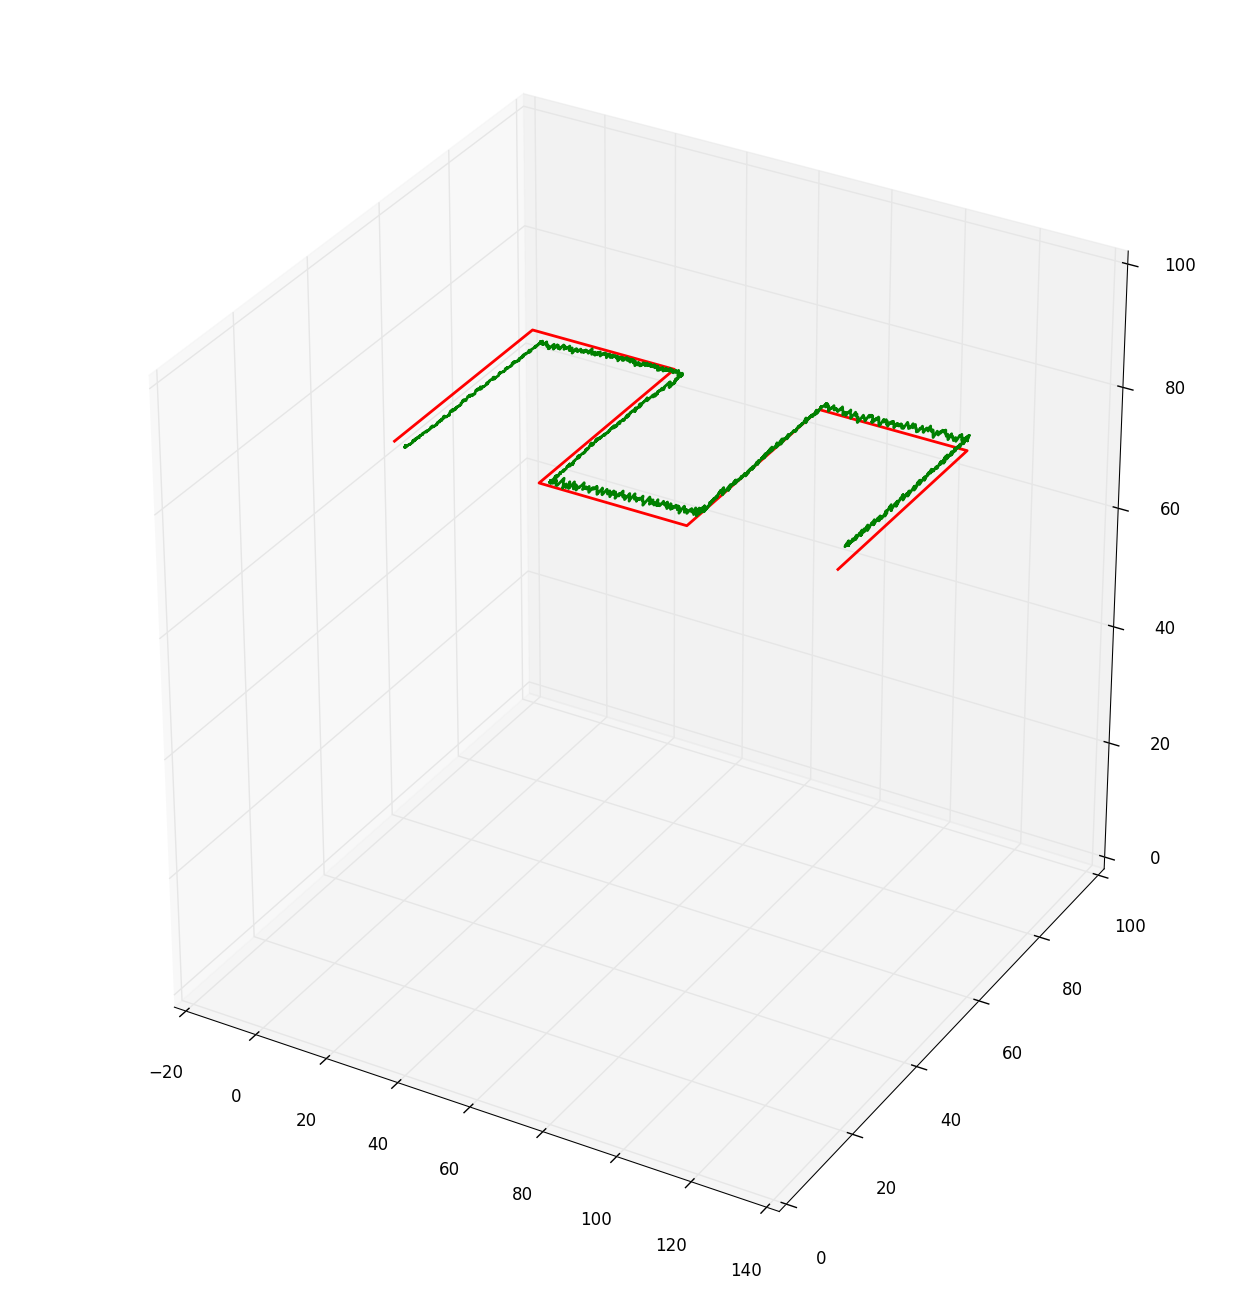
\includegraphics[width=6cm]{34.png}
        \caption{Kamera 3 in 4.}
    \end{subfigure}
    \caption{Triangulacija z vsemi pari kamer.}
\end{figure}

Iz slik se vidi, da je trajektorija, relativno na obliko, dobro določena, ampak narobe umeščena v prostor. Obstajata dva glavna razloga za napake v lokalizaciji: slaba kalibracija kamer ali slabo zaznavanje označevalnika. Napaka pri zaznavanju označevalnika je največ $1,5$ slikovnih pik, kar je premalo, da bi povzročilo tako drastične spremembe pri zaznavanju. Vsaka kamera je kalibrirana neodvisno od druge, zato je zelo verjetno, da je prostor za vsako kamero rahlo drugačen. To bi razložilo opazovano obnašanje zaznavanja. Triangulacija z večjim številom kamer v povprečju vrne boljši rezultat, saj se napake med seboj skoraj izničijo. Opazimo lahko, da triangulacija s prvo in četrto kamero povzroči največjo napako. 

\chapter{Zaključek}
V diplomski nalogi smo naredili večkamerni sistem za lokalizacijo objekta v prostoru. Uporabili smo štiri Axis 215 PTZ kamere in jih postavili v kote kvadratnega stropa sobe. Usmerjene so bile proti sredini tal. Z orodjem smo določili notranje parametre kamer, za izračun zunanjih parametrov pa smo uporabili metodi DLT in SVD. Zunanje parametre smo določili s koplanarnimi točkami v prostoru, kar v sistem enačb vnese dvoumnost rešitve (sučnost koordinatnega sistema). Pravilno rešitev izberemo ročno. 

Označevalnik zaznavamo s preprostim postopkom segmentacije, nato pa s slikovnimi momenti izračunamo njegovo masno središče. Sistem deluje v realnem času s 24 meritvami na sekundo. Rezultati so pokazali, da je natančnost zaznavanja označevalnika visoka (povprečno $0,85$ slikovnih pik napake).

Natančnost lokalizacije je v veliki meri odvisna od natančnosti kalibracije kamer in manj od zanavanja označevalnika. Prav tako je pomembno, katere kamere uporabimo pri triangulaciji. Sistem lahko uporabimo za opazovanje in merjenje trajektorije objekta.

Prostora za izboljšave je še veliko. Ker kamere nimajo sočasnega prožilca za zajem slik, lahko pride do majhne nesinhroniziranosti med slikami (trianguliramo s pozicijami označevalnika v različnih časih), kar pri velikih hitrostih objekta predstavlja velik problem. Sistem bi lahko izboljšali z interpolacijo lokacij označevalnika na slikah. Trenutno je potrebno za kalibracijo zunanjih paramterov ročno izbrati kalibracijske točke. Sistem bi lahko nadgradili tako, da kalibracija poteka avtomatizirano na podlagi vzorca v prostoru (npr. šahovnice). Nenazadnje pa je sistem zelo omejen z vrsto objekta, ki ga lokalizira (svetleč barvni označevalnik). Veliko bolj uporabno bi bilo implementirati splošni sledilnik, ki razlikuje med različnimi objekti na sliki in s tem omogoča sočasno lokalizacijo vseh objektov zanimanja.



\bibliography{bibliography}{}
\bibliographystyle{plain}
\end{document}

